\chapter{Perancangan}
\label{chap:perancangan}

\section{Rancangan Antarmuka}
    \begin{sidewaysfigure}
        \centering
        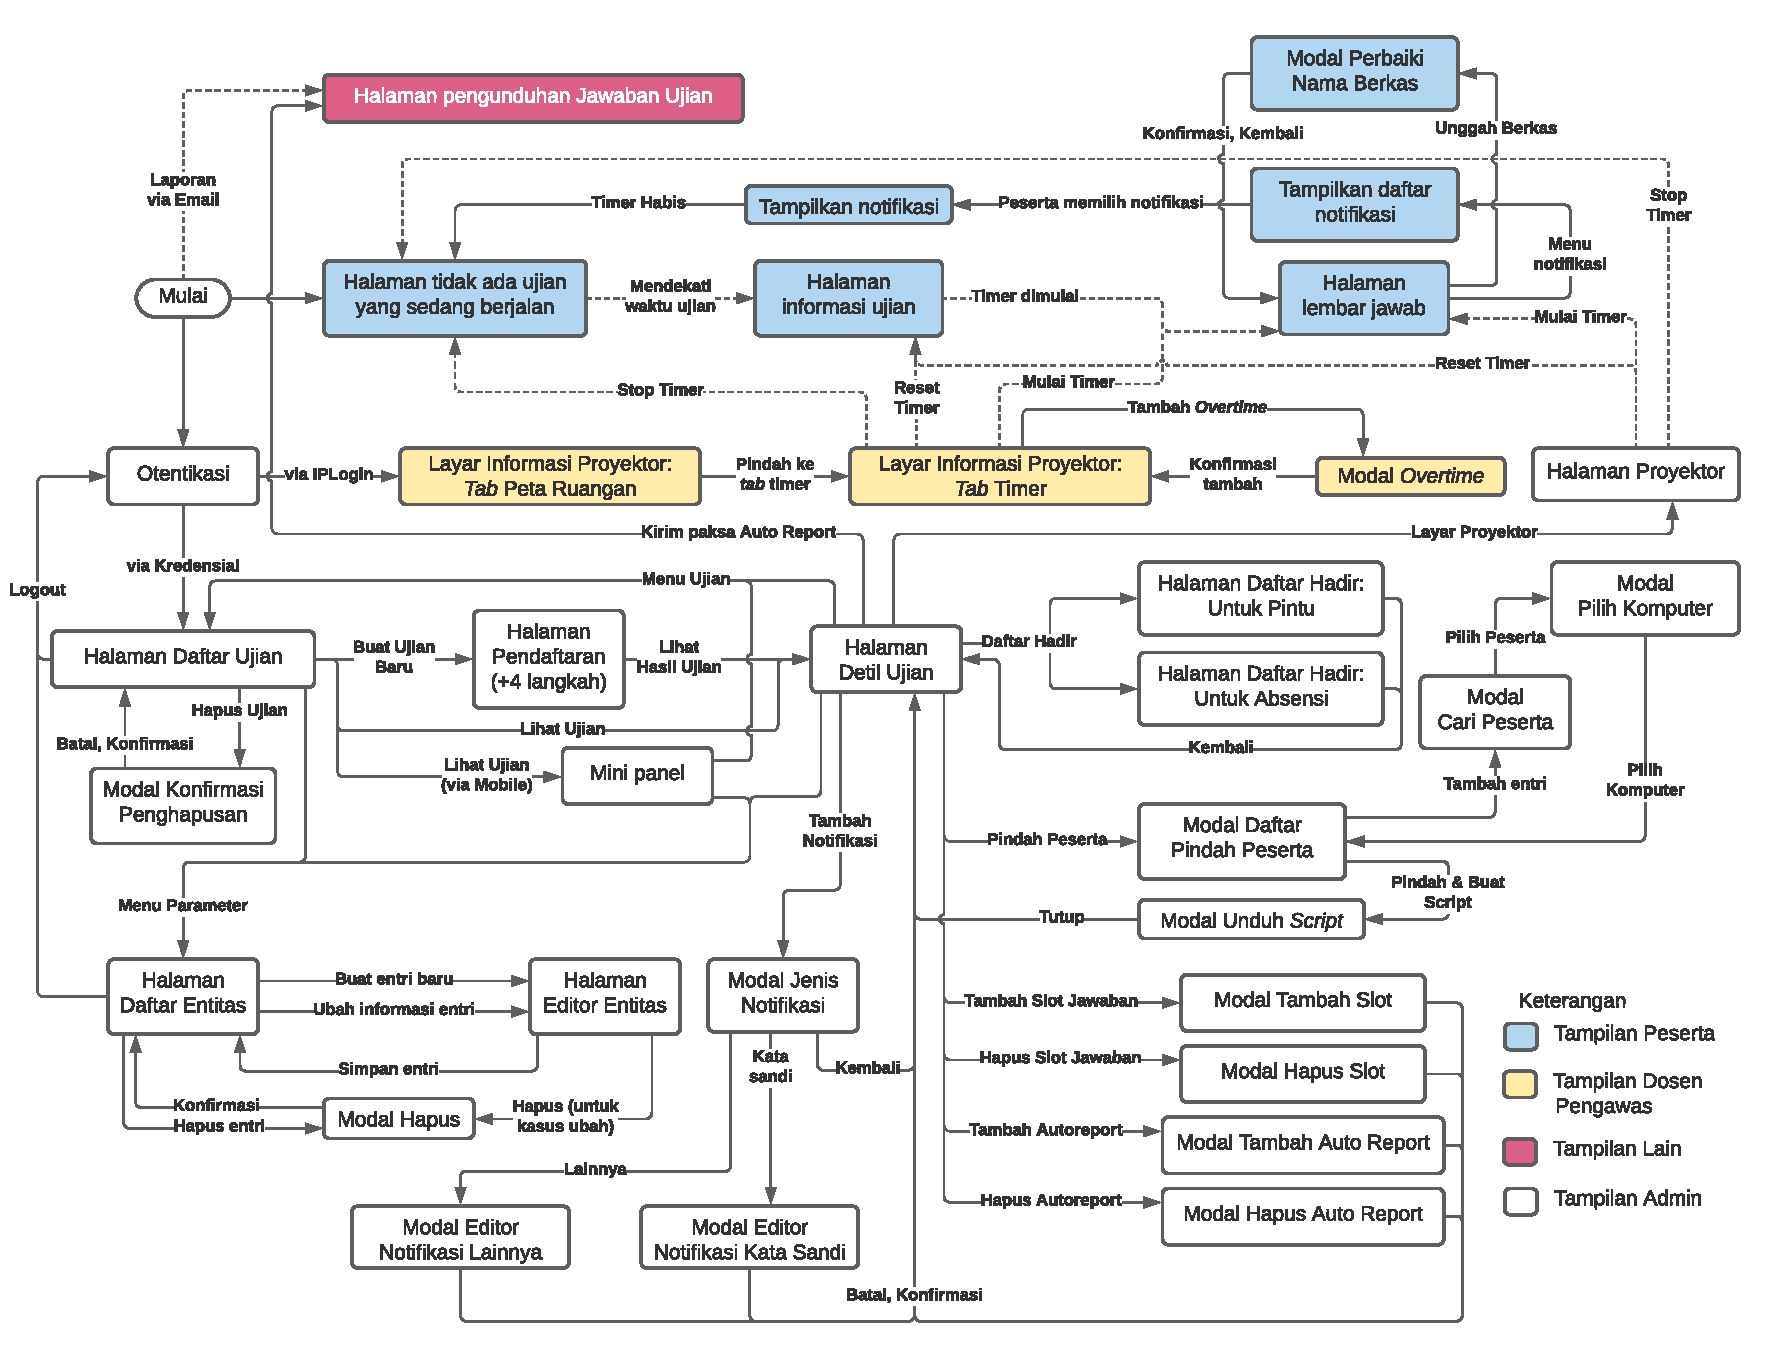
\includegraphics[height=0.7\paperwidth]{Gambar/Screenflow - Plumber.pdf}
        \caption{Diagram alur antarmuka secara keseluruhan.}
        \label{fig:screenflow-overview}
    \end{sidewaysfigure}

    Peracangan antarmuka dilakukan dengan membuat \textit{mockup} aplikasi.
    Desain \textit{mockup} dibagi menjadi tiga bagian besar berdasarkan peranan
    penggunanya. Setiap pengguna akan memiliki antarmukanya tersendiri. Secara
    garis besar, diagram alur antarmuka untuk aplikasi ini dapat dilihat pada
    Gambar \ref{fig:screenflow-overview}.
    
    Pembahasan akan dimulai dengan rancangan antarmuka untuk Perserta, lalu
    perancangan antarmuka untuk Admin, Dosen Pengawas, dan kemudian rancangan
    antarmuka tambahan.

\subsection{Rancangan Antarmuka untuk Peserta}
    Rancangan antarmuka untuk peserta didasari dari kasus penggunaan dari
    aplikasi. Berdasarkan hasil analisis pada survei, peserta sudah merasa
    nyaman dengan antarmuka pada sistem yang lama. Sehingga penulis mengadopsi
    antarmuka yang lama dan diperbarui dengan kebutuhan yang baru. Beberapa
    kebutuhan yang baru seperti penutupan dan pembukaan lembar jawaban,
    informasi ujian dan waktu, serta fitur notifikasi untuk kredensial login dan
    pengumuman lainnya.
    
     % Screen ujian kosong
    \begin{figure}[H]
        \centering
        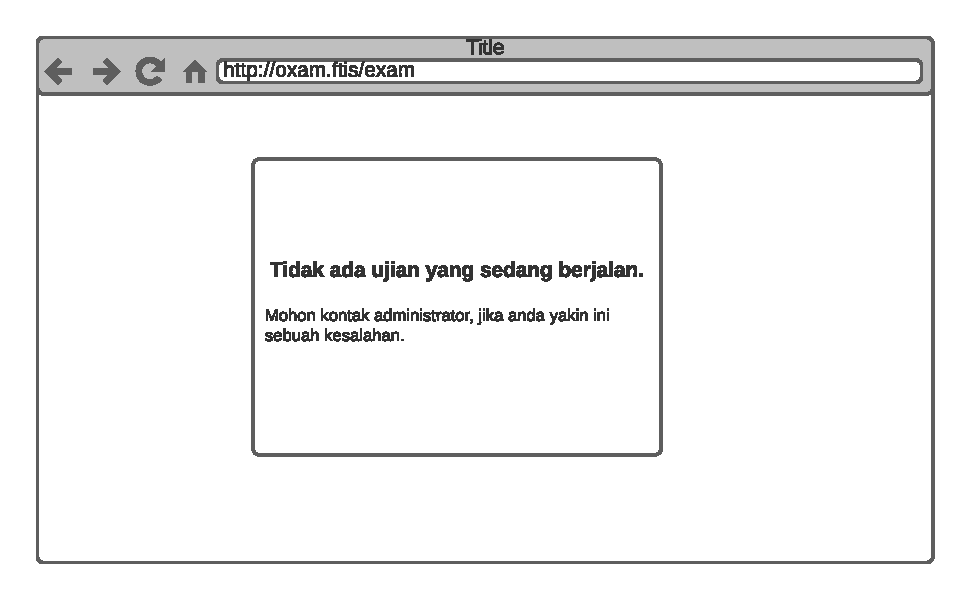
\includegraphics[width=0.7\paperwidth]{Gambar/mockups/Mockup--Peserta - Blankstate.pdf}
        \caption{Rancangan antarmuka untuk peserta, saat ujian sedang tidak berjalan.}
        \label{fig:mockup_peserta_blankstate}
    \end{figure}
     Tampilan antarmuka pertama yang akan dibahas adalah tampilan untuk
     menunjukkan informasi bahwa tidak ada ujian yang sedang berjalan, dapat
     dilihat pada Gambar \ref{fig:mockup_peserta_blankstate}. Hal ini
     diperuntukkan untuk membantu tim admin melakukan pengecekan lebih cepat
     karena tampilan layar yang beda secara signifikan. Selain itu, tampilan
     pesan yang cukup ramah untuk pengguna menampilkan informasi bahwa mungkin
     peserta mengambil tempat duduk yang salah.

    % Screen ujian AKAN mulai
    \begin{figure}[H]
        \centering
        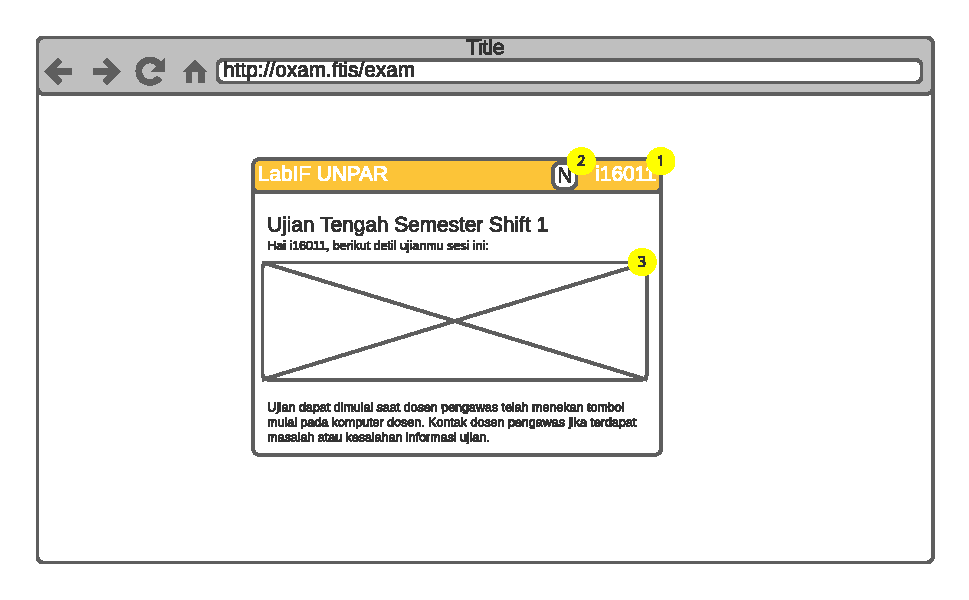
\includegraphics[width=0.7\paperwidth]{Gambar/mockups/Mockup--Peserta - Prestartstate.pdf}
        \caption{Rancangan antarmuka untuk peserta, saat ujian akan berjalan.}
        \label{fig:mockup_peserta_prestartstate}
    \end{figure}
    Rancangan berikutnya adalah tampilan antarmuka untuk memulai ujian, dapat
    dilihat pada \ref{fig:mockup_peserta_prestartstate}. Tampilan ini akan
    ditampilkan pada saat ujian akan dimulai di ruangan. Tampilan ini dibuat
    untuk menahan perserta untuk langsung mengakses lembar jawaban ujian. Pada
    bagian ini terdapat beberapa informasi tentang peserta (poin 1), fitur
    notifikasi untuk mengecek kredensial login lainnya (poin 2), dan informasi
    lengkap ujian dalam bentuk tabel (poin 3). Selain itu terdapat deskripsi
    kecil untuk membantu peserta mengerti konteks dari tampilan layar ini. 
    
    % Screen ujian buka lembar jawab
    \begin{figure}
        \centering
        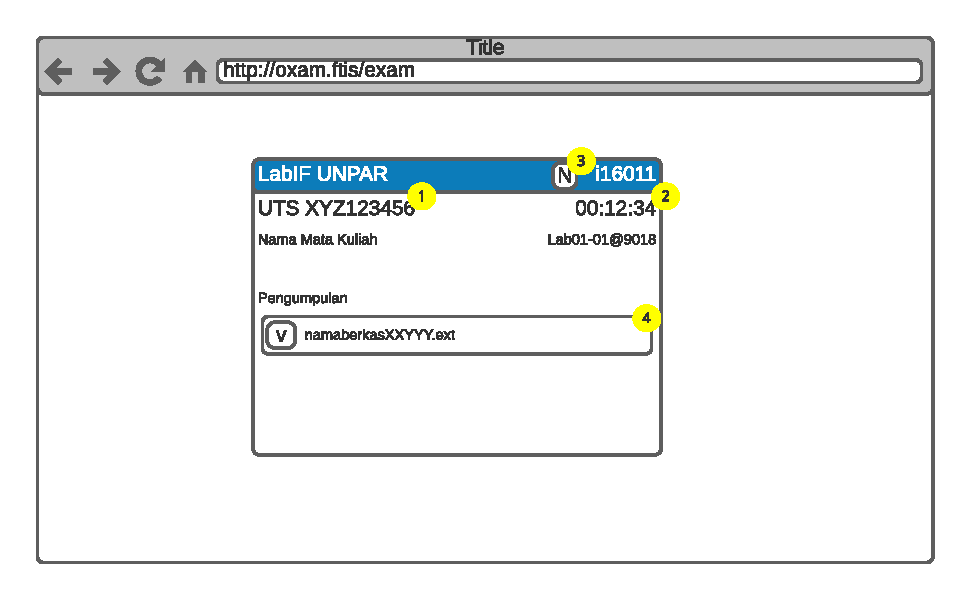
\includegraphics[width=0.7\paperwidth]{Gambar/mockups/Mockup--Peserta - Startstate.pdf}
        \caption{Rancangan antarmuka untuk peserta, saat ujian sedang berjalan.}
        \label{fig:mockup_peserta_activestate}
    \end{figure}
    Antarmuka berikutnya adalah antarmuka saat ujian sedang berjalan, dapat
    dilihat pada Gambar \ref{fig:mockup_peserta_activestate}. Tampilan rancangan
    antarmuka ini memiliki beberapa bagian yang mirip dengan tampilan sebelumnya
    seperti bagian kepala (poin 3), namun dilengkapi dengan informasi singkat
    tentang ujian (poin 1) dan timer ujian serta lokasi tempat duduk (poin 2).
    Selain itu, untuk mempercepat admin melihat status pada layar, bagian kepala
    diwarnai berbeda dengan tampilan sebelumnya (dari kuning menjadi biru).
    
    Bagian yang ditunjukkan oleh poin 4 adalah bagian pengunggahan. Bagian ini
    memiliki informasi tentang nama berkas yang harus dikumpulkan dan tombol
    unggah dan unduh. Tombol unduh akan dapat diklik pada saat peserta berhasil
    mengunggah. Tombol unduh ditambahkan untuk alasan pengecekkan. Berdasarkan
    survei lapangan, peserta biasanya akan diarahkan untuk melakukan pengecekkan
    ulang. Pengencekan tersebut melibatkan peserta untuk mengunduh berkas ujian
    untuk kemudian dipastikan apakah berkas jawaban tersebut sudah sesuai dengan
    apa yang mereka kirimkan.
    
    % Screen ujian notifikasi
    \begin{figure}
        \centering
        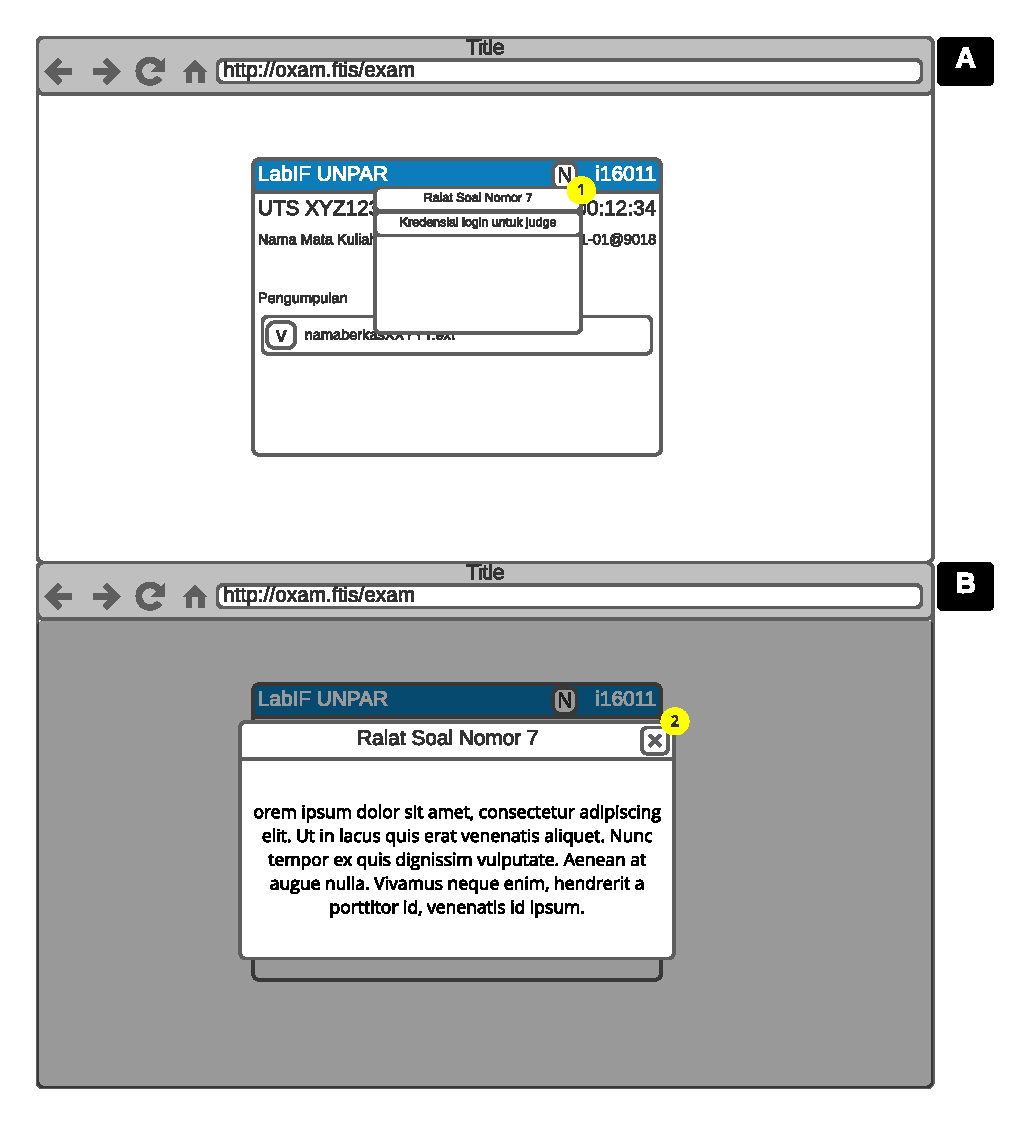
\includegraphics[width=0.7\paperwidth]{Gambar/mockups/Mockup--Peserta - Notif.pdf}
        \caption{Rancangan antarmuka keseluruhan untuk notifikasi
        peserta. \\
            (A) Daftar notifikasi; (B) Notifikasi terbuka.}
        \label{fig:mockup_peserta_notif}
    \end{figure}
    Rancangan berikutnya adalah fitur notifikasi. Fitur ini akan dimuncuklkan
    sejak tahap ujian sedang akan dimulai. Pada Gambar
    \ref{fig:mockup_peserta_prestartstate} dan
    \ref{fig:mockup_peserta_activestate} dapat dilihat bahwa terdapat tombol
    dengan lambang 'N' dekat dengan informasi singkat peserta. tombol tersebut
    adalah tombol notifikasi. Jika tombol tersebut diklik, maka akan tampil
    sebuah daftar notifikasi dalam bentuk \textit{dropdown} (Perhatikan Gambar
    \ref{fig:mockup_peserta_notif}, bagian A). Pada rancangan tampilan, peserta
    dapat melihat beberapa notifikasi yang telah diberikan untuk peserta
    tersebut (perhatikan Poin 1). Jika Poin 1 diklik, maka notifikasi akan
    ditampilkan secara modal (Perhatikan Gambar \ref{fig:mockup_peserta_notif},
    bagian B). Tampilan interaktif dengan modal dipilih untuk menunjukan bahwa
    peserta dapat menutup modal tersebut tanpa kehilangan formulir lembar
    pengumpulan jawaban ujian. Selain itu dengan menggunakan modal, tataletak
    yang sudah ada tidak berubah, dan memperkecil \textit{learning curve} untuk
    peserta membiasakan diri dengan aplikasi ini.
    
    \begin{figure}
        \centering
        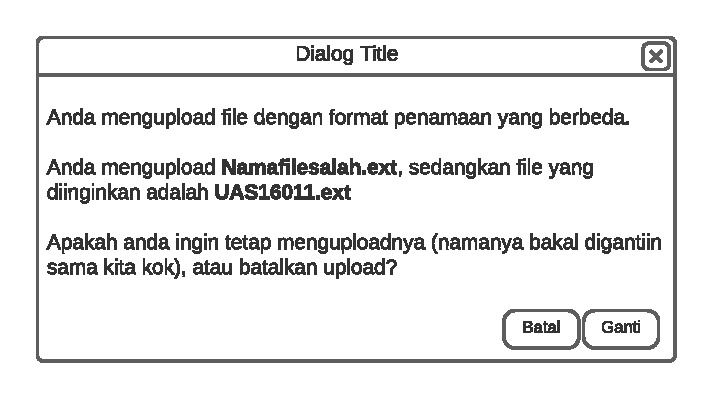
\includegraphics{Gambar/mockups/Mockup--Peserta - Mismatch Filename.pdf}
        \caption{Rancangan tampilan untuk pengumpulan jawaban dengan nama berkas yang tidak sesuai.}
        \label{fig:mockup_peserta_mismatch}
    \end{figure}
    Rancangan antarmuka lainnya adalah tampilan pesan peringatan pengubahan nama
    berkas untuk peserta pada saat peserta mengirimkan berkas dengan nama yang
    tidak sesuai. Sistem akan mengkonfirmasi peserta untuk mengganti nama berkas
    sebelum menunggah berkas ke server. Rancangan tersebut dapat dilihat pada
    Gambar \ref{fig:mockup_peserta_mismatch}.
    
\subsection{Rancangan Antarmuka untuk Admin}
    
    % Screen admin login
\subsubsection{Otentikasi}
    \begin{figure}
        \centering
        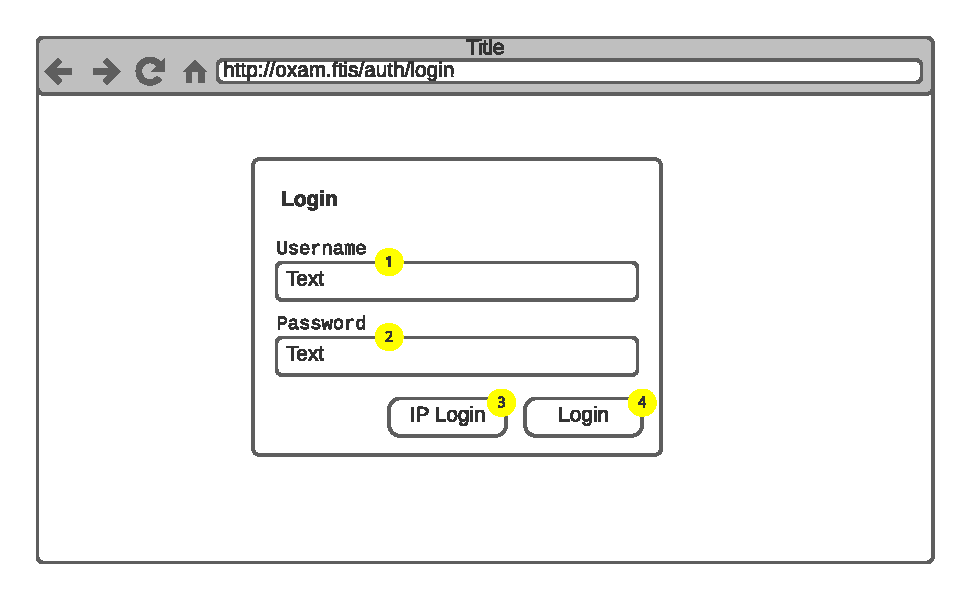
\includegraphics[width=0.7\paperwidth]{Gambar/mockups/Mockup--Admin - Login.pdf}
        \caption{Rancangan antarmuka untuk halaman otentikasi untuk Admin.}
        \label{fig:mockup_admin_login}
    \end{figure}
    Untuk dapat mengakses halaman admin panel, pengguna diharuskan untuk
    melakukan otentikasi terlebih dahulu. Rancangan tampilan admin panel
    tersebut dapat dilihat pada Gambar \ref{fig:mockup_admin_login}. Pada
    rancangan tampilan, terdapat beberapa bagian yang dapat pengguna isi untuk
    login. Bagian yang ditunjukan oleh poin 1 adalah bidang username dari admin.
    Bidang ini rancang untuk dapat menerima namapengguna dan email. Lalu
    bagian berikutnya adalah bidang yang ditunjukkan oleh poin 2. Bidang
    tersebut adalah bidang kata sandi. Lalu pada bagian yang ditunjukan oleh
    poin 3 dan 4 adalah tombol aksi untuk melakukan login. Tombol yang
    ditunjukkan oleh poin 3 tidak memanfaatkan bidang namapengguna dan kata
    sandi, namun akan langsung melakukan pemanggilan API ke backend untuk
    melakukan otentikasi secara nir-kata sandi dengan bantuan IP. Proses ini
    akan dijelaskan lebih lanjut pada bagian rancangan antarmuka untuk dosen
    pengawas. Bagian yang ditunjukkan pada poin 4 adalah tombol login
    sesungguhnya. Pengguna yang telah dipastikan sebagai admin akan dapat
    melakukan login dan diarahkan menuju daftar ujian. Namun jika pengguna
    memasukkan kredensial login yang salah sebuah pesan kesalahan akan
    dimunculkan dalam bentuk \textit{Alert}.
    
\subsubsection{Daftar Ujian}
    % Screen admin exam listing
    \begin{figure}
        \centering
        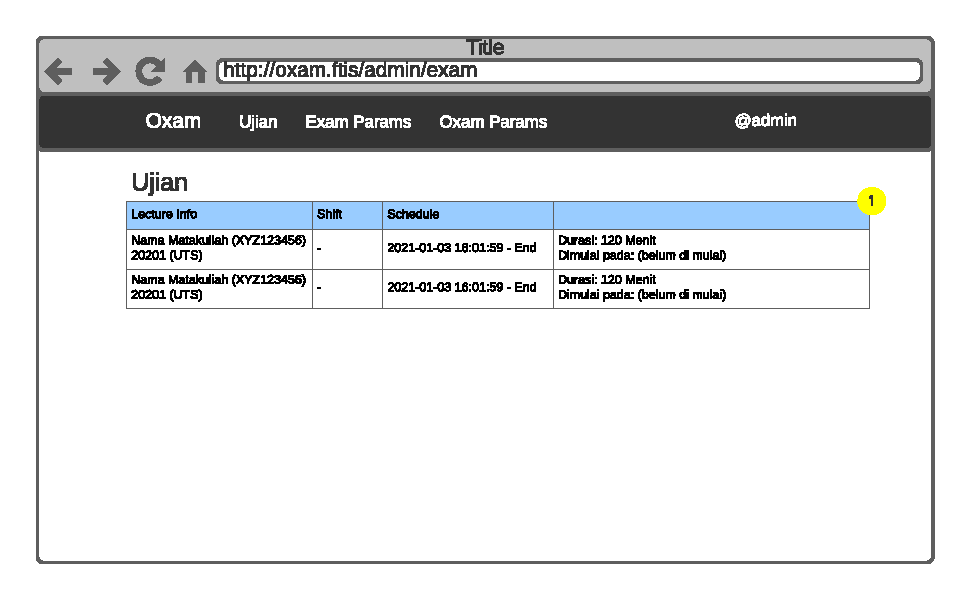
\includegraphics{Gambar/mockups/Mockup--Admin - Exam Listing.pdf}
        \caption{Rancangan antarmuka untuk daftar ujian pada halaman Admin Panel.}
        \label{fig:mockup_admin_exam_listing}
    \end{figure}\begin{figure}
        \centering
        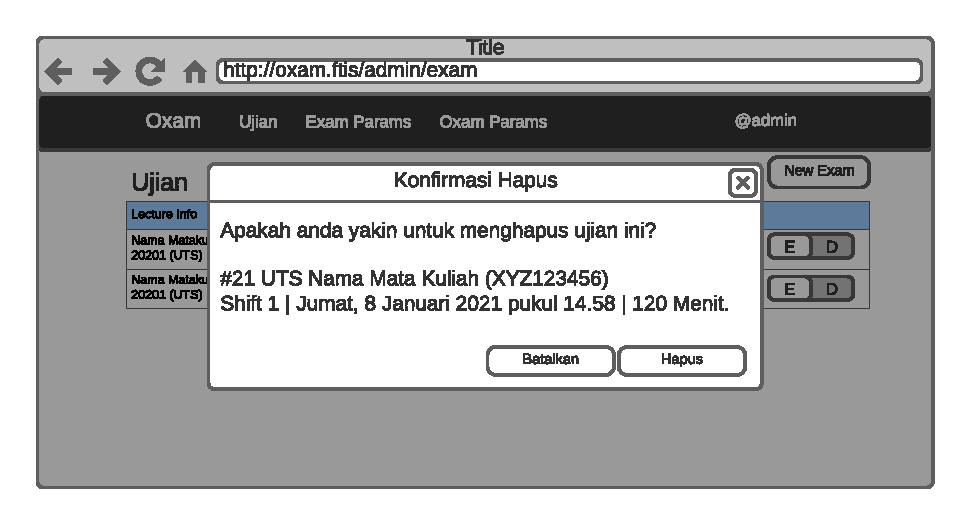
\includegraphics{Gambar/mockups/Mockup--Admin - Exam Delete.pdf}
        \caption{Rancangan antarmuka untuk modal konfirmasi penghapusan ujian.}
        \label{fig:mockup_admin_exam_listing-delete}
    \end{figure}
    Rancangan antarmuka untuk manajemen ujian dimulai dengan halaman daftar
    ujian, dapat dilihat pada Gambar \ref{fig:mockup_admin_exam_listing}. Pada
    rancangan tersebut secara garis besar menampilkan informasi tentang
    ujian-ujian yang sudah terdaftar pada sistem berserta informasi singkatnya.
    Bagian-bagian yang ditunjukkan dengan poin dijelaskan sebagai berikut:
    \begin{itemize}
        \item Bagian yang ditunjukkan pada Poin 1 adalah daftar ujian yang sudah
            teregistrasi pada sistem. Daftar tersebut disajikan dalam bentuk
            tabel yang kemudian dapat diklik untuk menuju halaman detil ujian.
            Tabel akan menunjukan setidaknya informasi mata kuliah, periode
            ujian, UTS atau UAS, \textit{shift}, serta tanggal dan jam mulai
            serta berakhirnya ujian jika ujian sudah dimulai.
            
            Selain itu setiap tabel akan memiliki tombol lihat dan tombol hapus.
            Tombol hapus akan membuka modal konfirmasi hapus yang dapat dilihat
            pada gambar \ref{fig:mockup_admin_exam_listing-delete}. Modal akan
            menampilkan informasi singkat ujian yang akan dihapus untuk
            konfirmasi. 
        
        \item Bagian yang ditunjukkan pada Poin 2 adalah tombol aksi untuk
            membuat ujian yang baru.
    \end{itemize}
    
\subsubsection{Pembuatan Ujian Baru}
    % Screen admin exam create (3-4 screens)
    \begin{figure}
        \centering
        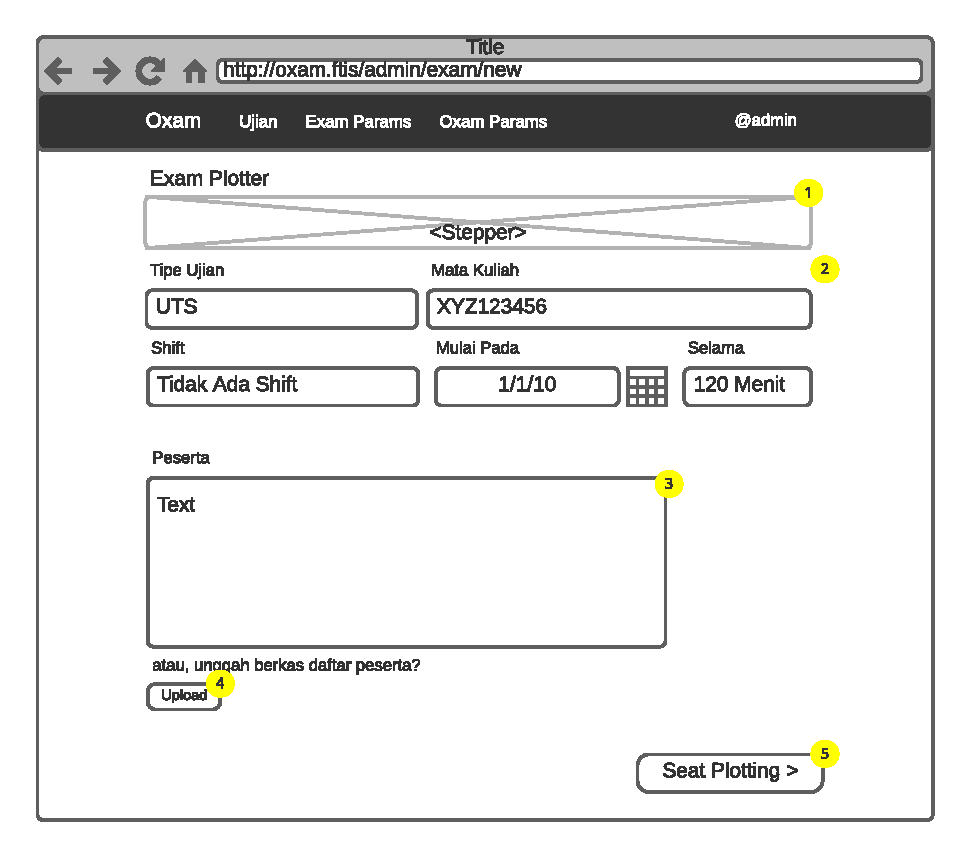
\includegraphics{Gambar/mockups/Mockup--Admin - NewExam-Step 1.pdf}
        \caption{Rancangan antarmuka untuk membuat ujian baru, langkah pertama dari empat.}
        \label{fig:mockup_admin_exam_create-1}
    \end{figure}
    Untuk mendaftarkan ujian Admin harus mengisi formulir yang disediakan oleh
    sistem. Formulir akan dipisah menjadi beberapa langkah untuk mempermudah
    pengecekan. Fomulir pada langkah pertama dapat dilihat pada Gambar
    \ref{fig:mockup_admin_exam_create-1}. Halaman ini dapat diakses pada saat
    Admin menekan tombol yang ditujukkan oleh poin 2 pada gambar
    \ref{fig:mockup_admin_exam_listing}. Poin-poin yang terdapat pada gambar
    dijelaskan sebagai berikut:
    \begin{itemize}
        \item Poin 1 adalah tampilan \textit{stepper}. \textit{Stepper}
            menunjukan langkah yang harus ditempuh oleh tim admin untuk membuat
            mengisi formulir ini. Untuk saat ini terdapat empat langkah besar
            yang terdiri dari:
                \begin{enumerate}
                    \item Pengisian detil ujian (\textit{Exam Details}).
                    \item Pangalokasian tempat duduk ujian (\textit{Seat
                    Plotting}).
                    \item Konfirmasi (\textit{Confirmation}).
                    \item Penyelesaian (\textit{Finish}).
                \end{enumerate}
            Seperti yang telah dijelaskan, halaman formulir ini berada pada
            tahap pengisian detil ujian.
            
        \item Poin 2 menunjukkan bagian detil ujian seperti tipe ujian yang
            dapat diisi sebagai UTS atau pun UAS, mata kuliah dati ujian ini,
            \textit{shift}, mulai pada tanggal jam berapa, hingga durasi waktu
            ujian. Informasi yang ditampilkan pada bagian ini berhubungan
            langsung dengan entitas \texttt{Exam}. Sesuai dengan jenis
            bidangnya, jika sebuah bidang memiliki pilihan spesifik, maka bidang
            tersebut akan diimplementasi dengan \textit{dropdown}. Sebagai
            contoh bidang tipe ujian hanya akan memiliki pilihan UTS atau pun
            UAS, maka bidang diimplementasi dengan \textit{dropdown} dengan
            nilai pilihan yang sudah disebutkan. Untuk bidang tanggal dan jam,
            implementasi akan dilakukan dengan bantuan dari \textit{date
            picker}.
            
        \item Poin 3 menunjukkan daftar peserta yang akan mengikuti ujian ini.
            Daftar peserta berisi daftar NPM yang mengikuti ujian, dipisah
            dengan sebuah enter.
            
        \item Poin 4 adalah sebuah tombol unggah yang akan diproses langsung
            pada browser untuk memasukkan daftar peserta. Tombol ini ditambahkan
            dengan alasan kompatibilitas UX dengan sistem yang lama.
            
        \item Poin 5 adalah sebuah tombol aksi untuk menuju langkah berikutnya,
            pengalokasian tempat duduk ujian.
        
    \end{itemize}
    
    
    \begin{figure}
        \centering
        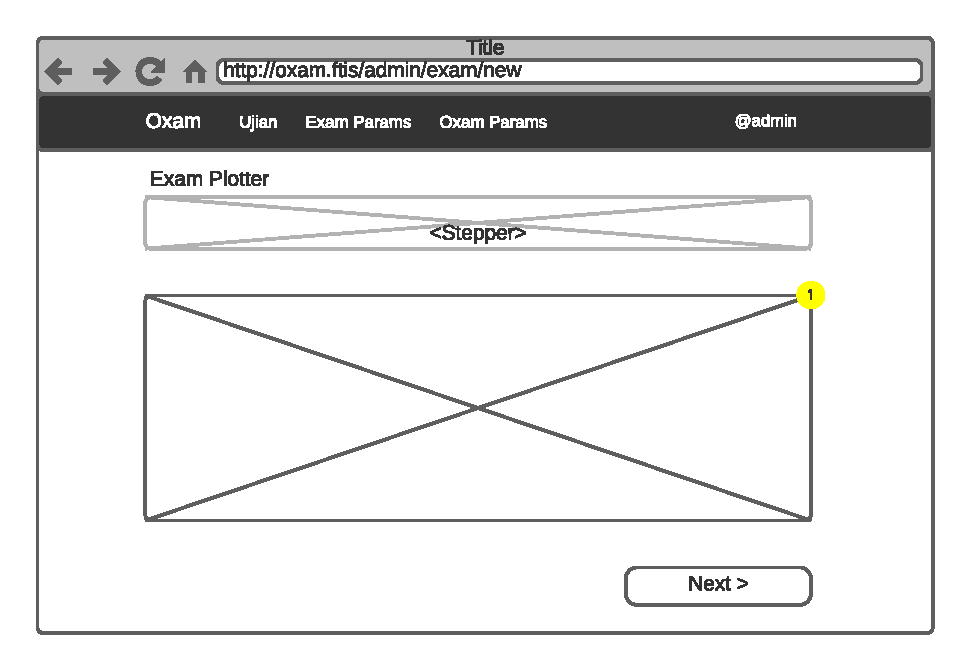
\includegraphics{Gambar/mockups/Mockup--Admin - NewExam-Step 2.pdf}
        \caption{Rancangan antarmuka untuk membuat ujian baru, langkah kedua dari empat.}
        \label{fig:mockup_admin_exam_create-2}
    \end{figure}
    
    Setelah tim admin selesai mengisi informasi detil ujian, maka langkah
    selanjutnya yang akan dilakukan adalah mengalokasi tempat duduk ujian.
    Alokasi ini dilakukan dengan bantuan peta ruangan yang telah didefinisikan
    sebelumnya oleh sistem. Rancangan antarmuka tersebut dapat dilihat pada
    Gambar \ref{fig:mockup_admin_exam_create-2}. Secara garis besar tampilan
    memiliki tataletak yang mirip dengan langkah sebelumnya: Judul langkah
    diatas, diikuti dengan \textit{stepper} di bawahnya. Namun bagian yang
    ditunjukkan pada poin 1 akan berisi peta tempat duduk ruangan. Peta tempat
    duduk ini nantinya akan memiki tampilan yang sama dengan yang ditampilkan
    pada proyektor.
    
    \begin{figure}
        \centering
        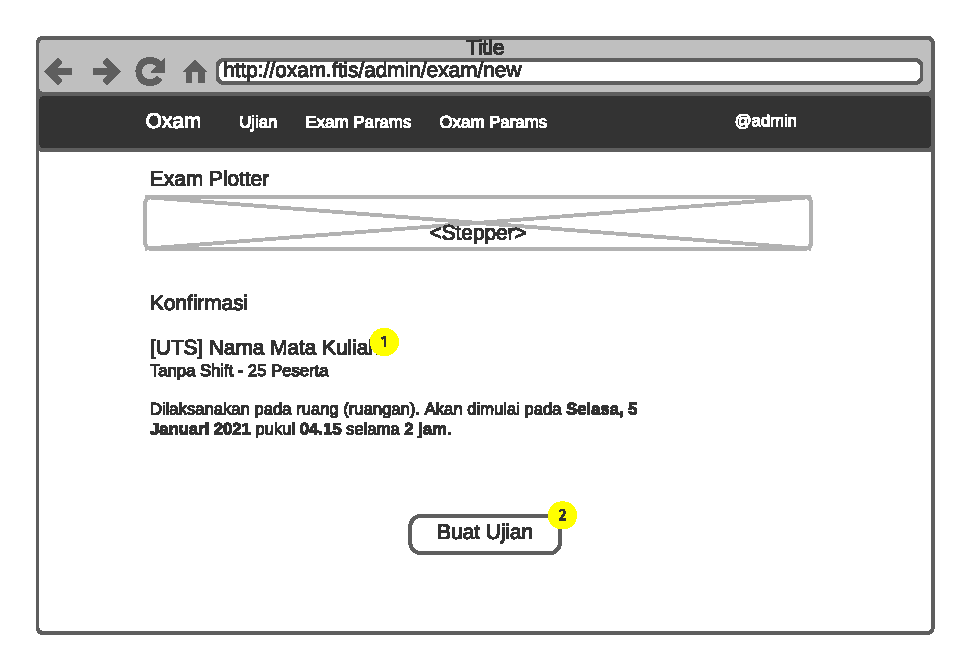
\includegraphics{Gambar/mockups/Mockup--Admin - NewExam-Step 3.pdf}
        \caption{Rancangan antarmuka untuk membuat ujian baru, langkah ketiga dari empat.}
        \label{fig:mockup_admin_exam_create-3}
    \end{figure}
    Setelah tempat duduk dialokasi, langkah berikutnya adalah konfirmasi. Tim
    admin diharapkan untuk mengkonfirmasi detil ujian yang akan dibuat sebelum
    akhirnya difinialisasi oleh sistem. Rancangan tampilan layar tersebut dapat
    diperhatikan pada \ref{fig:mockup_admin_exam_create-3}. Pada rancangan
    tampilan tersebut terdapat informasi singkat dari ujian yang akan dibuat.
    Bagian yang ditunjukkan dengan poin-poin pada gambar akan dijelaskan sebagai
    berikut:
    
    \begin{itemize}
        \item Poin 1 menunjukkan informasi tentang nama matakuliah, banyak
            peserta, informasi shift serta informasi jadwal ujian tersebut.
            
        \item Poin 2 adalah tombol aksi untuk melakukan pembuatan ujian. Tombol
            ini akan melakukan beberapa pemanggilan ke sistem backend sekaligus
            sebelum akhirnya memindahkan tim admin ke tahap berikutnya.
    \end{itemize}
    
    
    \begin{figure}
        \centering
        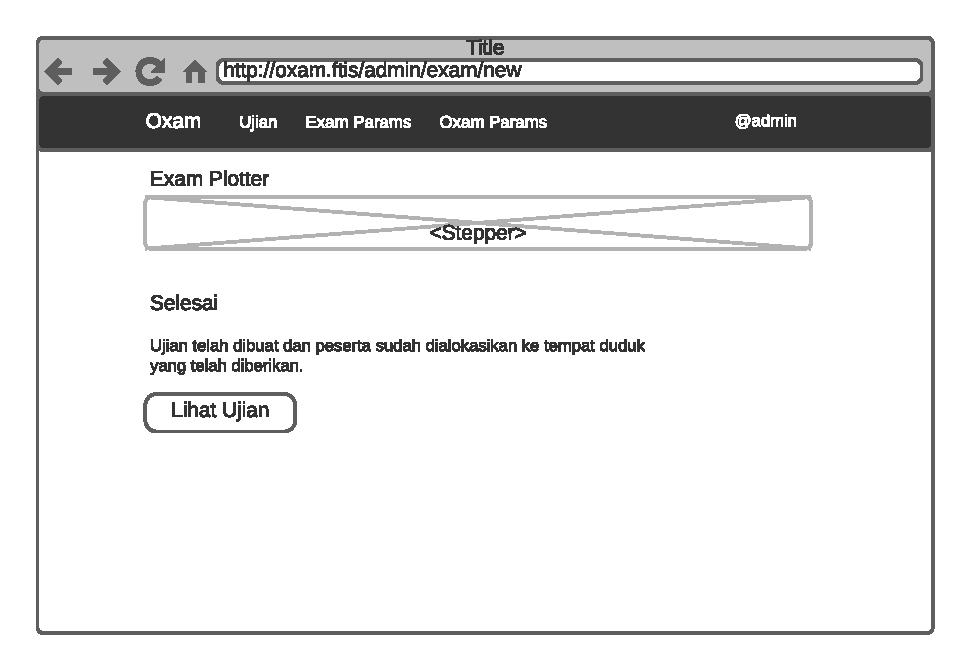
\includegraphics{Gambar/mockups/Mockup--Admin - NewExam-Step 4.pdf}
        \caption{Rancangan antarmuka untuk membuat ujian baru, langkah keempat dari empat.}
        \label{fig:mockup_admin_exam_create-4}
    \end{figure}
    Antarmuka terkahir untuk tahap pembuatan ujian adalah tahap penyelesaian.
    Tampilan antarmuka ini dapat dilihat pada gambar
    \ref{fig:mockup_admin_exam_create-4}. Tampilan ini berfungsi untuk
    menampilkan respon dari sistem bahwa ujian telah berhasil dibuat dengan
    informasi yang telah diberikan. Antarmuka pada tahap ini hanya akan berisi
    pesan respon singkat disertai dengan tombol "Lihat Ujian" tombol ini akan
    mengarahkan tim admin ke halaman ujian.
    
    % Screen admin exam details (mayan banyak)
\subsubsection{Detil Ujian}
    \begin{figure}
        \centering
        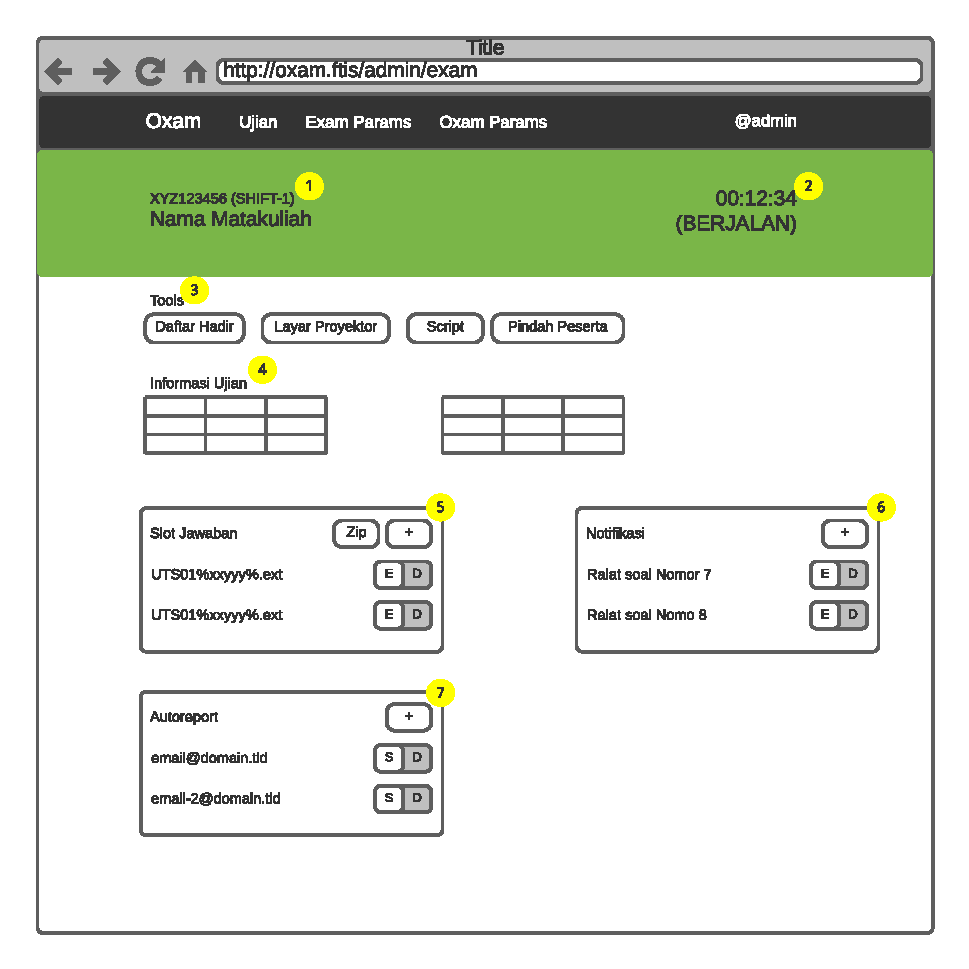
\includegraphics[width=0.75\paperwidth]{Gambar/mockups/Mockup--Admin - Exam Details.pdf}
        \caption{Rancangan antarmuka untuk tampilan detil ujian.}
        \label{fig:mockup_admin_exam_details}
    \end{figure}
    
    \begin{figure}
        \centering
        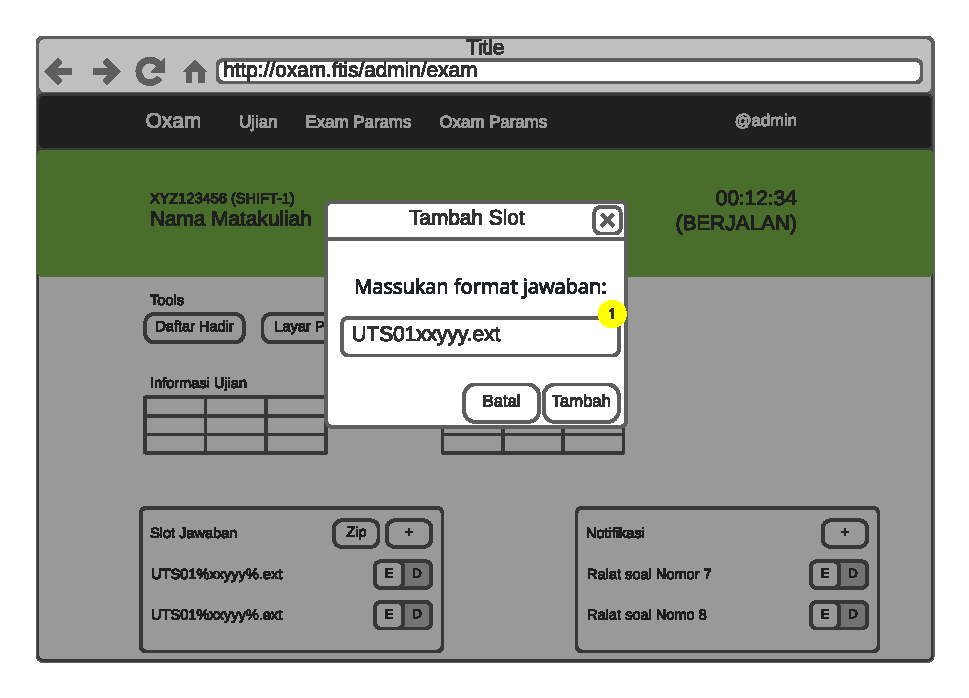
\includegraphics[width=0.75\paperwidth]{Gambar/mockups/Mockup--Admin - Slot Jawaban.pdf}
        \caption{Rancangan antarmuka untuk modal slot jawaban baru.}
        \label{fig:mockup_admin_exam_det_answer_slot}
    \end{figure}
    
    \begin{figure}
        \centering
        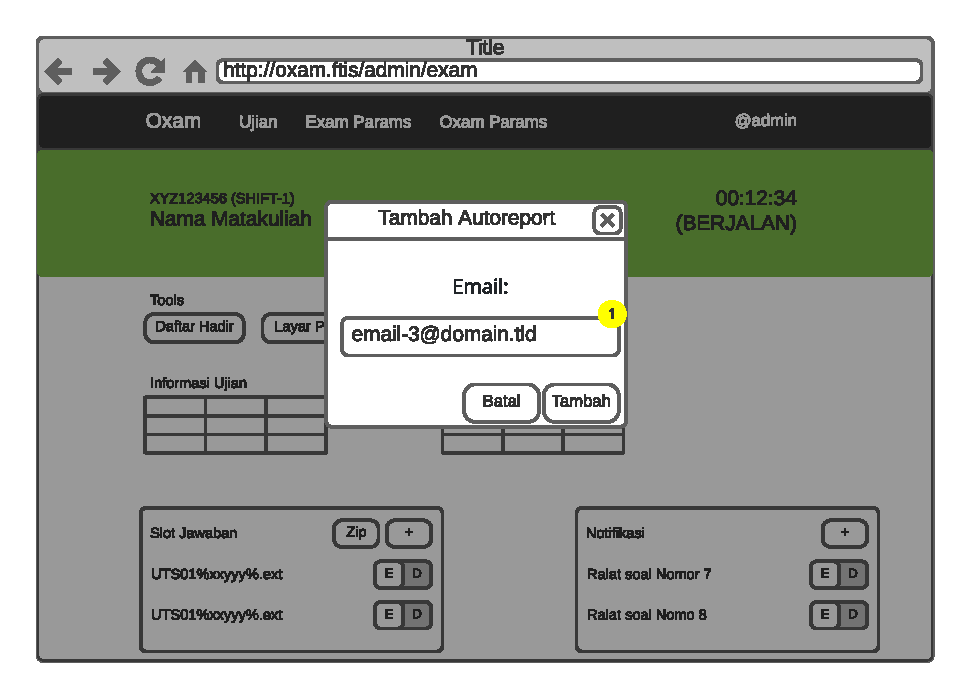
\includegraphics[width=0.7\paperwidth]{Gambar/mockups/Mockup--Admin - Tambah Autoreport.pdf}
        \caption{Rancangan antarmuka untuk modal pelaporan otomatis. \\
            (A) Buat baru. (B) Hapus.}
        \label{fig:mockup_admin_exam_det_autoreport}
    \end{figure}
    
    Halaman detil ujian akan memuat seluruh informasi ujian yang ditampung pada
    entitas \texttt{Exam} dan beberapa entitas lainnya yang terhubung dengan
    entitas ini. Rancangan tampilan detil ujian dapat dilihat pada gambar
    \ref{fig:mockup_admin_exam_details}. Secara garis besar, tampilan memiliki
    beberapa bagian yang spesifik dengan perannya. Hal ini dibuat demikian untuk
    mempermudah tim admin memindai informasi pada saat membuka beberapa
    \textit{tab} pada peramban. Bagian-bagian yang ditunjukkan dengan poin
    berwarna kuning akan dijelaskan sebagai berikut:
    \begin{itemize}
        \item Poin 1 adalah bagian informasi singkat tentang ujian. Informasi
            akan berisi minimal kode mata kuliah, \textit{shift} (jika ada), dan
            nama matakuliah.
            
        \item Poin 2 akan berisi status dari ujian tersebut, serta sisa waktu
            yang ada jika ujian tersebut sedang berjalan.
            
        \item Poin 3 adalah kotak alat untuk ujian ini. Kotak alat tersebut
            terdiri dari beberapa tombol yaitu
            \begin{itemize}
                \item Tombol cetak daftar hadir, untuk pintu, maupun untuk
                absensi.
                \item Tombol layar proyektor.
                \item Tombol unduh \textit{script} untuk membuat folder dan
                berkas ujian.
                \item Tombol pemindahan peserta.
            \end{itemize}
            Kotak alat diimplementasikan untuk memenuhi kebutuhan yang muncul
            dari admin sebelumnya.
            
        \item Poin 4 menunjukkan informasi ujian dengan lebih detil, disajikan
        dalam bentuk tabel.
        
        \item Poin 5 adalah bagian pengelolaan Slot Jawaban. Bagian ini terdiri
        dari beberapa tombol.
            \begin{itemize}
                \item Pada bagian atas, terdapat tombol Zip yang digunakan untuk
                    melakukan pengumpulan berkas jawaban menjadi sebuah
                    \textit{archive} zip. Peramban akan kemudian mengunduh
                    berkas tersebut dan tim admin dapat mengirimkan berkas
                    jawaban tersebut secara manual ke dosen.
                    
                \item Pada sebelah kanan tombol Zip, terdapat tombol tambah yang
                    akan membuka sebuah modal yang akan menanyakan format slot
                    jawaban yang ada. Modal tersebut dapat dilihat pada Gambar
                    \ref{fig:mockup_admin_exam_det_answer_slot} Bagian A. Pada
                    poin 1 dari Gambar
                    \ref{fig:mockup_admin_exam_det_answer_slot}, format yang
                    diterima dapat berupa format \textit{xxyyy} seperti pada
                    sistem sebelummnya.
                    
                \item Untuk setiap slot jawaban yang ada, akan terdapat tombol
                    ubah untuk mengubah lembar jawab, dan tombol hapus yang
                    dapat digunakan untuk menghapus entri tersebut. Tombol hapus
                    tersebut akan membuka modal konfirmasi seperti pada Gambar
                    \ref{fig:mockup_admin_exam_det_answer_slot}. Modal akan
                    menampilkan informasi slot ujian dan tombol aksi.
            \end{itemize}
            
        \item Poin 6 menunjukkan bagian fitur notifikasi yang akan ditampilkan
            pada peserta ujian. Pada tampilan ini, terdapat beberapa tombol yang
            dapat digunakan untuk memanipulasi ujian tersebut. Tombol-tombol
            tersebut terdiri dari
                \begin{itemize}
                    \item Tombol Tambah untuk membuat notifikasi baru. Pada saat
                        diklik, sistem akan menampilkan sebuah modal yang
                        menanyakan informasi jenis notifikasi. Karena alur yang
                        cukup panjang, alur kerja untuk pembuatan notifikasi
                        akan dibahas setelah bagian ini.
                        
                    \item Untuk setiap entri notifikasi akan memiliki dua buah
                        tombol yang dapat digunakan untuk mengubah dan menghapus
                        entri tersebut.
                \end{itemize}
            
        \item Poin 7 menunjukan bagian fitur pelaporan otomatis. Fitur pelaporan
            otomatis ini memiliki beberapa tombol aksi seperti:
           \begin{itemize}
               \item Tombol Tambah yang dapat digunakan untuk menambahkan
                    autoreport baru. Jika tombol ini diklik, sistem akan
                    memunculkan modal yang menanyakan pada siapa report ini akan
                    dikirimkan. rancangan modal tersebut dapat dilihat pada
                    Gambar \ref{fig:mockup_admin_exam_det_autoreport}. Bagian
                    yang ditunjukan pada poin 1 dari rancangan tersebut dapat
                    diisi dengan daftar email yang dipisah dengan tanda koma.
                    
                \item Untuk setiap entri pada bagian ini memiliki dua tombol
                    yang dapat digunakan untuk mengirimkan email, dan
                    penghapusan entri. Tombol penghapusan entri akan menampilkan
                    modal konfirmasi penghapusan, seperti yang dapat dilihat
                    pada Gambar \ref{fig:mockup_admin_exam_det_autoreport}.
                    Modal tersebut akan menampilkan informasi singkat tentang
                    entri yang ada dan tombol aksi.
           \end{itemize}
    \end{itemize}
    
\subsubsection{Detil Ujian: Fitur notifikasi}
    \begin{sidewaysfigure}
        \centering
        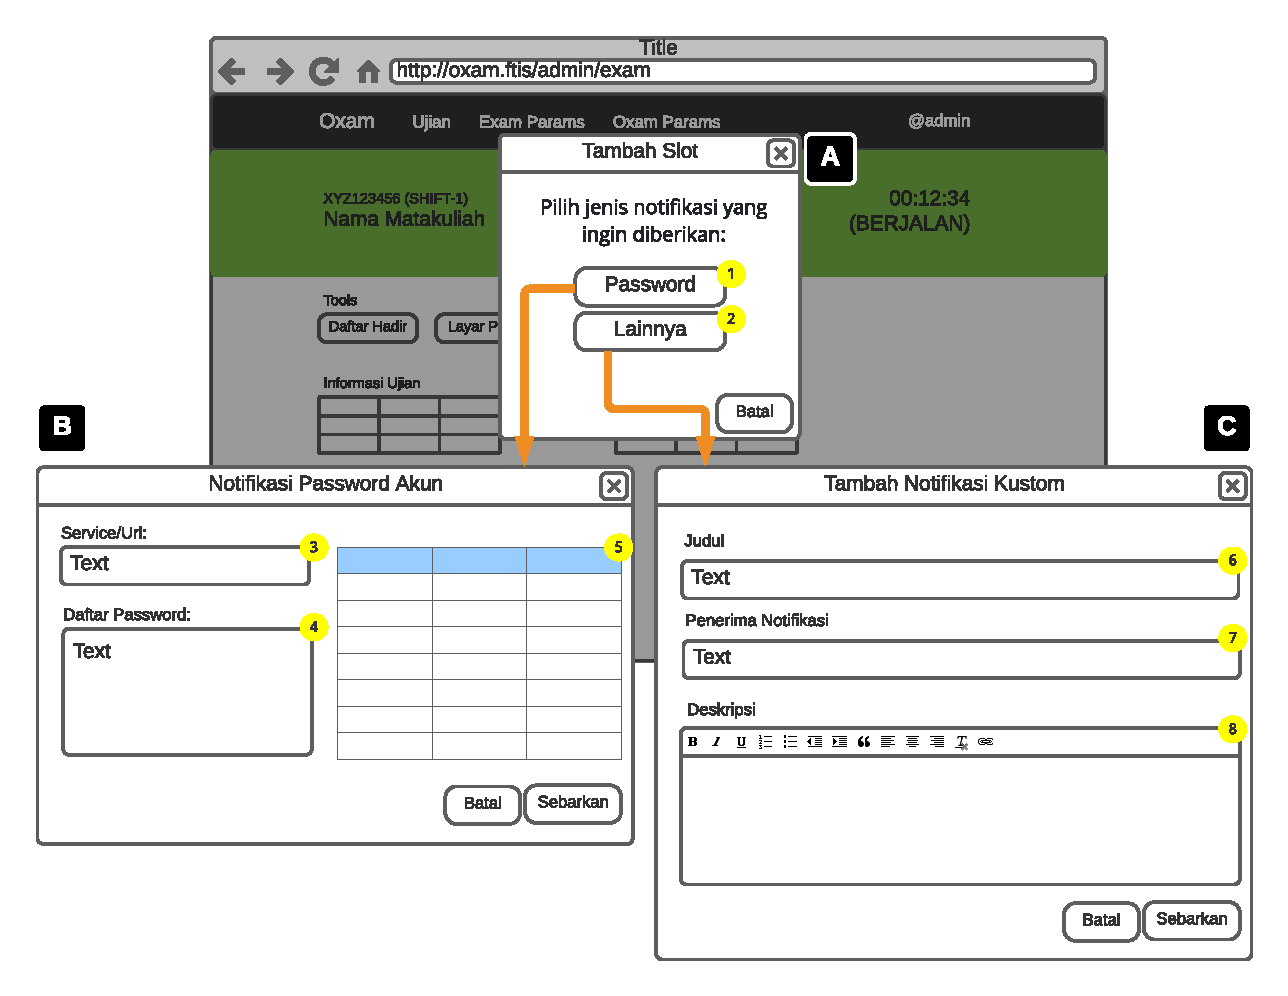
\includegraphics{Gambar/mockups/Mockup--Admin - Notif.pdf}
        \caption{Rancangan antarmuka untuk beberapa tampilan modal jenis
        notifikasi. \\
            (A) Modal jenis notifikasi; (B) Notifikasi Kata Sandi; (C)
            Notifikasi Lainnya.}
        \label{fig:mockup_admin_exam_det_notif}
    \end{sidewaysfigure}
    
    Pada bagian notifikasi, rancangan tampilan antarmuka memiliki beberapa
    bagian tergantung dari jenis notifikasi yang ingin disebarkan ke setiap
    peserta. Seperti yang dapat dilihat pada
    \ref{fig:mockup_admin_exam_det_notif}, rancangan tampilan antarmuka terdapat
    tiga bagian.
    
    Bagian yang ditunjukan dengan label A adalah modal pertama yang muncul pada
    saat tim admin menekan tombol tambah. Modal akan memiliki dua buah tombol
    yang merepresentasikan jenis yang didukung oleh fitur ini: Kata sandi (poin
    1) dan lainnya (poin 2). Jika tombol untuk jenis kata sandi dipilih, maka
    tim admin akan disajikan modal dengan label B. Sebaliknya, jika tombol untuk
    jenis lainnya dipilih, maka sistem akan menyajikan modal dengan label C.
    
    Modal yang ditunjukkan dengan label B adalah modal untuk mengisi informasi
    layanan dan daftar kata sandi yang akan disebarkan. Bagian-bagian yang
    terdapat pada modal ini adalah sebagai berikut
    \begin{itemize}
        \item Poin 3 menunjukan informasi tentang layanan dari kata sandi yang
            akan disebar.
        
        \item Poin 4 adalah daftar kata sandi dalam bentuk teks yang berisi
            informasi namapengguna dan kata sandi, serta npm yang dipisah dengan
            karakter enter untuk setiap entrinya.
            
        \item Poin 5 adalah tabel daftar peserta yang akan menerima kredensial
            nama pengguna dan kata sandi dari tim admin. Tabel ini ditambahkan
            untuk tim admin melakukan pengecekan sebelum notifikasi disebar.
    \end{itemize}
    
    Kemudian, modal yang ditunjukkan dengan label C adalah modal untuk jenis
    notifikasi lainnya. Notifikasi ini nantinya akan dapat ditargetkan untuk
    peserta-peserta tertentu. Bagian-bagian yang terdapat pada modal ini
    dijelaskan sebagai berikut
    \begin{itemize}
        \item Poin 6 menunjukan bidang judul yang akan disampaikan ke peserta
        ujian.
        
        \item Poin 7 menunjukan bidang yang digunakan untuk mespesifikasikan
        penerima notifikasi ujian.
        
        \item Poin 8 adalah isi dari notifikasi tersebut.
    \end{itemize}
    
    
    \begin{figure}
        \centering
        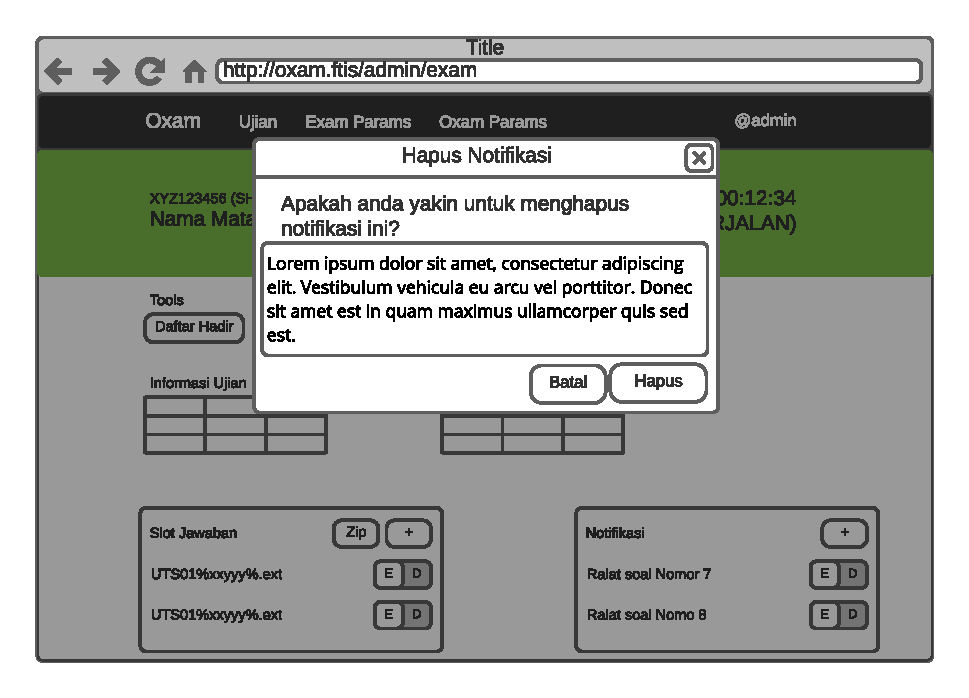
\includegraphics{Gambar/mockups/Mockup--Admin - Notif Delete.pdf}
        \caption{Rancangan antarmuka untuk modal konfirmasi penghapusan notifikasi.}
        \label{fig:mockup_admin_notif_delete}
    \end{figure}
    Untuk menghapus notifikasi ujian, tim admin dapat menekan tombol yang
    nantinya akan menampilkan modal untuk konfirmasi penghapusan. Rancangan
    tampilan modal tersebut dapat diperhatikan pada Gambar
    \ref{fig:mockup_admin_notif_delete}. Modal akan menampilkan informasi badan
    notifikasi dan tombol aksi.
    
    
    % Absensi (pintu dan tanda tangan)
\subsubsection{Detil Ujian: Daftar Hadir}
    \begin{figure}
        \centering
        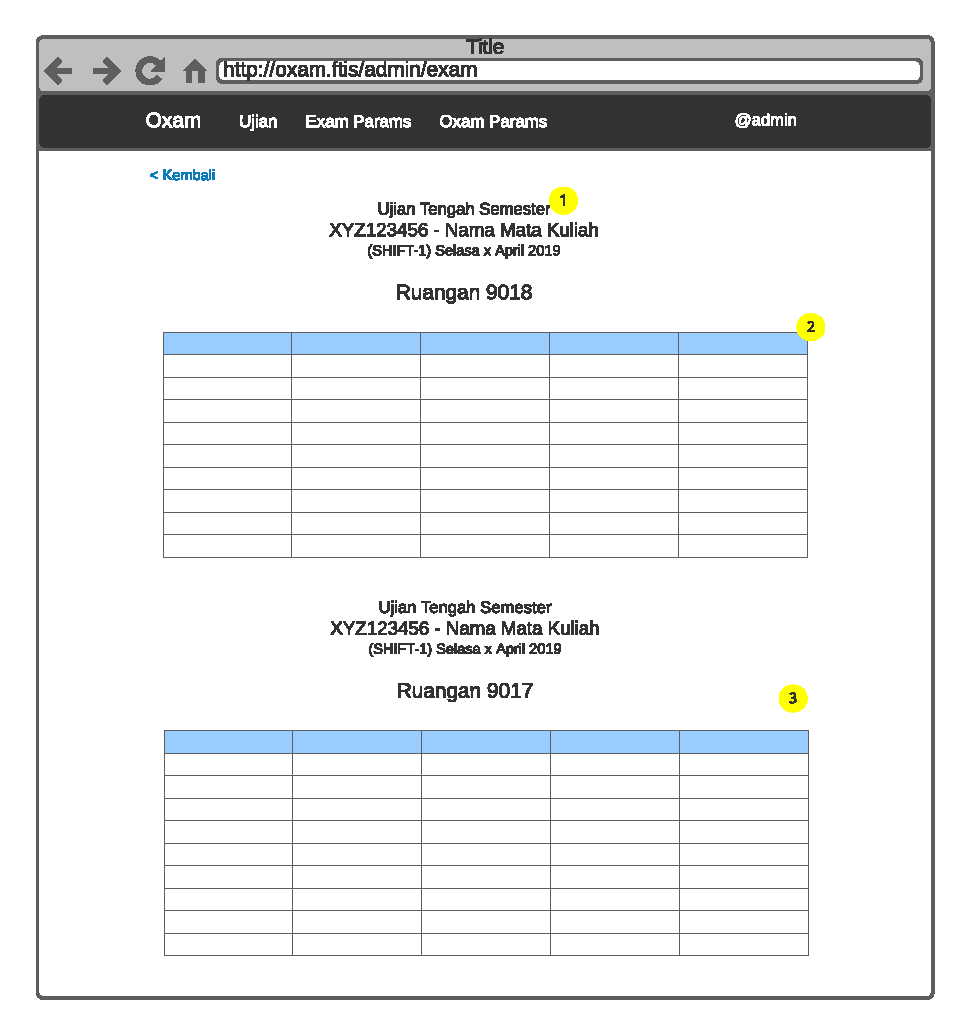
\includegraphics{Gambar/mockups/Mockup--Admin - Daftar Hadir.pdf}
        \caption{Rancangan tampilan untuk daftar hadir peserta ujian.}
        \label{fig:admin_mockup_exam_det_daftar-hadir}
    \end{figure}
    
    Salah satu bagian dari kotak alat yang disediakan untuk tim admin adalah
    daftar hadir. Rancangan tampilan daftar harid dapat dilihat pada Gambar
    \ref{fig:admin_mockup_exam_det_daftar-hadir}. Daftar hadir tersebut harus
    dapat dicetak dengan pencentak. Daftar hadir ini akan terdiri dari sebuah
    halaman yang berisi beberapa bagian penting, seperti
    \begin{itemize}
        \item Poin 1, informasi singkat ujian seperti informasi UTS/UAS, kode
            mata kuliah, nama mata kuliah, shift (jika ada), tanggal mulai, dan
            ruangan.
        
        \item Poin 2, daftar peserta dengan pengurutan kolom tertentu. Jika
            daftar hadir ditempelkan pada pintu, maka daftar hadir harus
            diurutkan berdasarkan NPMnya. Jika daftar hadir digunakan untuk
            absensi, maka daftar tersebut harus diurutkan berdasarkan nomor
            komputernya.
            
        \item Poin 3, daftar hadir pada ruangan lain yang setiap daftar hadirnya
            terdiri dari poin 1 dan 2. Daftar hadir ini harus dapat terpisah
            menjadi halaman baru pada saat dicetak.
    \end{itemize}
    
    Tampilan daftar hadir ini harus dapat dicetak oleh pencetak atau
    \textit{printer}. Sehingga setiap halaman harus memiliki logo UNPAR dan
    informasi fakultas.
    
    % Timer
\subsubsection{Detil Ujian: Layar Proyektor}
    \begin{figure}
        \centering
        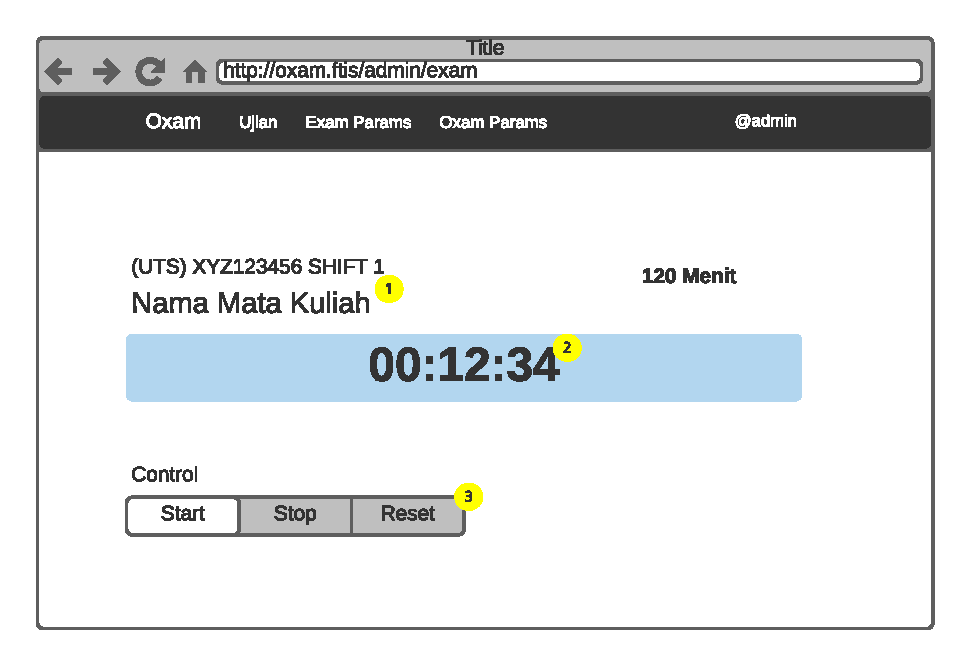
\includegraphics{Gambar/mockups/Mockup--Admin - Layar Proyektor.pdf}
        \caption{Rancangan antarmuka untuk tampilan pada layar proyektor.}
        \label{fig:mockup_admin_det_projector}
    \end{figure}
    
    % TODO: Ganti wording.
    Fitur berikutnya adalah tampilan timer untuk proyektor. Rancangan tampilan
    dapat dilihat pada Gambar \ref{fig:mockup_admin_det_projector}. Karena akun
    admin tidak memiliki relasi dengan lokasi ruangan, maka tampilan ini
    ditambahkan sebagai cadangan dan digunakan hanya pada saat darurat. Tampilan
    ini akan memiliki informasi singkat tentang ujian yang akan diadakan dan
    durasinya (poin 1), sisa waktu (poin 2) dan tombol kontrol timer (poin 3).
    Tombol kontrol timer ini akan terhubung dengan sistem untuk membuka dan
    menutup lembar jawab.
    

    % Pindah
\subsubsection{Detil Ujian: Pindah Peserta}
    \begin{figure}
        \centering
        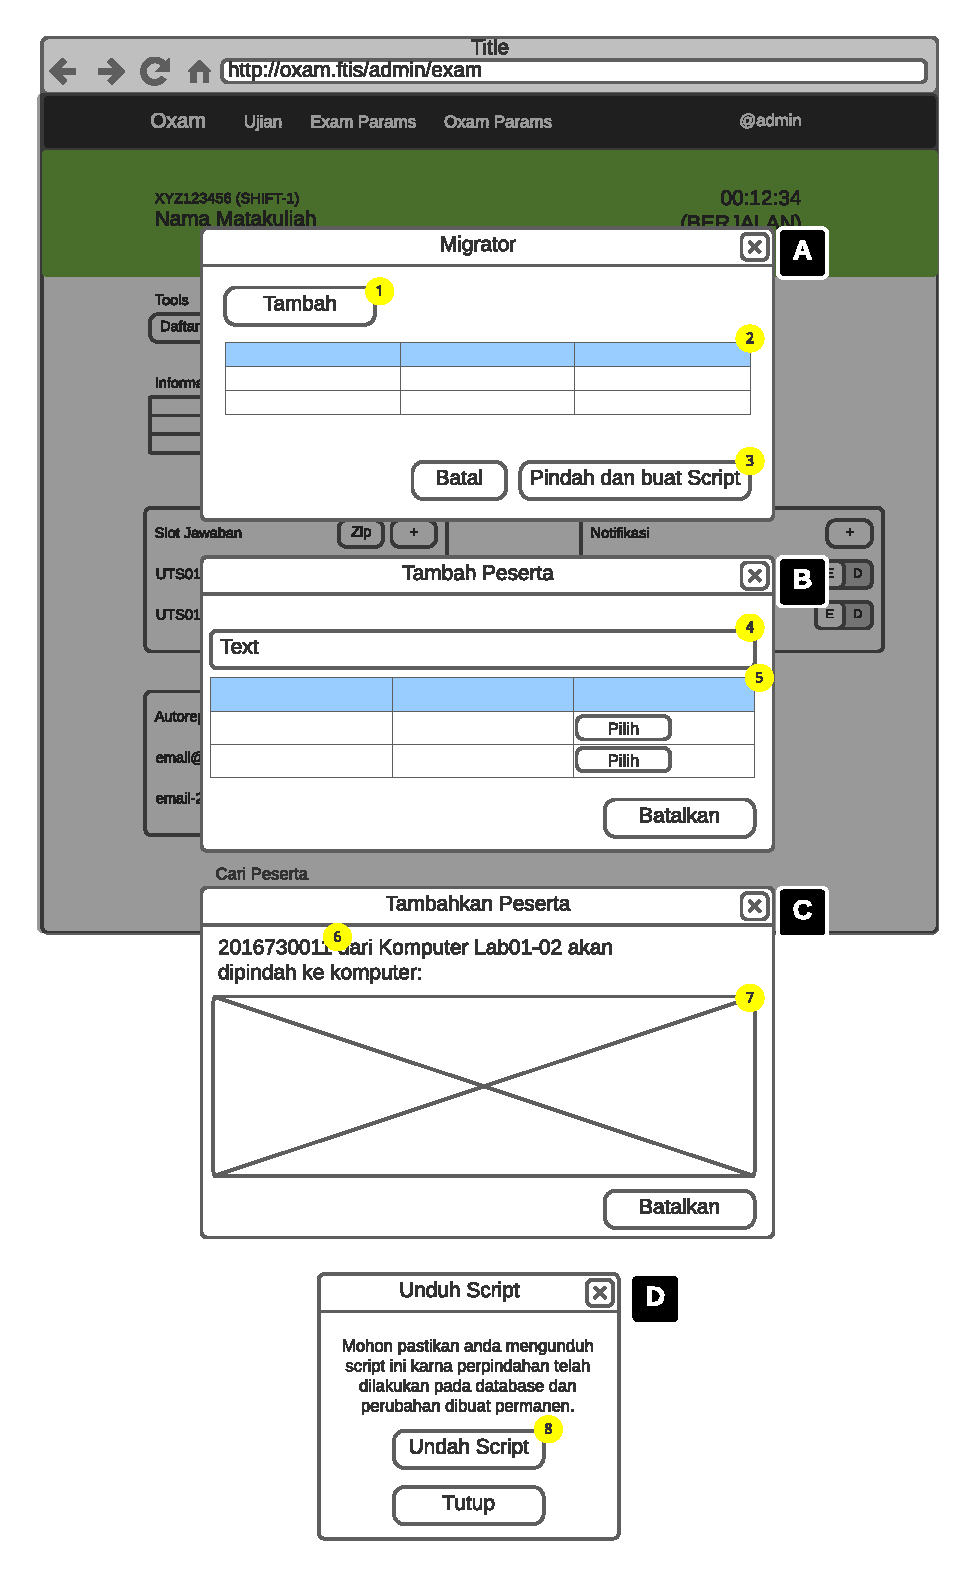
\includegraphics[height=0.7\paperheight]{Gambar/mockups/Mockup--Admin - Pindah Peserta.pdf}
        \caption{Rancangan tampilan untuk pemindahan peserta. \\
            (A) Daftar pemindahan; (B) Pencari peserta target; (C) Pencari
            komputer target; (D) Konfirmasi dan pengunduhan \textit{script}
            pemindahan.}
        \label{fig:mockup_admin_exam_det_migrator}
    \end{figure}
    
    Fitur pada kotak alat berikutnya adalah fitur untuk memindahkan peserta.
    Rancangan tampilan pada fitur ini dapat dilihat pada Gambar
    \ref{fig:mockup_admin_exam_det_migrator}. Fitur pemindahan ini akan melalui
    tahapan seperti memilih peserta yang akan dipindahkan (Bagian B), memilih
    komputer tujuan (Bagian C), lalu eksekusi script yang diberikan oleh sistem
    (Bagian D). Poin-poin yang ditujukkan pada sistem akan dijelaskan sebagai
    berikut:
    \begin{itemize}
        \item Modal Migrator (Bagian A)
            \begin{itemize}
                \item Poin 1 adalah tombol tambah yang akan membuka Modal yang
                    terdapat pada bagian B.
                
                \item Poin 2 menunjukkan daftar peserta yang akan dipindahkan
                    beserta komputer tujuannya.
                
                \item Poin 3 adalah tombol eksekusi pemindahan pada level basis
                    data dan bangkitkan sebuah \textit{script} untuk melakukan
                    pemindahan lembar kerja peserta.
            \end{itemize}
        
        \item Modal Tambah Peserta (Bagian B)
            \begin{itemize}
                \item Poin 4 adalah bidang pencarian cepat untuk membantu tim
                    admin mencari peserta yang ingin dipindah.
                    
                \item Poin 5 menunjukkan daftar peserta yang terdapat pada ujian
                    ini, dengan sebuah tombol pilih pada tiap entri untuk
                    memilih peserta bersangkutan untuk melakukan pemindahan.
            \end{itemize}
            
        \item Modal Pilih Komputer (Bagian C)
            \item Poin 6 menunjukkan informasi peserta mana yang akan dipindah.
                Bagian ini ditambahkan untuk menyakinkan admin bahwa admin telah
                memilih peserta yang benar.
                
            \item Poin 7 adalah peta tempat duduk ujian pada ruangan tertentu.
                Komputer pada peta tersebut dapat diklik untuk dipilih. Saat
                tempat duduk selesai dipilih, maka modal akan kembali ke Bagian
                A, hingga seluruh peserta yang ingin dipindah telah didaftarkan
                seluruhnya.
    \end{itemize}
    
    % Tampilan mobile (minipanel)
\subsubsection{Detil Ujian: Minipanel}
    \begin{figure}
        \centering
        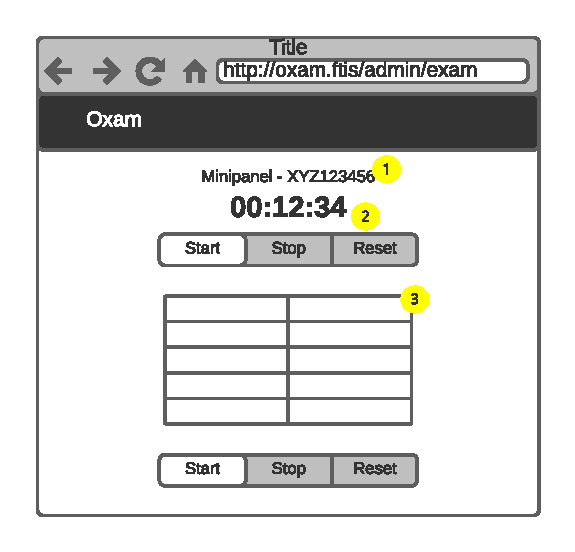
\includegraphics{Gambar/mockups/Mockup--Admin - Minipanel.pdf}
        \caption{Rancangan antarmuka untuk Minipanel.}
        \label{fig:mockup_admin_minipanel}
    \end{figure}
    Tampilan minipanel adalah tampilan untuk perangkat bergerak yang dapat
    digunakan oleh tim admin untuk memicu mulainya timer ujian. Pemicu tersebut
    akan terhubung langsung dengan sistem back-end dan membuka lembar jawab
    untuk peserta. Rancangan tampilan dapat dilihat pada Gambar
    \ref{fig:mockup_admin_minipanel}. Secara garis besar, rancangan tampilan
    memiliki informasi singkat ujian pada atas halaman, satu set timer dengan
    kontrolnya, serta tabel detil ujian pada bagian bawah halaman.
    
    Bagian-bagian yang ditunjukkan oleh poin dideskripsikan sebagai berikut:
    \begin{itemize}
        \item Poin 1 mengandung informasi singkat tentang kode mata kuliah yang
        dipilih.
        
        \item Poin 2 adalah bagian satu set timer beserta dengan kontrolnya.
            Selain itu kontrol juga akan tersedia pada bagian bawah halaman
            untuk mempermudah memulai timer pada perangkat bergerak.
            
        \item Poin 3 adalah informasi detil ujian dalam bentuk tabel.
    \end{itemize}
    
    % Screen admin entity edit
\subsubsection{Pengelola Entitas: Daftar Entri}
    \begin{figure}
        \centering
        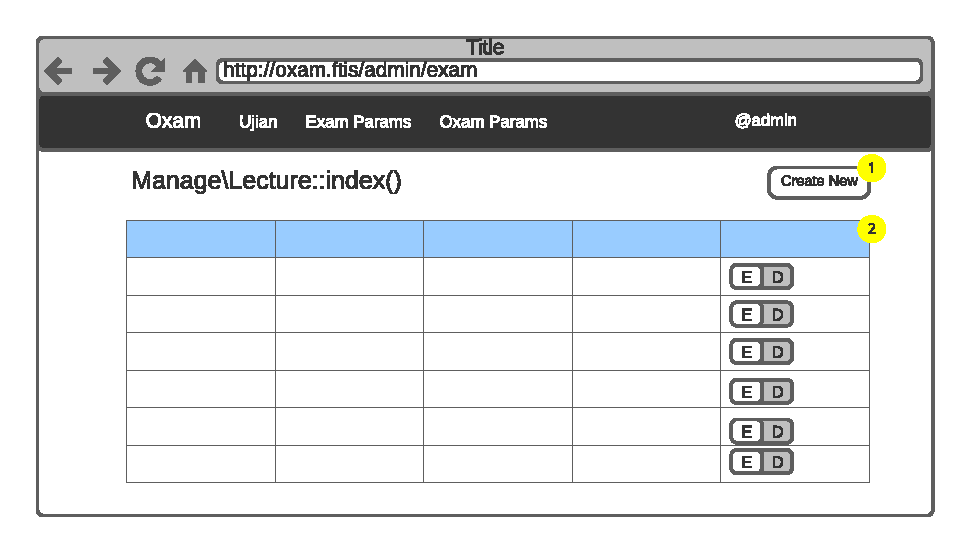
\includegraphics{Gambar/mockups/Mockup--Admin - Entity Lister.pdf}
        \caption{Rancangan antarmuka untuk daftar entri entitas.}
        \label{fig:mockup_admin_entity_lister}
    \end{figure}
    Selain ujian, tim admin dapat mengelola entri dari entitas. Rancangan
    antarmuka pertama untuk pengelola entri adalah daftar entri. Setiap entitas
    yang ada akan memiliki sebuah daftar yang disajikan dengan tabel
    terdefinisi. Rancagan antarmuka tersebut dapat dilihat pada Gambar
    \ref{fig:mockup_admin_entity_lister}.
    
    Seperti rancangan antarmuka lainnya, bagian yang ditunjukkan oleh poin-poin
    dideskripsikan sebagai berikut:
    \begin{itemize}
        \item Poin 1 adalah tombol untuk membuat entri baru. Tombol ini akan
            mengarahkan admin ke halaman \textit{editor} dengan bidang yang
            tidak terisi.
            
        \item Poin 2 adalah daftar entri yang terdapat pada entitas tersebut.
            Setiap entri akan memiliki tombol ubah dan hapus. Tombol ubah kan
            mengarahkan admin ke halaman \textit{editor} dengan bidang yang
            terisi dari entri terpilih. Tombol hapus akan memunculkan modal
            konfirmasi penghapusan entri.
            
            Daftar entri disajikan dalam bentuk tabel yang telah didefinisikan
            konfigurasinya. Tiap entri yang dapat dikelola akan memiliki sebuah
            daftar definisi yang ditentukan oleh pengembang. Berkas definisi
            tersebut akan dapat menentukan aturan kolom-kolom tertentu yang
            ingin ditampilkan.
    \end{itemize}
    
\subsubsection{Pengelola Entitas: Buat dan Ubah Entri Baru}
    \begin{figure}
        \centering
        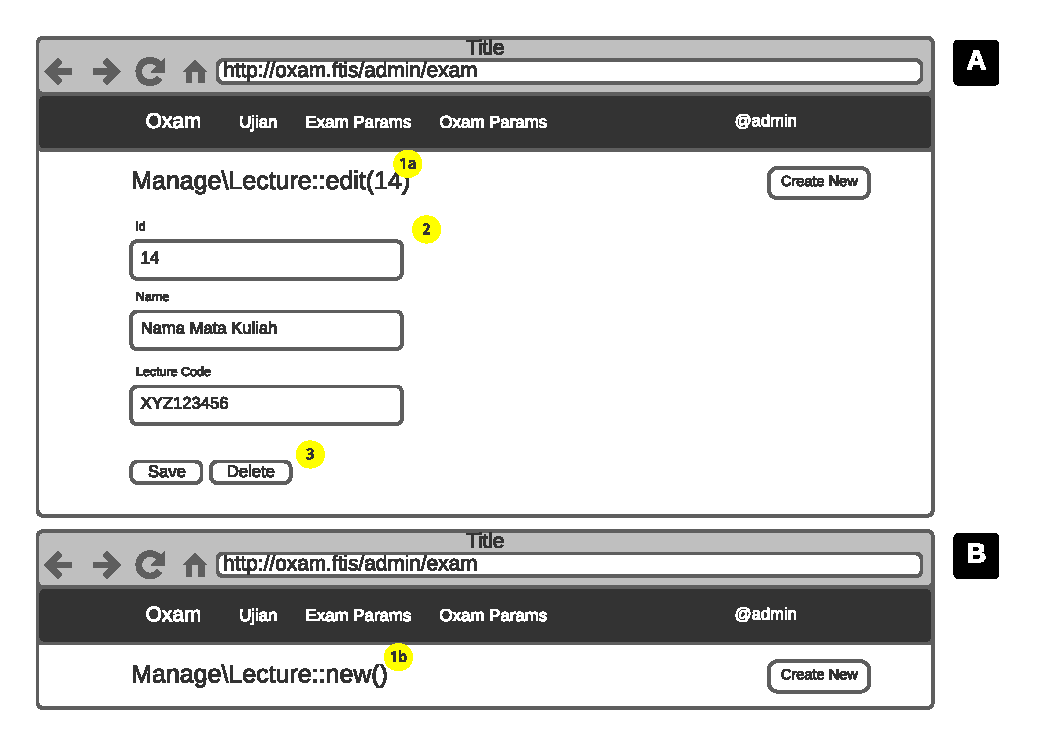
\includegraphics[width=0.75\paperwidth]{Gambar/mockups/Mockup--Admin - Entity Editor.pdf}
        \caption{Rancangan antarmuka untuk \textit{editor} entri.\\ (A) Buat
        baru; (B) Ubah yang sudah ada.}
        \label{fig:mockup_admin_entity_editor}
    \end{figure}
    Entri dari entitas dapat diubah dengan bantuan \textit{editor}. Rancangan
    tampilan \textit{editor} tersebut dapat dilihat pada Gambar
    \ref{fig:mockup_admin_entity_editor}. Secara garis besar, tampilan ini akan
    memiliki tanggung jawab untuk membuat dan mengubah data entri baru maupun
    yang sudah ada. Bagian-bagian yang ditunjukan dengan poin dideskripsikan
    sebagai berikut
    \begin{itemize}
        \item Poin 1a judul menunjukkan informasi status bahwa \textit{editor}
            akan melakukan perubahan pada entitas dengan id 14. Jika status
            editor adalah untuk membuat entri baru, maka judul akan tampil mirip
            seperti poin 1b.
        
        \item Poin 2 adalah daftar atribut yang dapat diubah atau isi nilainya,
        berdasarkan berkas definisi tabel.
        
        \item Poin 3 adalah tombol aksi untuk melakukan penyimpanan atau
            penghapusan pada entri yang saat ini dibuka. Tombol simpan akan
            mengarahkan kembali admin ke halaman daftar entri setelah perubahan
            disimpan atau entri dibuat. Tombol Hapus akan memunculkan modal
            konfirmasi hapus entri.
    \end{itemize}
    
    
\subsubsection{Pengelola Entitas: Hapus Entri}
    \begin{figure}
        \centering
        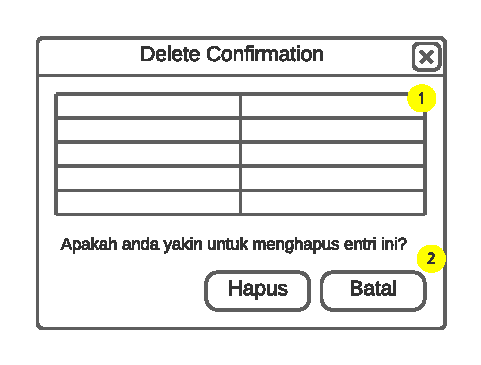
\includegraphics{Gambar/mockups/Mockup--Admin - Entity Delete.pdf}
        \caption{Rancangan antarmuka untuk menghapus entri.}
        \label{fig:mockup_admin_entity_delete}
    \end{figure}
    Pada saat tombol hapus pada halaman daftar entri dan \textit{editor} entri
    diklik, sebuah modal konfirmasi penghapusan akan dimunculkan oleh sistem.
    Rancangan modal tersebut dapat dilihat pada
    \ref{fig:mockup_admin_entity_delete}. Secara garis besar, informasi yang
    dimunculkan pada modal (poin 1) adalah kolom yang ditampilkan pada halaman
    \textit{editor}. Informasi tersebut ditampilkan untuk menyakinkan admin
    bahwa admin akan menghapus entri yang tepat.
    
    Jika modal muncul pada halaman \textit{editor}, maka setelah aksi
    penghapusan berhasil dilakukan, admin akan diarahkan menuju halaman daftar
    entri. Namun jika modal muncul pada halaman entri, admin tidak akan
    diarahkan kemanapun.
    
\subsection{Rancangan Antarmuka untuk Dosen Pengawas}
    % Jelasin kalo ini buat di proyektor
    Antarmuka untuk dosen pengawas akan bertanggung jawab untuk membuka dan
    menutup lembar jawab, serta menampilkan informasi ujian di proyektor tiap
    ruangan. Tampilan yang ada akan memiliki daftar ujian yang berbeda tiap
    ruangan, tergantung dari ujian yang diaktifkan pada ruangan tersebut.
    Untuk dapat mengkases antarmuka ini, Dosen Pengawas diharuskan untuk
    melakukan otentikasi terlebih dahulu.
    
\subsubsection{Otentikasi}
    % Screen login by IP
    \begin{figure}
        \centering
        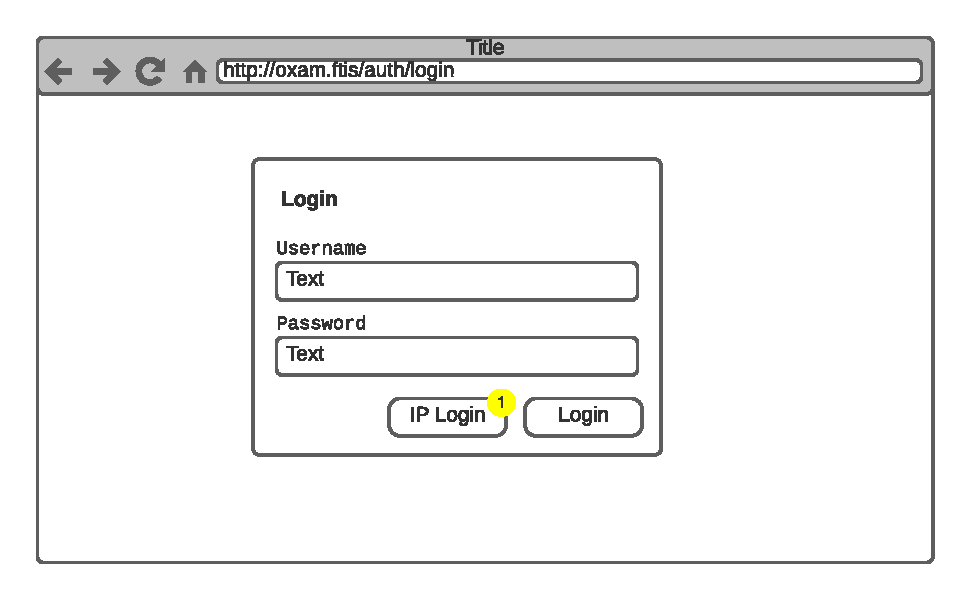
\includegraphics[width=0.7\paperwidth]{Gambar/mockups/Mockup--DosenPengawas - Login.pdf}
        \caption{Rancangan antarmuka untuk otentikasi, dengan menekankan bagian tertentu.}
        \label{fig:mockup_dosen_login}
    \end{figure}
    Tahap pertama untuk dapat mengakses layar timer, pengguna harus melakukan
    login terlebih dahulu. Serupa dengan halaman Login yang digunakan untuk
    otentikasi Admin pada Gambar \ref{fig:mockup_admin_login}, otentikasi untuk
    pengguna jenis ini dipertegas dengan penggunaan tombol IP Login yang
    ditunjukan pada poin 1 di Gambar \ref{fig:mockup_dosen_login}.
    
    Tombol IP Login pada Gambar \ref{fig:mockup_dosen_login} akan langsung
    mengarahkan pengguna ke halaman peta ruangan ujian dan timer ujian. IP dari
    komputer yang digunakan untuk mengakses halaman ini harus diregistrasikan ke
    sistem untuk proses otentikasi dapat berhasil. Jika otentikasi gagal,
    halaman ini harus menampilkan pesan kesalahan yang mendeskripsikan bahwa IP
    komputer tidak teregistrasi.
    
    % Screen Seatmap
\subsubsection{Peta Ruangan}
    \begin{figure}
        \centering
        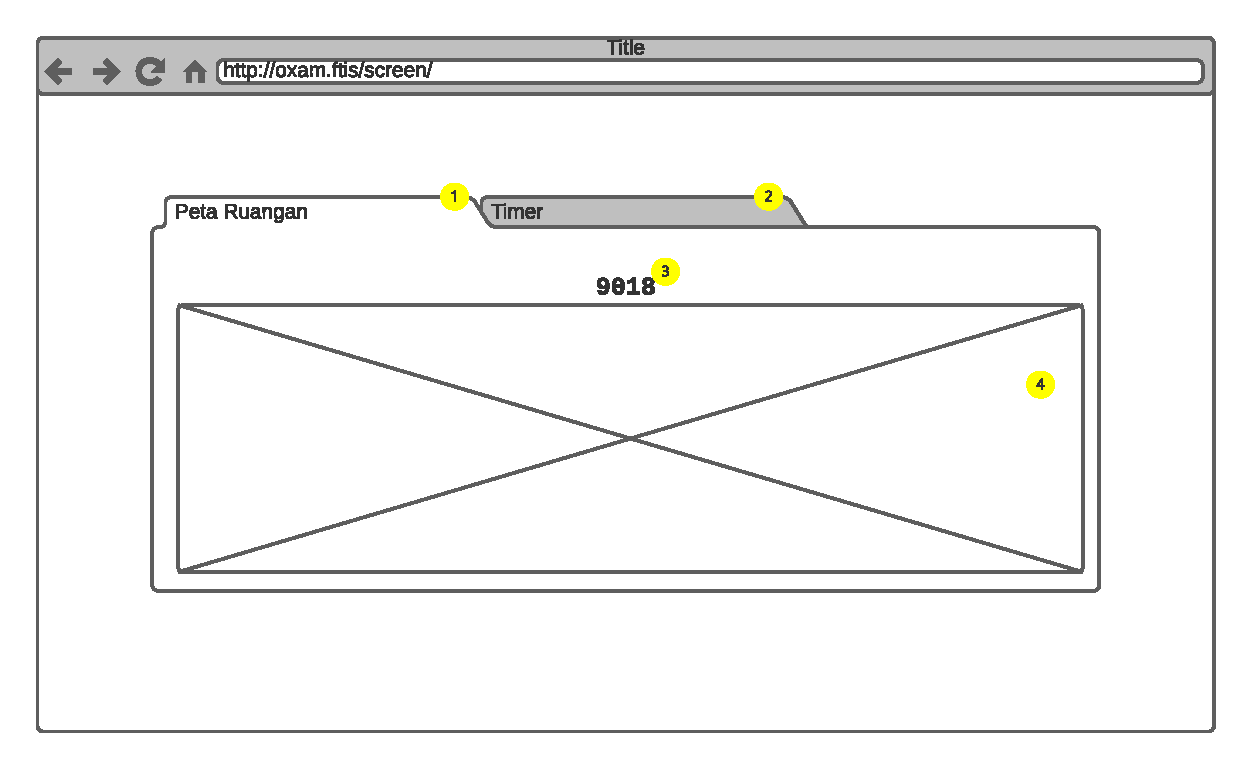
\includegraphics[width=0.7\paperwidth]{Gambar/mockups/Mockup--DosenPengawas - Seatmap.pdf}
        \caption{Rancangan antarmuka untuk halaman Peta Ruangan Ujian.}
        \label{fig:mockup_dosen_seatmap}
    \end{figure}
    Setelah otentikasi berhasil, dosen pengawas akan diarahkan menuju halaman
    peta tempat duduk ruangan ujian. Rancangan halaman informasi peta ruangan
    dapat dilihat pada Gambar \ref{fig:mockup_dosen_seatmap}. Pada halaman ini,
    informasi tentang nomor ruangan dan peta tempat duduk ruangan tersebut akan
    ditampilkan secara diagram.
    
    Bagian-bagian yang ditunjukkan oleh poin pada Gambar
    \ref{fig:mockup_dosen_seatmap} dijelaskan sebagai berikut
    \begin{itemize}
        \item Bagian yang ditunjukan oleh poin 1 dan poin 2 pada Gambar
            \ref{fig:mockup_dosen_seatmap} adalah nagivasi untuk menuju halaman
            timer dan peta ruangan. Navigasi ditambahkan untuk memudahkan dosen
            untuk melihat ujian yang akan berjalan dan peta ruangan yang ada
            saat ini. Saat pengguna pindah ke \textit{tab} lain, halaman tidak
            akan disegarkan atau mengalami pemuatan ulang. 
            
        \item Poin 3 dan 4 masing-masing menunjukkan informasi nama ruangan, dan
            peta tempat duduk dari ruangan tersebut. Poin 3 akan menunjukan nama
            ruangan yang ada dan poin 4 menunjukkan peta ruangan ujian. Peta ini
            dirancang untuk membantu peserta untuk mencari tempat duduk mereka.
            Sistem akan menampilkan tempat duduk tempat komputer yang terdaftar
            pada sistem. Informasi tentang posisi komputer akan disimpan
            pada database.
    \end{itemize}
    % Screen Timer
\subsubsection{Timer Ujian}
    \begin{figure}
        \centering
        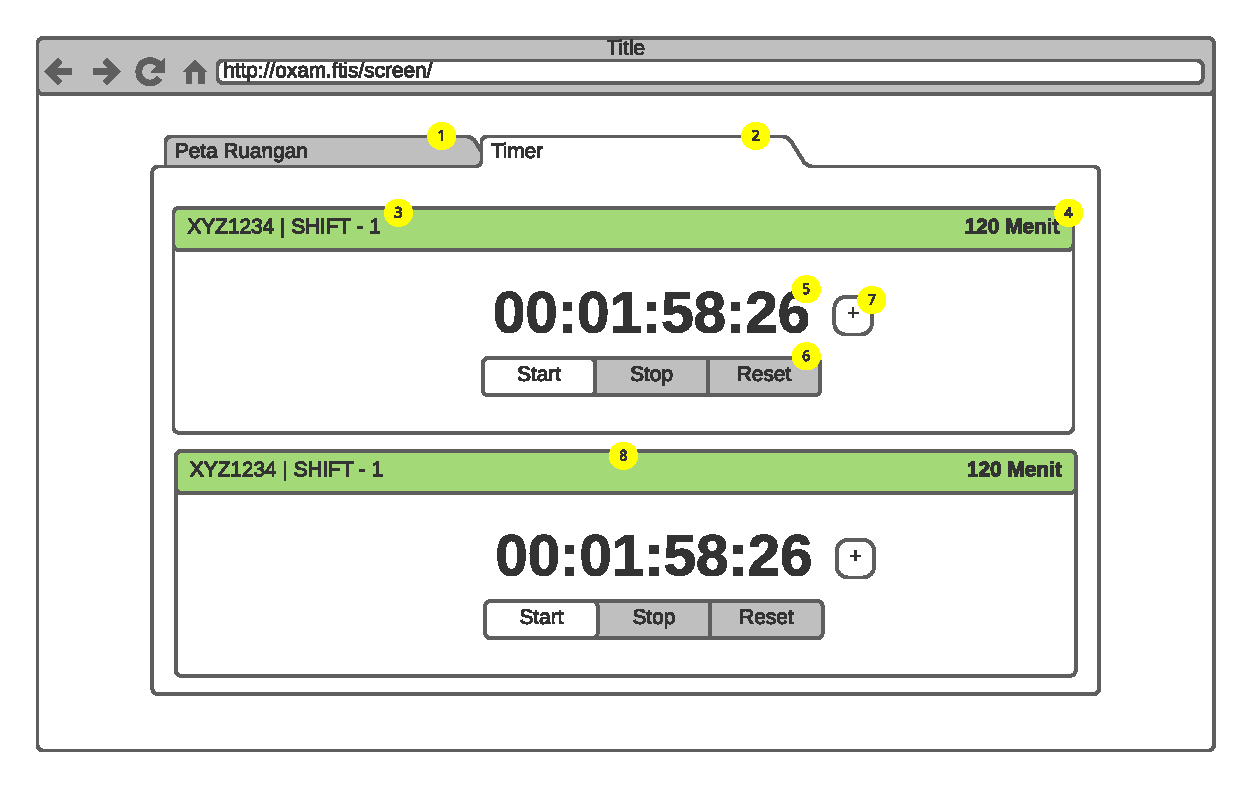
\includegraphics[width=0.75\paperwidth]{Gambar/mockups/Mockup--DosenPengawas - Timer.pdf}
        \caption{Rancangan antarmuka untuk halaman Timer.}
        \label{fig:mockup_dosen_timer}
    \end{figure}
    
    \begin{figure}
        \centering
        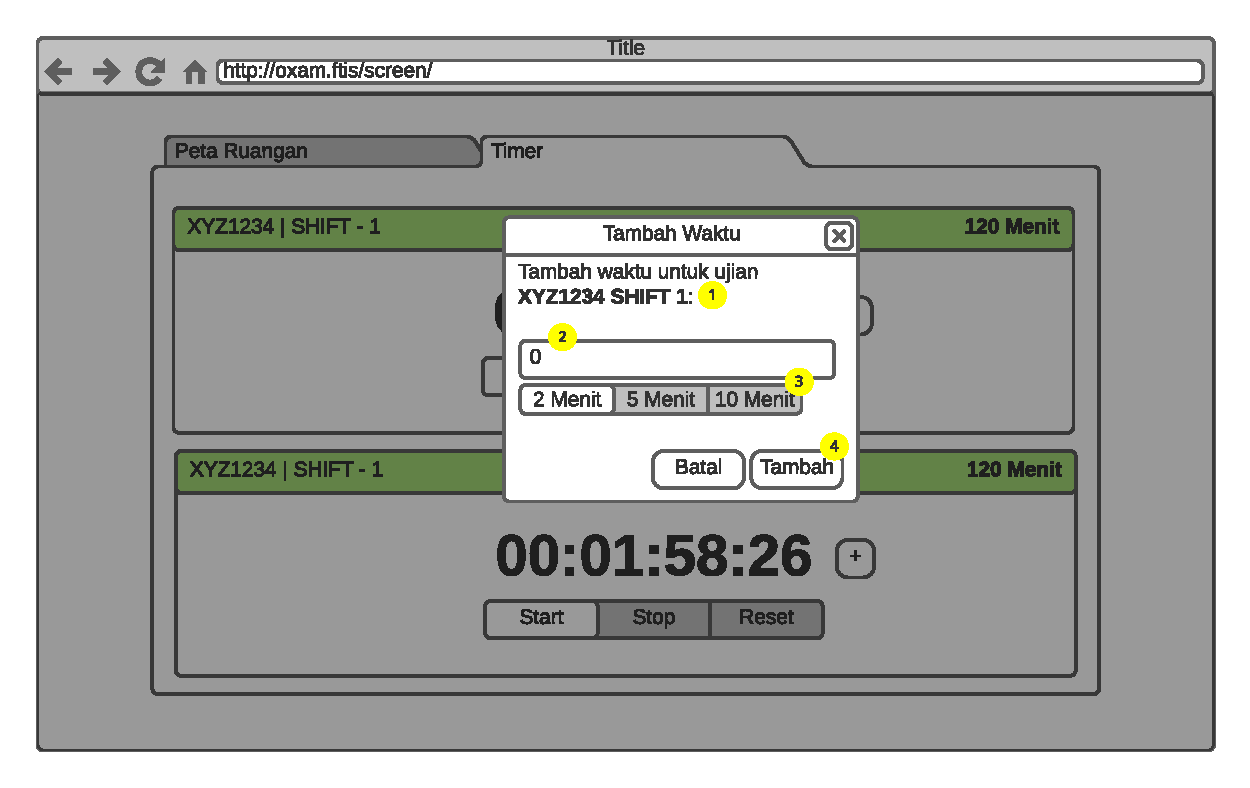
\includegraphics[width=0.75\paperwidth]{Gambar/mockups/Mockup--DosenPengawas - Timer + Overtime.pdf}
        \caption{Rancangan antarmuka untuk \textit{Overtime} Ujian.}
        \label{fig:mockup_dosen_overtime}
    \end{figure}
    
    Rancangan halaman timer ujian dapat diperhatikan pada Gambar
    \ref{fig:mockup_dosen_timer}. Secara keseluruhan, halaman timer akan
    menampilkan informasi ujian singkat, waktu tersisa dan tombol-tombol alat
    untuk memanipulasi waktu ujian.
    
    Mengikuti rancangan antarmuka Peta Ruangan, halaman timer memiliki bagian
    navigasi seperti yang ditunjukan pada poin 1 dan 2 pada Gambar
    \ref{fig:mockup_dosen_timer}. Karena saat ini pengguna sedang membuka
    \textit{tab} Timer, maka kepala \textit{tab} yang aktif menunjukkan kepala
    \textit{tab} timer. Dosen pengawas dapat melihat kedua informasi tersebut
    dengan mudah. Bagian pada rancangan tampilan tersebut dideskripsikan sebagai
    berikut:
    
    \begin{itemize}
       % poin 3
        \item Bagian yang ditunjukkan pada poin 3 adalah informasi ujian secara
            singkat. Informasi yang ditunjukkan berupa kode mata kuliah dan
            \textit{shift}nya. Informasi ini nantinya dapat digunakan untuk
            membedakan ujian satu dengan yang lainnya pada tampilan multiujian.
            
        % poin 4
        \item Bagian yang ditunjukkan pada poin 4 adalah jumlah durasi waktu
            yang diberikan untuk ujian ini. Durasi lamanya ujian ini akan
            diambil dari basis data dan tidak akan berkurang mengikuti tampilan
            timer.
        
        % poin 5
        \item Bagian yang ditunjukan oleh poin 5 adalah tampilan timer. Timer
            ini akan memiliki nilai dasar total durasi dari ujian. Timer akan
            mulai berjalan saat kontrol yang ditunjukan pada poin 6 mulai
            digunakkan. Pada saat timer mencapai nilai nol, maka tampilan
            tersebut akan dipertahankan selama beberapa menit untuk memastikan
            dosen pengawas dapat menambahkan waktu lebih sebelum lembar jawab
            tidak dapat diubah kembali.
        
        % poin 6
        \item Poin 6 menunjukkan bagian kontrol dari timer ujian. Kontrol
            akan terdiri dari tombol aksi mulai berhenti, dan setel ulang.
            Tombol-tombol ini akan langusng melakukan panggilan API
            ke sistem back-end.
        
        % poin 7
        \item Poin 7 menunjukkan tombol tambahan \textit{overtime}. Tombol ini
            digunakan untuk menambahkan waktu ujian jika sewaktu-waktu
            dibutuhkan. Tombol akan menampilkan sebuah \textit{modal} yang
            menyediakan sebuah formulir sederhana, menanyakan berapa banyak
            waktu yang ingin ditambahkan. Modal tersebut dapat dilihat pada
            Gambar \ref{fig:mockup_dosen_overtime}. Modal akan menampilan
            informasi singkat ujian (poin 9), banyak waktu yang diinginkan (poin
            10), tombol cepat untuk menambahkan waktu (poin 11), dan tombol
            \textit{submit} dan batalkan (poin 12).
        
        % poin 8
        \item Poin 8 adalah contoh timer lain yang ditunjukkan jika terdapat
            ujian lain yang akan diadakan pada ruangan yang sama. Tampilan akan
            memiliki bentuk tataletak yang sama, sehingga yang menjadi pembeda
            hanyalah bagian kepala (ditunjukkan pada poin 3).
    \end{itemize}
    
    
\subsection{Rancangan Antarmuka Tambahan}
    Rancangan antarmuka tambahan ini muncul dari kebutuhan untuk sistem
    mengirimkan laporan ujian dengan tambahan halaman pengunduhan. Oleh karena
    itu, pada bagian ini akan dibahas rancangan antarmuka untuk email dan
    halaman pengunduhannya.
    
    % Email
\subsubsection{Email Laporan}
    \begin{figure}
        \centering
        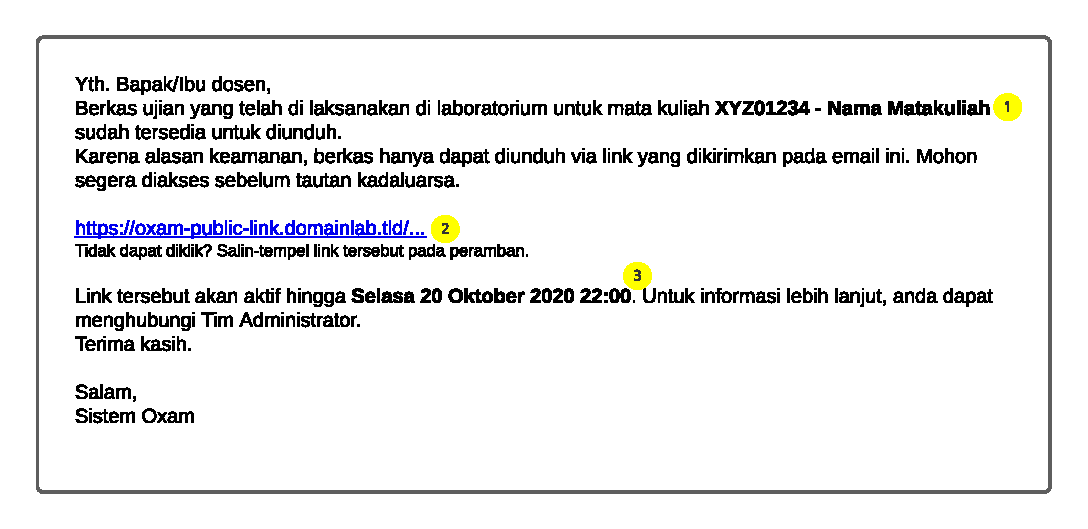
\includegraphics[width=0.7\paperwidth]{Gambar/mockups/Mockup--Tambahan.pdf}
        \caption{Rancangan antarmuka untuk email laporan ujian.}
        \label{fig:mockup_addition_email}
    \end{figure}
    Email yang akan dikirimkan sebagai laporan akan dibuat dengan teknologi
    HTML, seperti pada umumnya. Email akan berisi sebuah tautan menuju halaman
    untuk mengunduh berkas jawaban ujian. Email juga akan berisi beberapa
    informasi krusial tentang masa hidup tautan tersebut sehingga penerima
    laporan tidak merasa kebingungan jika tautan tidak dapat diakses.
    
    Rancangan untuk tampilan email dapat dilihat pada Gambar
    \ref{fig:mockup_addition_email}. Seperti yang ditunjukkan pada gambar, email
    akan memiliki sejumlah instruksi untuk mengunduh berkas jawaban, informasi
    mata kuliah ujian (Poin 1 dari Gambar \ref{fig:mockup_addition_email}),
    tautan untuk mengunduh berkas jawaban tersebut (Poin 2 dari Gambar
    \ref{fig:mockup_addition_email}), dan informasi kapan tautan tersebut akan
    kadaluarsa (Poin 3 dari Gambar \ref{fig:mockup_addition_email}).
    
    % Autonomus download
\subsubsection{Halaman Pengunduhan Berkas Jawaban Ujian}
    Tautan yang dikirim lewat email akan mengarah pada halaman ini. Informasi
    singkat tentang ujian akan ditampilkan pada halaman ini sebelum akhirnya
    penerima laporan dapat melakukan pengunduhan hasil jawaban tersebut. Halaman
    ini dirancang untuk disediakan oleh sistem Oxam yang dapat diakses via
    internet.
    
    \begin{figure}
        \centering
        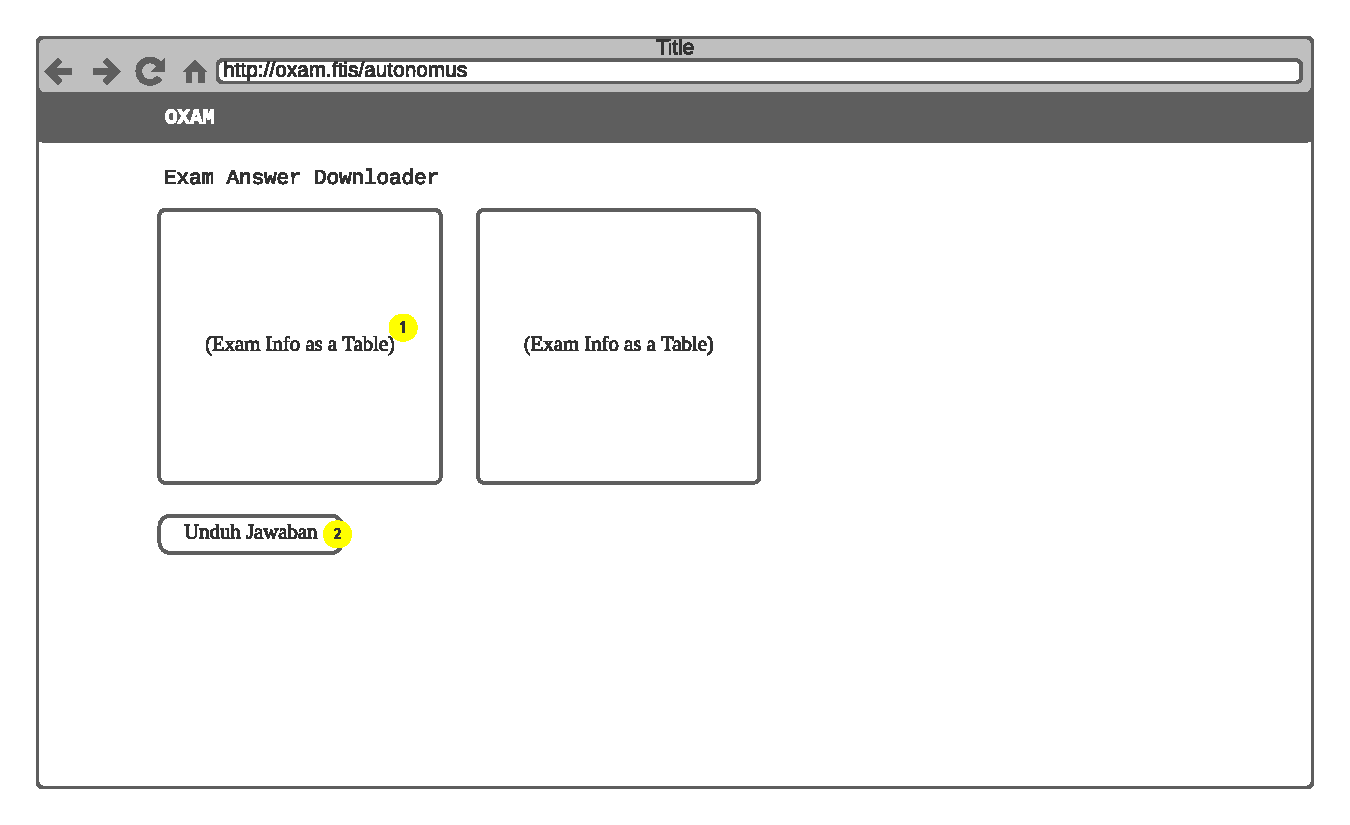
\includegraphics[width=0.7\paperwidth]{Gambar/mockups/Mockup--Tambahan - Exam-extractor.pdf}
        \caption{Rancangan antarmuka untuk halaman pengunduhan berkas jawaban ujian.}
        \label{fig:mockup_addition_downloader}
    \end{figure}
    Rancangan halaman pengunduhan dapat dilihat pada Gambar
    \ref{fig:mockup_addition_downloader}. Bagian yang ditunjukkan oleh Poin 1
    pada Gambar \ref{fig:mockup_addition_downloader} adalah informasi ujian yang
    disajikan dalam bentuk tabel. Tabel ini nantinya akan berisi semua informasi
    dari entitas ujian, dengan penyesuaian tertentu. Lalu bagian yang
    ditunjukkan pada poin 2 adalah tombol unduh jawaban ujian. Tombol ini akan
    memaksa peramban untuk melakukan pengunduhan berkas jawaban ke komputer
    penerima laporan.
    
\section{Perancangan Sistem Backend}
    Sesuai dengan perannya, sistem backend akan bertanggung jawab menangani
    bagian-bagian yang hanya ditangani pada sisi server. Tanggung jawab
    tersebut mulai dari melakukan pengolahan data, pengelolaan basis data, serta
    menyediakan API yang digunakan oleh sistem frontend untuk berkomunikasi.
    
    Pada bagian ini akan dijelaskan perancangan sistem untuk subsistem backend.
    Penjelasan tersebut dimulai dari pembahasan perancangan basis data,
    perancangan REST API serta desain kelas dari subsistem ini.
    
\subsection{Racangan Basis Data}
    \begin{sidewaysfigure}
        \centering
        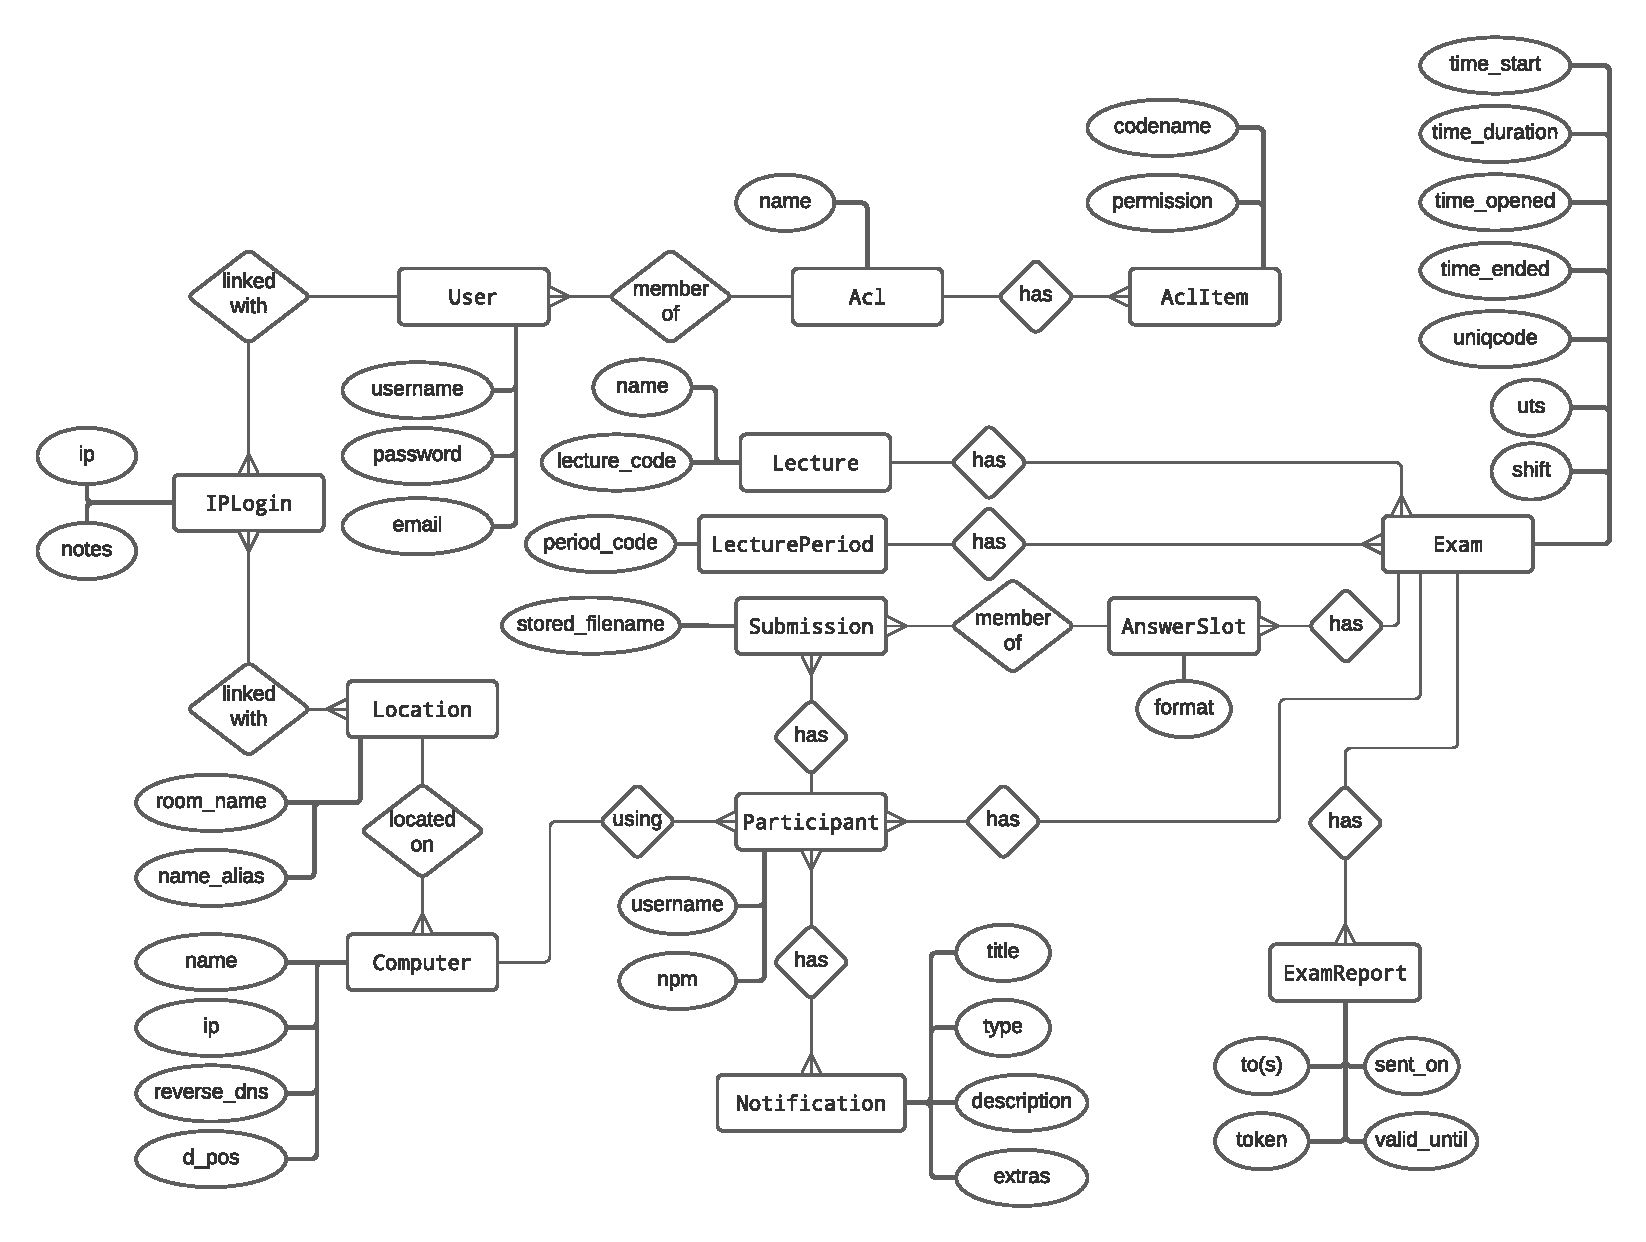
\includegraphics[width=1\paperwidth]{Gambar/erd-rev-b.pdf}
        \caption{Diagram \textit{ERD} untuk sistem aplikasi yang baru.}
        \label{fig:erd_overview}
    \end{sidewaysfigure}
    
    Perancangan basis data dimulai dengan merumuskan entitas yang dibutuhkan dan
    relasinya dengan entitas lainnya. Rumusan tersebut direpresentasikan dalam
    bentuk diagram relasi entitas atau ERD. Diagram ERD untuk aplikasi ini dapat
    dilihat pada Gambar \ref{fig:erd_overview}. Berdasarkan kebutuhan yang
    dianalisis pada bab sebelumnya, sistem membutuhkan empat belas entitas yang
    bertanggung jawab untuk merepresentasikan struktur data yang digunakan.
    Setiap entitas yang dibuat akan dibuat ulang representasinya dalam bentuk
    kelas pada sistem PHP dengan harapan membantu penanganan dan perancangan
    sistem REST API.
    
    Pembahasan akan dilanjutkan dengan menjelaskan satu per satu entitas yang
    ditunjukan pada diagram ERD. Pembahasan akan dimulai dengan entitas yang
    penulis kategorikan sebagai esensial untuk sistem terlebih dahulu, lalu
    dilanjutkan dengan entitas yang muncul dari analisis dari bab sebelumnya.
    
\subsubsection{User}
    % TODO: Figure mini user?.
    Entitas \texttt{User} merepresentasikan pengguna aplikasi. Entitas ini akan
    menyimpan informasi khusus seperti nama pengguna (\texttt{username}), kata
    sandi (\texttt{password}) dan email. Kolom \texttt{password} pada entitas
    ini akan di\textit{hash} menggunakan algoritma Blowfish dengan bantuan
    \textit{library} dari PHP dengan alasan keamanan.
    
    Entitas ini dinilai esensial karena entitas ini digunakan untuk melakukan
    otentikasi menuju panel admin. Entitas ini akan memiliki perlakuan khusus
    pada saat data dari entitas ini ditransmisikan ke sistem frontend.
    Otentikasi ini penting untuk mengkhususkan peran dari setiap pengguna.

\subsubsection{ACL dan ACLItem}
    \begin{figure}[H]
        \centering
        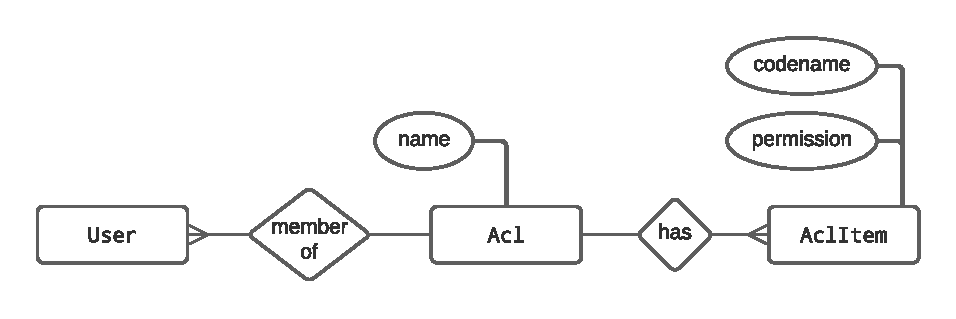
\includegraphics[width=0.75\paperwidth]{Gambar/erd-details/ERD--New - ACL & ACLItem.pdf}
        \caption{Potongan diagram entitas untuk \texttt{ACL} dan
        \texttt{ACLItem}.}
        \label{fig:erd_acl-aclitem}
    \end{figure}
    
    Entitas \texttt{ACL} dan \texttt{ACLItem} adalah entitas yang menampung
    informasi tentang peran dan izin untuk setiap pengguna, diperjelas pada
    Gambar \ref{fig:erd_acl-aclitem}. \texttt{ACL} menyimpan grup utama dari
    \texttt{ACLItem}, atau dapat kita sebut sebagai peran. Sedangkan
    \texttt{ACLItem} menyimpan informasi izin untuk setiap nama kasus
    (\texttt{codename}) yang diperbolehkan.
    
    \begin{table}[H]
        \centering
        \begin{tabular}{|l|l|l|}
        \hline
        Label & Deskripsi & Nilai Biner \\ \hline
        C     & Buat      & \texttt{0b0001}        \\ \hline
        R     & Baca      & \texttt{0b0010}        \\ \hline
        U     & Perbarui  & \texttt{0b0100}        \\ \hline
        D     & Hapus     & \texttt{0b1000}        \\ \hline
        \end{tabular}
        \caption{Tabel representasi nilai biner pada kolom \texttt{permission}
        di entitas \texttt{ACLItem}.}
        \label{tab:aclitem_level}
    \end{table}
        
    
    Perizinan direpresentasikan dengan menggunakan sistem biner yang disimpan
    pada database sebagai angka. Representasi biner ini terdiri dari label CRUD,
    dengan C adalah Buat (\textit{Create}), R adalah Baca (\textit{Read}), U
    adalah Perbaharui (\textit{Update}) dan D adalah Hapus (\textit{Delete}).
    Label tersebut kemudian diberikan tempat khusus pada bitstring sebelum
    akhirnya dikonversi sebagai angka. Nilai-nilai tersebut dapat dilihat pada
    tabel \ref{tab:aclitem_level}.
    
    
    Sebagai contoh, seorang pengguna dapat \textbf{membuat}, \textbf{membaca},
    \textbf{memperbarui} namun tidak dapat menghapus sebuah entri. Nilai dari
    tabel \ref{tab:aclitem_level} digabungkan dengan operator \texttt{OR} untuk
    setiap izin yang diberikan. Dengan demikian, nilai \texttt{permission} yang
    diberikan adalah sebagai berikut:
    
    \begin{subequations}
        \begin{align}
            C \vee R \vee U \vee 0b0000 &= K\\
            0b0001 \vee 0b0010 \vee 0b0100 \vee 0b0000 &= K \\
            K &= 0b0111 \\
            K &= 7
        \end{align}
    \end{subequations}
    
    Hasil kalkulasi kode izin tersebut akan disimpan sebagai 7 pada database
    sebagai representasi kode izin \texttt{0b000}. 
    
    Pengecekan izin \texttt{permission} dilakukan dengan memanfaatkan operator
    \texttt{AND} antara nilai pada kolom \texttt{permission} dengan nilai
    \texttt{permission} yang diekspektasikan, lalu dibandingkan dengan nilai
    ekspektasi. Sebagai contoh, sistem perlu mengecek apakah pengguna dapat
    membuat sebuah entri. Sistem dapat melakukan pengecekkan dengan melakukan
    operasi \texttt{AND} pada nilai \texttt{permission} yang ada saat ini
    (\texttt{0111}) dengan nilai \texttt{permission} yang diekspektasi
    (\texttt{0010}), dan hasilnya dibandingkan dengan hasil ekspektasi.
    Kalkulasi yang dilakukan dapat dilihat pada simulasi ekuasi berikut:
    
    \begin{subequations}
        \begin{align}
            K \wedge C &= C \\
            0b0111 \wedge C &= C \\
            0b0111 \wedge 0b0001 &= 0b0001 \\
            0b0001 &= 0b0001 \\
            \text{True}
        \end{align}
    \end{subequations}
    
    Sedangkan jika pengecekan apakah seorang pengguna dapat melakukan
    penghapusan terhadap sebuah entri, perhitungan perizinannya menjadi:
    
    \begin{subequations}
        \begin{align}
            K \wedge D &= D \\
            0b0111 \wedge D &= D \\
            0b0111 \wedge 0b1000 &= 0b1000 \\
            0b0000 &= 0b1000 \\
            \text{False}
        \end{align}
    \end{subequations}
    
    Hasil dari ekuasi tersebut kemudian dapat digunakan untuk menentukan apakah
    seorang pengguna dapat melakukan aksi yang diminta atau tidak.
    
    Operasi ini terinspirasi dari \texttt{chmod} dari Linux\footnote{Lihat
    https://linux.die.net/man/1/chmod}. \texttt{chmod} menerima input berupa
    tiga angka yang merepresentasikan level akses pada \textit{resource}
    tertentu pada sistem. Tiga angka tersebut kemudian diubah menjadi biner
    untuk dilihat apakah seorang pengguna dapat melakukan aksi tertentu.
    Pendekatan ini kemudian diadaptasi pada sistem ini dengan menggunakan level
    akses yang berbeda (CRUD, dibanding RWX). Dengan demikian pengaturan dan
    pengelolaan resources pada entitas dapat lebih terkontrol dengan lebih
    fleksibel.
    
\subsubsection{IPLogin}
    \begin{figure}
        \centering
        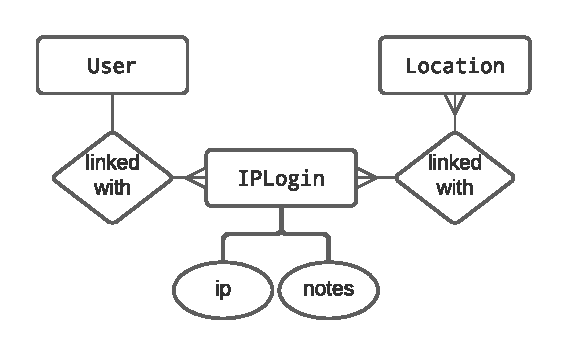
\includegraphics{Gambar/erd-details/ERD--New - IPLogin.pdf}
        \caption{Potongan diagram entitas untuk \texttt{IPLogin}.}
        \label{fig:erd_iplogin}
    \end{figure}
    Entitas \texttt{IPLogin} digunakan untuk melakukan otentikasi semi-otomatis
    dengan memanfaatkan IP pengguna pada lab, ditautkan dengan sebuah akun
    pengguna dengan peran yang terbatas (hanya dapat melihat dan mengubah
    entitas tertentu), diperjelas pada Gambar \ref{fig:erd_iplogin}. Entitas
    menyimpan informasi IP, tautan pada pengguna dan lokasi-lokasi, serta
    catatan khusus tentang penautan tersebut. 
    
    Entitas ini memiliki hubungan \textit{many-to-many} dengan entitas
    \texttt{Location}. Relasi ini diharapkan agar Tim Admin dapat melakukan
    pengaturan komputer master untuk melihat seluruh ujian yang aktif pada
    ruangan tertentu tanpa harus membuatkan akun khusus tertentu pada sistem.
    Tim Admin dapat dengan mudah menautkan sejumlah ruangan yang diinginkan
    dengan akun yang memiliki peranan terbatas yang sudah ada sebelumnya.
    
    Entitas ini dinilai cukup esensial karena berhubungan dengan sistem
    otentikasi yang membatasi pengguna untuk melakukan aksi tertentu di admin
    panel.
    
\subsubsection{Location dan Computer}
    \begin{figure}
        \centering
        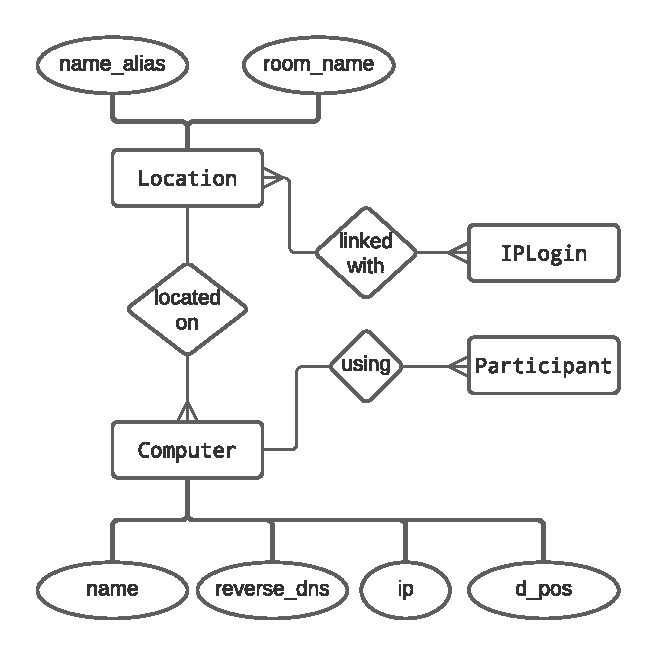
\includegraphics{Gambar/erd-details/ERD--New - Location & Computer.pdf}
        \caption{Potongan diagram entitas untuk \texttt{Location} dan
        \texttt{Computer}.}
        \label{fig:erd_location-computer}
    \end{figure}
    
    Entitas \texttt{Location} dan \texttt{Computer} menyimpan informasi tentang
    lokasi (ruagan) dan daftar pada komputer tersebut sebelum nantinya
    dihubungkan dengan entitas lainnya. Hubungan antara kedua entitas tersebut
    dapat diperhatikan pada potongan diagram entitas di gambar
    \ref{fig:erd_location-computer}.
    
    Entitas \texttt{Location} menyimpan informasi lokasi dan ruangan tempat
    peserta dapat mengikuti ujian. Pada entitas ini, informasi yang disimpan
    adalah nama ruangan tersebut dan nama lain dari ruangan tersebut.
    Berdasarkan survei lapangan, setiap ruangan memiliki nama lain, sehingga
    kolom \texttt{name\_alias} ditambahkan. Sedangkan nama ruangan disimpan pada
    kolom \texttt{room\_name}.
    
    Entitas \texttt{Computer} mendefinisikan komputer yang terdapat pada lokasi
    tersebut. Oleh karena itu hubungan yang dimiliki dengan entitas
    \texttt{Location} adalah \textit{one-to-many}. Entitas ini menyimpan
    informasi berupa nama komputer (\textit{name}), IPnya (\textit{ip}), nama
    FQDN (\textit{Fully Qualified Domain Name}) atau domain dari komputer
    tersebut (\textit{reverse\_dns}), dan detil letak posisi dari komputer
    tersebut pada peta ruangan (\textit{d\_pos}).
    
    Kolom \textit{d\_pos} digunakan untuk menyimpan informasi letak komputer
    pada peta dalam bentuk JSON. Bentuk format ini digunakan karena data ini
    digunakan hanya pada sistem frontend. Dengan kesepakatan yang diharapkan
    cukup fleksibel, maka bentuk pemosisian ini akan disimpan dalam bentuk JSON.
    
    Kolom \textit{ip} digunakan untuk menautkan sebuah komputer dengan IP,
    sehingga tabel otentikasi yang digunakan oleh peserta dapat langsung merujuk
    pada entitas ini. Setiap komputer peserta yang ingin digunakan akan
    didaftarkan pada entitas ini. Untuk saat ini, karena survei lapangan
    menunjukan bahwa versi IP yang digunakan adalah versi 4, maka fokus aplikasi
    saat ini akan menggunakan IPv4.
    
    Selain itu, terdapat kolom \textit{reverse\_dns} yang digunakan untuk
    menyimpan informasi nama domain dari komputer tersebut. Kolom ini diharapkan
    dapat membantu Tim Admin dan pengembang aplikasi berikutnya untuk melakukan
    \textit{debugging} dan kebutuhan API lainnya. Nama domain ini didapatkan
    dari LDAP yang digunakan oleh Server Windows untuk melakukan auditing objek
    mereka. Komputer yang terhubung dengan Active Directory milik Lab akan
    terdaftar pada sistem internal LDAP milik Windows Server yang nantinya akan
    diberikan domain khusus untuk komputer tersebut.

\subsubsection{Lecture dan LecturePeriod}

    \begin{figure}
        \centering
        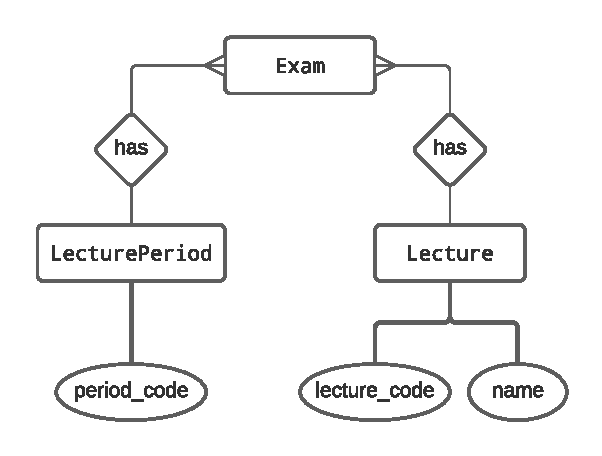
\includegraphics{Gambar/erd-details/ERD--New - Lecture & LecturePeriod.pdf}
        \caption{Potongan diagram entitas untuk \texttt{Lecture} dan
        \texttt{LecturePeriod}.}
        \label{fig:erd_lecture-lectureperiod}
    \end{figure}

    Entitas \texttt{Lecture} dan \texttt{LecturePeriod} menyimpan informasi
    tentang mata kuliah dan periode tahun ajar mata kuliah bersangkutan pada
    ujian tertentu. Hubungan antara kedua entitas tersebut terhadap entitas
    \texttt{Exam} dapat dilihat pada potongan diagram entitas di gambar
    \ref{fig:erd_lecture-lectureperiod}.  Entitas \texttt{Lecture} menyimpan
    informasi nama mata kuliah beserta kodenya, dan \texttt{LecturePeriod}
    menyimpan informasi tahun ajaran dalam bentuk kode.
    
    \begin{table}[]
        \centering
        \begin{tabular}{|l|l|}
        \hline
        Nilai & Tipe Semester \\ \hline
        1     & Ganjil        \\ \hline
        2     & Genap         \\ \hline
        3     & Pendek        \\ \hline
        \end{tabular}
        \caption{Definisi tipe semester dengan nilainya untuk kolom
            \texttt{period\_code} pada entitas \texttt{LecturePeriod}.}
        \label{tab:lecture-periode}
    \end{table}
    
    Kode tersebut terdiri dari lima digit angka yang terdiri dari tahun ajar dan
    tipe semester yang sedang berjalan. Empat digit pertama adalah tahun ajar,
    dan satu digit terakhir adalah tipe semester. Tipe semester dan nilai
    representasinya dapat dilihat lebih jelas pada tabel
    \ref{tab:lecture-periode}.
    
    Sebagai contoh, semester ganjil pada tahun ajar 2016-2017 direpresentasikan
    sebagai \texttt{20161}. Empat digit pertama diambil dari tahun ajar pada
    tahun dimulai, 2016. Lalu berdasarkan tabel \ref{tab:lecture-periode},
    semester ganjil memiliki nilai representasi 1, sehingga kode untuk tahun
    ajar yang disimpan pada kolom \textit{period\_code} adalah \texttt{20161}.
    
\subsubsection{Participant}
    \begin{figure}
        \centering
        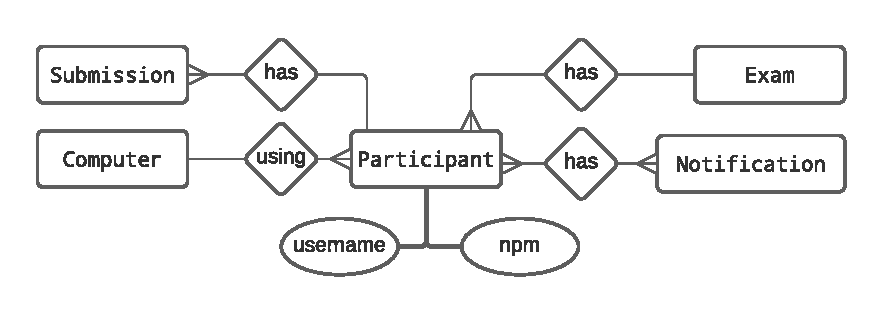
\includegraphics{Gambar/erd-details/ERD--New - Participant.pdf}
        \caption{Potongan diagram entitas untuk \texttt{Participant}.}
        \label{fig:erd_participant}
    \end{figure}
    
    Entitas \texttt{Participant} digunakan untuk menyimpan informasi tentang
    peserta ujian di lab. Seperti pada potongan diagram relasi entitas pada
    gambar \ref{fig:erd_participant}, entitas ini hanya memiliki dua kolom utama
    yang digunakan untuk merepresentasikan seorang peserta. Kolom
    \texttt{username} untuk menyimpan informasi username pada sistem dan
    \texttt{npm} untuk menyimpan informasi NPM dari peserta.
    
    Kolom \texttt{npm} digunakan untuk menyimpan string \textit{literal} dari
    nomor pokok mahasiswa (NPM). Karena NPM mahasiswa yang aktif pada saat
    penelitian ini dibuat terdapat dua standar, maka untuk memperingan kinerna
    basis data, string \textit{literal} NPM ikut disimpan.
    
    Sedangkan kolom \texttt{username} digunakan untuk menyimpan username yang
    biasa digunakan di lab untuk login. Kolom ini akan berguna untuk membantu
    sistem mebuat \textit{script batch} pada tahap pemberian akses ke berkas
    bantuan ujian dan \textit{workspace} peserta ujian. Pemberian akses dengan
    script membutuhkan nama pengguna yang digunakan untuk login.
    
\subsubsection{AnswerSlot}
    Entitas \texttt{AnswerSlot} digunakan untuk menyimpan informasi tentang slot
    jawaban pada ujian tertentu. Entitas ini digunakan sebagai panduan untuk
    sistem memberikan informasi tentang format penamaan file, disimpan pada
    kolom \texttt{format}. Seperti yang terlihat pada diagram entitas pada
    \ref{fig:erd_overview}, entitas ini akan terhubung secara
    \textit{many-to-one} terhadap entitas \texttt{exam} dan \textit{one to many}
    pada entitas \texttt{Submission}.
    
    Jawaban yang dikirimkan oleh peserta nantinya akan disimpan pada entitas
    \texttt{Submission} dengan bantuan referensi format dari
    \texttt{AnswerSlot}. Setiap jawaban yang dikumpulkan akan dicek formatnya
    berdasarkan format yang diberikan pada entitas \textit{AnswerSlot}.

\subsubsection{ExamReport}
    Entitas \texttt{ExamReport} digunakan untuk membantu sistem menjadwalkan
    pengiriman laporan ujian. Laporan ini nantinya akan dikirimkan via email
    untuk mengatisipasi email diblokir oleh penyedia layanan email karena kode
    Java dan berkas \texttt{.class} dianggap sebagai virus.
    
    Seperti yang ditunjukkan pada diagram entitas pada gambar
    \ref{fig:erd_overview}, entitas \texttt{ExamReport} menyimpan beberapa kolom
    yang digunakan untuk membantu penjadwalan. Kolom pertama adalah
    \texttt{sent\_on} yang digunakan untuk menandakan apakah ujian ini telah
    dikirimkan pada email (\texttt{to(s)}) ini. Kolom \texttt{valid\_until}
    digunakan untuk menyimpan informasi kapan \texttt{token} akan kadaluarsa
    (\textit{expired}).
    
    Penggunaan token pada kasus ini dengan harapan alamat link yang dikirim oleh
    sistem ke dosen dapat dengan aman di akses. Kode token akan terdiri dari 16
    byte acak yang dikonversi menjadi 32 digit heksadesimal string. Token ini
    diharapkan dibangkitkan dengan standar pengacakan untuk kriptografi.
    Pengacakan dengan standar tersebut diharapkan dapat memperkecil faktor
    kemungkinan serangan prediksi kode token (\textit{guessing attack}).

\subsubsection{Exam}
    \begin{figure}
        \centering
        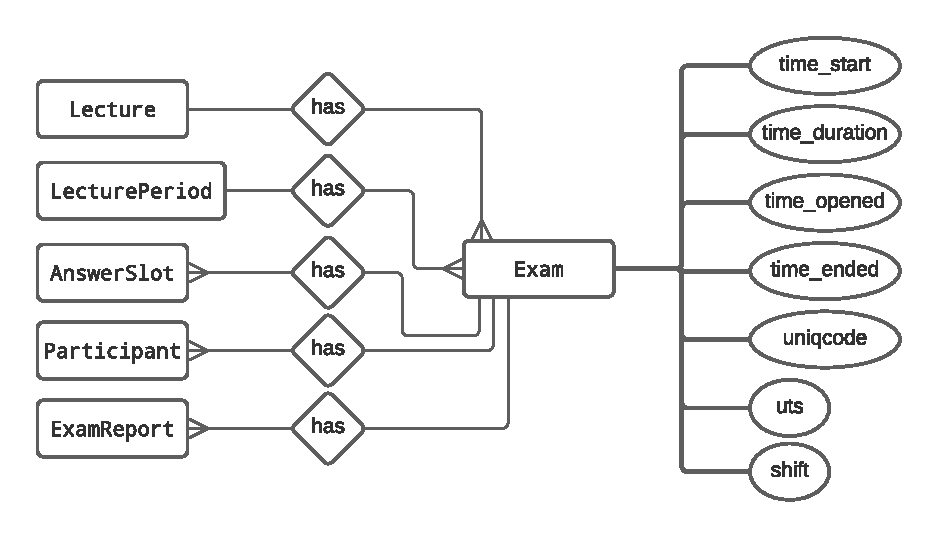
\includegraphics[width=0.75\paperwidth]{Gambar/erd-details/ERD--New - Exam.pdf}
        \caption{Potongan diagram entitas untuk \texttt{Exam}.}
        \label{fig:erd_exam}
    \end{figure}
    Entitas berikutnya yang akan dibahas adalah entitas \texttt{Exam}, dapat
    dilihat pada potongan gambar \ref{fig:erd_exam}. Entitas ini menyimpan
    informasi utama untuk ujian dan jadwalnya. Informasi jadwal disimpan pada
    kolom dengan \textit{prefix} \texttt{time\_}. Informasi dasar dari ujian
    tersebut disimpan dengan relasi langsung ke tabel lain seperti
    \texttt{Lecture}, \texttt{LecturePeriod}, \texttt{AnswerSlot}, dan
    seterusnya. 
    
    Informasi yang cukup penting pada entitas ini terdapat pada kolom
    \texttt{uniqcode}. Kolom ini menyimpan informasi kode unik dari sebuah ujian
    yang kita gunakan untuk menyimpan informasi nama folder berkas ujian. Kode
    ini diharapkan terdiri dengan byte acak yang dibangkitkan dengan standar
    pengacakan untuk kriptografi. Pengacakan dengan standar tersebut diharapkan
    dapat memperkecil faktor kemungkinan serangan prediksi kode unik
    (\textit{guessing attack}).
    
    Pengecekan ujian yang aktif dilakukan dengan melakukan pengecekan pada kolom
    \texttt{time\_start} dan \texttt{time\_ended}. Kolom \texttt{time\_start}
    menandakan informasi tentang kapan ujian \textbf{akan} dimulai. Kolom ini
    tidak menentukan kapan lembar jawaban dapat di\textit{submit} oleh peserta
    ujian. Sedangkan kolom \texttt{time\_ended} menandakan informasi tentang
    kapan lembar jawaban ditutup.
    
    Untuk membuka lembar jawaban, kolom \texttt{time\_opened} dan
    \texttt{time\_ended} harus diisi dengan informasi tanggal kapan lembar
    jawaban telah dibuka. Pada keadaan bawaan, normalnya kolom-kolom tersebut
    seharusnya memiliki nilai \texttt{NULL}. Pada saat Dosen Pengawas melakukan
    aksi membuka jawaban, maka kedua kolom tersebut harus diisi sesuai dengan
    durasi yang diberikan pada kolom \texttt{time\_duration}. Pengisian kolom
    \texttt{time\_opened} dam \texttt{time\_ended} diharapkan dapat mengurangi
    beban sistem untuk melakukan perhitungan secara terus menerus jika
    \texttt{time\_ended} tidak diberikan. Selain itu, dengan mengisi dua kolom
    tersebut secara simultan, diharapkan dapat mengurangi potensi masalah ujian
    lupa ditutup.
    
\subsubsection{Submission}
    
    \begin{figure}[H]
        \centering
        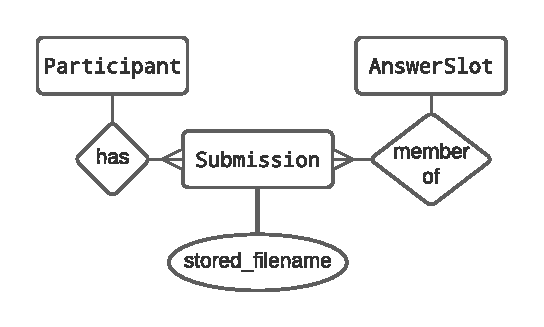
\includegraphics{Gambar/erd-details/ERD--New - Submission.pdf}
        \caption{Potongan diagram relasi entitas untuk \texttt{Submission}.}
        \label{fig:erd_submission}
    \end{figure}

    Entitas \texttt{Submission}, seperti yang dapat dilihat pada potongan
    diagram relasi entitas \ref{fig:erd_submission}, menampung informasi tentang
    submisi yang dilakukan oleh peserta ujian. Submisi yang dikirimkan akan
    disimpan dengan nama berkas yang acak. Nama berkas tersebut kemudian
    disimpan pada database sebagai referensi untuk nantinya pelaporan yang
    dibantu oleh entitas \texttt{ExamReport}.
    
    Submisi yang dikirimkan oleh peserta akan dicek formatnya dengan bantuan
    dari entitas \texttt{AnswerSlot}. Jika nama berkas sudah sesuai dengan
    format, maka data akan dimasukan pada entitas ini.
    
\subsubsection{Notification}
    Entitas \texttt{Notification} menyimpan informasi tentang notifikasi yang
    diberikan pada peserta. Karena beragam notifikasi dapat diberikan pada
    peserta, seperti informasi tentang kredensial untuk masuk ke sistem judge
    atau basis data; atau informasi tentang ralat soal. Oleh karena itu hubungan
    yang dimiliki entitas ini dengan entitas peserta adalah
    \textit{many-to-many}.
    
    Seperti pada diagram relasi entitas pada gambar \ref{fig:erd_overview},
    entitas \texttt{Notification} memiliki beberapa kolom untuk menyimpan isi
    notifikasi (\texttt{description}) dan judul (\texttt{title}). Kolom lainnya,
    seperti \texttt{type} digunakan untuk memasukan notifikasi terhadap grup
    tertentu. Kolom yang terakhir adalah kolom \texttt{extras}. Semua informasi
    yang tidak dapat direpresentasikan pada kolom akan disimpan dalam bentuk
    JSON pada kolom ini. Kolom ini disediakan karna kebutuhan fleksibilitas
    notifikasi yang mungkin akan muncul di masa yang akan datang.

\subsection{Rancangan REST API}
    REST API dirancang dengan pola yang seragam pada beberapa \textit{endpoint}
    besar, sehingga penggunaan API dapat lebih optimal diaplikasikan dengan
    metode abstraksi API class pada sistem frontend.
    
    Perancangan REST API dimulai dengan merancang metode otentikasi yang akan
    digunakan untuk setiap permintaan. Lalu pembahsan dilanjutkan dengan desain
    URL yang digunakan dan tujuannya.
    
    % sistem otentikasi
\subsubsection{Otentikasi API}
    Sesuai dengan kebutuhan, Otentikasi API terbagi menjadi dua bagian besar
    berdasarkan penggunaannya. Otentikasi API yang pertama dilakukan dengan
    menggunakan IP, sedangkan yang kedua, otentikasi dilakukan dengan
    menggunakan token.
    
    Otentikasi dengan IP diperuntukkan untuk API yang berhubungan dengan ujian
    pada lokasi yang telah didefinisikan sebelumnya. IP digunakan karena sistem
    sebelumnya menggunakan cara ini dan telah terbukti pada survei lapangan
    bahwa cara ini sudah sangat efektif. Pengguna tidak perlu melakukan
    otentikasi secara manual dengan memasukkan kredensial khusus untuk sistem.
    Otentikasi dengan IP juga tidak memaksa klien untuk melakukan refresh secara
    terus menerus untuk memperbarui \textit{session} mereka, seperti pada
    aplikasi sebelumnya.
    
    Otentikasi dengan token dilakukan dengan melakukan otentikasi manual hingga
    sistem memberikan sebuah string khusus yang digunakan sebagai token untuk
    setiap permintaan. Otentikasi manual tersebut dapat berupa memasukan
    kredensial login, atau dengan token khusus yang sebelumnya diberikan pada
    email. Token ini nantinya dapat digunakan untuk mengakses berbagai
    \textit{resources} yang backend sediakan. Seperti tombol unduh pada halaman
    laporan, atau melakukan CRUD pada entitas tertentu. Token yang digunakan
    pada sistem normalnya akan menggunakan JSON Web Token atau JWT, dengan
    bantuan \textit{library} dari backend.
    
    % desail url berdasarkan rest API
\subsubsection{Desain \textit{Endpoint}} REST API dibagi menjadi empat bagian
    besar berdasarkan kebutuhannya. Bagian-bagian tersebut memiliki teknik
    otentikasi yang berbeda-beda. Sebagai contoh untuk endpoint otentikasi tidak
    akan memiliki otentikasi sama sekali, atau, otentikasi Ujian dilakukan
    secara tidak langsung dengan menggunakan IP. 
    
    Seluruh endpoint akan memiliki prefiks \texttt{/api/v1/} untuk memberikan
    fleksibilitas di masa yang akan datang pada saat API akan diaplikasikan
    teknik \textit{versioning}. Selain itu, dengan desain url seperti ini,
    pengembang dapat mengetahui versi yang mereka gunakan pada API tersebut.
    
    Pembahasan akan dimulai dengan endpoint untuk otentikasi terlebih dahulu,
    lalu dilanjutkan dengan API ujian, API admin, dan API lainnya.
    
    % Bagian Otentiksi
\subsubsection{Desain \textit{Endpoint} Otentikasi} Endpoint untuk otentikasi
    dapat di akses pada \texttt{system}. Endpoint ini akan bertugas untuk
    menangani segala hal yang berhubungan dengan otentikasi. Mulai dari
    melakukan pengecekan login, mengambil informasi pengguna yang sedang masuk,
    hingga membantu untuk menangani \texttt{IPLogin}. Endpoint ini seharusnya
    bertanggung jawab untuk menerbitkan token JWT berdasarkan informasi pengguna
    terkait yang terekan pada basisdata.
    
    Terdapat satu buah pengecualian untuk otentikasi ujian. Otentikasi ujian
    dilakukan secara tidak langsung dengan melakukan pengecekan IP langsung di
    level endpoint mereka. Endpoint otentikasi tidak akan menerbitkan token
    untuk peserta ujian, karena peserta ujian dapat langsung mengakses endpoint
    \texttt{exam} dengan catatan. IP komputer harus sudah teregistrasi di
    sistem.
    
    Endpoint yang digunakan untuk otentikasi terdiri dari:
    \begin{itemize}
        \item \texttt{POST auth/login} \\
            Bertanggung jawab untuk melakukan login, membangkitkan token, serta
            memberi informasi singkat tentang pengguna yang masuk.\\
            \textbf{Input:}
            \begin{itemize}
                \item \texttt{username}: \textit{string}, Nama pengguna atau
                    email.
                \item \texttt{password}: \textit{string}, Kata sandi pengguna.
            \end{itemize}
            \textbf{Output:}
            \begin{itemize}
                \item \texttt{id\_token}: \textit{string}, Token otentikasi.
                \item \texttt{profile}: \textit{object}, objek dari entitas
                    \texttt{User}.
            \end{itemize}
        
        \item \texttt{POST auth/iplogin} \\
            Bertanggung jawab untuk melakukan login dengan IP, membangkitkan
            token, serta memberi informasi singkat tengang pengguna yang tertau
            dengan IP tersebut. \\
            \textbf{Input:} -\\
            \textbf{Output:}
            \begin{itemize}
                \item \texttt{id\_token}: \textit{string}, Token otentikasi.
                \item \texttt{profile}: \textit{object}, objek dari entitas
                    \texttt{User}.
            \end{itemize}
            
        \item \texttt{GET user/me} \\
            Bertanggung jawab untuk memberikan informasi tentang user yang
            terautentikasi. \textbf{Input:} -\\
            \textbf{Output:}
            \begin{itemize}
                \item \texttt{profile}: \textit{object}, objek dari entitas
                    \texttt{User}.
            \end{itemize}
            
        \item \texttt{POST user/me} \\
            Bertanggung jawab untuk memperbarui informasi tentang user yang
            terautentikasi. \textbf{Input:} Objek dari entitas \texttt{User}.\\
            \textbf{Output:}
            \begin{itemize}
                \item \texttt{profile}: \textit{object}, objek dari entitas
                    \texttt{User}.
            \end{itemize}
    \end{itemize}
    
    % Bagian Exam
\subsubsection{Desain \textit{Endpoint} Ujian} Endpoint untuk ujian memiliki
    prefiks \texttt{exam}. Endpoint ini akan menggunakan otentikasi IP dan tidak
    membutuhkan penggunanya untuk mengirimkan informasi header
    \textit{Authorization} apapun. Endpoint ini akan melayani segala kebutuhan
    peserta untuk ujian.
    
    Endpoint yang melayani API untuk ujian terdiri dari:
    \begin{itemize}
        \item \texttt{GET info} \\
            Bertanggung jawab untuk mengembalikan informasi ujian yang sedang
            dan akan dimulai. \\
            \textbf{Input:} -\\
            \textbf{Output:} objek dari entitas \texttt{Participant}

        \item \texttt{GET notification} \\
            Bertanggung jawab untuk mengembalikan daftar notifikasi.\\
            \textbf{Input:} -\\
            \textbf{Output:} \textit{array} objek entitas \texttt{Notifikasi}

        \item \texttt{GET submission} \\
            Bertanggung jawab untuk mengembalikan status submisi pada slot
            jawaban tertentu.\\
            \textbf{Input:} -\\
            \textbf{Output:} objek dari entitas \texttt{Submission}

        \item \texttt{POST submission} \\
            Bertanggung jawab untuk mengirimkan berkas jawaban (selanjutnya
            disebut submisi) pada slot jawaban tertentu.\\
            \textbf{Input:} \begin{itemize}
                \item \texttt{file}: \textit{multipart-form}, berkas ujian dalam
                    bentuk blob.
                \item \texttt{answer\_slot}: \textit{string|number}, id dari
                    slot jawaban yang akan disubmisi.
            \end{itemize}
            \textbf{Output:} objek dari entitas \texttt{Submission}
    \end{itemize}
    
    % Bagian Admin
\subsubsection{Desain \textit{Endpoint} Admin} Slot endpoint yang digunakan
    untuk admin mengatur berbagai fitur yang tersedia pada admin panel. Endpoint
    ini membutuhan otentikasi pengguna level admin. Setiap entitas memiliki
    tabel izinnya masing-masing yang dapat diperoleh dari entitas
    \texttt{AclItem}. Namun pada dasarnya, setiap admin berhak untuk melakukan
    \texttt{CRUD} pada entitas tersebut, kecuali disebutkan sebaliknya.
    
    Enpoin pada admin ini memiliki prefiks \texttt{manage}. Karena enpoint ini
    berhubungan langsung dengan entitas, maka pada dasarnya seluruh entitas
    memiliki endpoint khusus dengan pola REST API sebagai berikut
    \begin{itemize}
        \item \texttt{GET :entity} \\
            Bertanggung jawab untuk mengembalikan daftar entri dari
            \texttt{:entity} yang disebutkan.\\
            \textbf{Input:} -\\
            \textbf{Output:} \textit{array} objek entitas \texttt{:entity}
            
        \item \texttt{POST :entity} \\
            Bertanggung jawab untuk membuat entri baru dari \texttt{:entity}
            yang disebutkan.\\
            \textbf{Input:} objek (atau beberapa bagian} dari entitas
                \texttt{:entity}.\\
            \textbf{Output:} objek dari entitas \texttt{:entity}.
            
        \item \texttt{GET :entity/:id} \\
            Bertanggung jawab untuk mengembalikan info detil entri dari
            \texttt{:entity} dengan id \texttt{:id}.\\
            \textbf{Input:} -\\
            \textbf{Output:} objek dari entitas \texttt{:entity}
            
        \item \texttt{PUT :entity/:id} \\
            Bertanggung jawab untuk mengubah atau memperbarui entri dengan id
            \texttt{:id} pada entitas \texttt{entity}.\\
            \textbf{Input:} objek atau beberapa bagian) dari entitas
                \texttt{:entity}.\\
            \textbf{Output:} objek dari entitas \texttt{:entity}
        
        \item \texttt{DELETE :entity/:id} \\
            Bertanggung jawab untuk menghapus entri \texttt{:id} pada
            \texttt{entity}.\\
            \textbf{Input:} -\\
            \textbf{Output:} objek dari entitas \texttt{:entity}.
    \end{itemize}
    
    Selain dari pola tersebut, terdapat beberapa endpoint khusus untuk
    memfasilitasi aksi yang dapat dilakukan pada entitas tersebut. Endpoint
    tersebut adalah
    \begin{itemize}
        \item \texttt{DELETE exam/:id/start} \\
            Bertanggung jawab untuk melakukan reset timer ujian pada id
            tertentu.\\
            \textbf{Input:} -\\
            \textbf{Output:} \textit{object} objek entitas \texttt{Exam}.
            
        \item \texttt{GET exam/:id/answers} \\
            Bertanggung jawab untuk melakukan pengumpulan jawaban dan
            pengunduhan dalam bentuk zip.\\
            \textbf{Input:} -\\
            \textbf{Output:} \textit{blob} berkas zip.
            
        \item \texttt{GET exam/:id/notifications} \\
            Bertanggung jawab untuk mengembalikan daftar notifikasi yang tertaut
            pada peserta di ujian yang disebutkan.\\
            \textbf{Input:} -\\
            \textbf{Output:} \textit{array} objek entitas \texttt{Notification}.
            
        \item \texttt{GET exam/:id/participants} \\
            Bertanggung jawab untuk mengembalikan daftar peserta yang terdapat
            pada ujian ini.\\
            \textbf{Input:} -\\
            \textbf{Output:} \textit{array} objek entitas \texttt{Participant}.
            
        \item \texttt{GET exam/:id/script} \\
            Bertanggung jawab untuk membuat \textit{script} yang digunakan untuk
            membuat lembar kerja peserta ujian.\\
            \textbf{Input:} -\\
            \textbf{Output:} \textit{blob} berkas zip.
            
        \item \texttt{POST exam/:id/close} \\
            Bertanggung jawab untuk menghentikan timer ujian dan menutup lembar
            jawab peserta secara manual.\\
            \textbf{Input:} -\\
            \textbf{Output:} \textit{object} objek entitas \texttt{Exam}.
            
        \item \texttt{POST exam/:id/move} \\
            Bertanggung jawab untuk memindahkan peserta ke tempat duduk lain dan
            membuat \textit{script} untuk lembar kerja mahasiswa yang baru.\\
            \textbf{Input:} \begin{itemize}
                \item \texttt{lists[].participant}: \textit{string|id}, id dari
                peserta.
                \item \texttt{lists[].to}: \textit{string|id}, id dari komputer
                target.
            \end{itemize}
            \textbf{Output:} \textit{blob} berkas zip.
            
        \item \texttt{POST exam/:id/populate} \\
            Bertanggung jawab untuk melakukan populasi tempat duduk yang sudah
            dipilih dengan daftar peserta yang ada.\\
            \textbf{Input:} \begin{itemize}
                \item \texttt{computers}: \textit{array} id dari entitas
                    \texttt{Computer}.
                \item \texttt{participants}: \textit{array} id dari entitas
                    \texttt{Participant}.
                \item \texttt{should\_cleanup}: \textit{boolean} Hapus daftar
                    peserta yang sudah ada.
            \end{itemize}
            \textbf{Output:} objek dari entitas \texttt{Exam}.
            
        \item \texttt{POST exam/:id/start} \\
            Bertanggung jawab untuk memulai timer pada ujian.\\
            \textbf{Input:} -\\
            \textbf{Output:} \textit{object} objek entitas \texttt{Exam}.
            
        \item \texttt{POST examreport/:id/forcesend} \\
            Bertanggung jawab untuk melakukan pengiriman laporan ujian secara
            paksa ke email yang terdapat pada entri \texttt{:id}.\\
            \textbf{Input:} -\\
            \textbf{Output:} -
            
        \item \texttt{POST notification/mass\_gen} \\
            Bertanggung jawab untuk melakukan penyebaran notifikasi kata sandi
            pada daftar yang diberikan pada ujian tertentu.\\
            \textbf{Input:} \begin{itemize}
                \item \texttt{lists[].participant}: \textit{string|id} id dari
                    entitas \texttt{Participant}.
                \item \texttt{lists[].username}: \textit{string} Nama pengguna
                layanan
                \item \texttt{lists[].password}: \textit{string} Kata sandi
                layanan
                \item \texttt{url}: \textit{string} Alamat layanan
            \end{itemize}
            \textbf{Output:} -
    \end{itemize}
    
    % Bagian Dosen
\subsubsection{Desain \textit{Endpoint} Lainnya} Endpoint lainnya terdiri dari
    endpoint yang dapat digunakan dengan otentikasi khusus. Otentikasi tersebut
    dapat dengan menukarkan token \textit{payload} tertentu menjadi token bentuk
    lain. Endpoint tersebut terdiri dari
    \begin{itemize}
        \item \texttt{POST autonomus/examdownload} \\
            Endpoint ini bertanggung jawab untuk mengembalikan informasi tentang
            token yang terhubung dengan ujian tertentu, serta memberikan link
            otorisasi pengunduhan berkas jawaban.\\
            \textbf{Input:} \begin{itemize}
                \item \texttt{token}: \textit{string}, token dari laporan ujian
                    yang dikirimkan via email.
            \end{itemize}
            \textbf{Output:} \begin{itemize}
                \item \texttt{exam}: \textit{object}, objek dari entitas
                \texttt{Exam}.
                \item \texttt{downloadToken}: \textit{string}, tautan lengkap
                    untuk mengunduh ujian.
            \end{itemize}
            
        \item \texttt{GET autonomus/examdownload/download} \\
            Endpoint ini bertanggung jawab untuk menyediakan berkas jawaban
            dalam bentuk zip.\\
            \textbf{Input:} -\\
            \textbf{Output:} \textit{blob} berkas zip.
    \end{itemize}
    
    % diagram kelas
\subsection{Desain Kelas}
    \begin{figure}
        \centering
        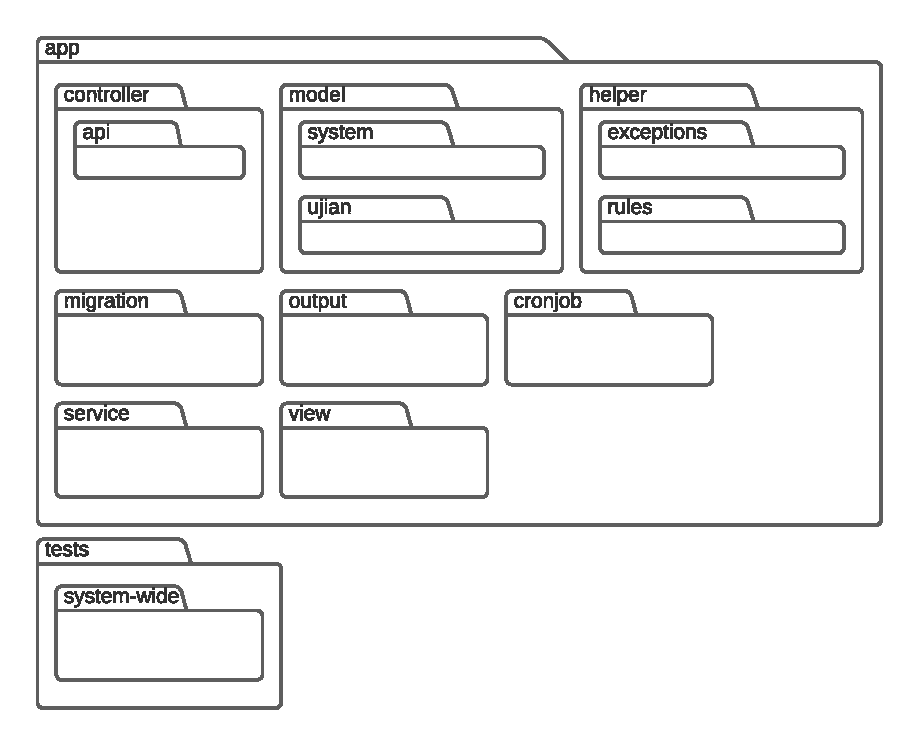
\includegraphics{Gambar/classmap-be/Classmap - Overview.pdf}
        \caption{Gambaran besar dari perancangan kelas untuk sistem
        \textit{back-end}.}
        \label{fig:classmap_overview}
    \end{figure}
    Perancangan desain kelas dilakukan dengan mempertimbangkan pola yang telah
    diberikan oleh beberapa \textit{library}. Karena \textit{framework} yang
    digunakan cukup fleksibel, maka dibuat beberapa \textit{namespace} sesuai
    dengan konteks penggunaan kelasnya masing-masing. Secara garis besar,
    \textit{namespace} yang ada aplikasi dapat dilihat pada Gambar
    \ref{fig:classmap_overview}.
    
    Kemudian setiap \textit{namespace} akan dijelaskan secara terperinci beserta
    dengan kelas yang terdapat pada \textit{namespace} tersebut.

\subsubsection{\textit{Namespace} \texttt{Controller}}
    
    \begin{figure}
        \centering
        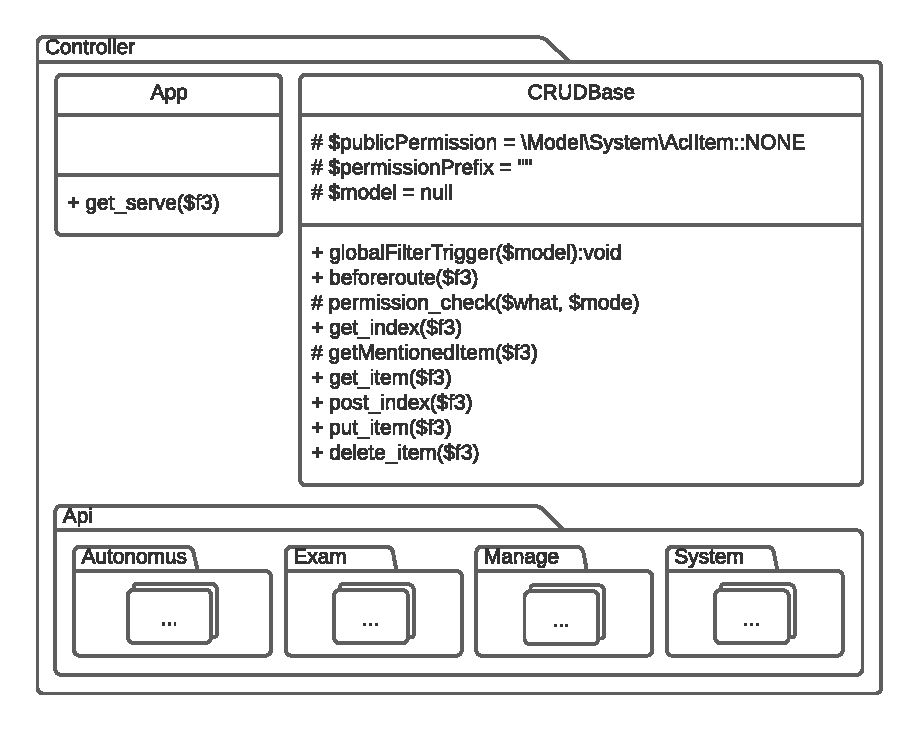
\includegraphics{Gambar/classmap-be/Classmap - app-controller.pdf}
        \caption{Diagram kelas untuk \textit{namespace} \texttt{Controller}.}
        \label{fig:classmap_app-controller}
    \end{figure}

    \textit{Namespace} ini akan berisi kelas-kelas yang bertanggung jawab untuk
    menangani permintaan. Permintaan tersebut terdiri dari permintaan dari API
    dan permintaan non-API. Diagram kelas untuk \textit{namespace} ini dapat
    diperhatikan pada Gambar
    \ref{fig:classmap_app-controller}
    
    \textit{Namespace} ini terdiri dari kelas-kelas berikut:
    \begin{itemize}
        \item \texttt{App} \\
            Kelas ini bertanggung jawab untuk menyajikan aplikasi React. Oleh
            karena itu sesuai dengan desain rutenya, kelas ini akan menangani
            permintaan pada \textit{url}:
            \begin{itemize}
                \item \texttt{GET /admin}
                \item \texttt{GET /admin/*}
                \item \texttt{GET /exam}
                \item \texttt{GET /exam/*}
                \item \texttt{GET /autonomus}
                \item \texttt{GET /autonomus/*}
            \end{itemize}
            Definisi rute lengkap URL dapat dilihat pada lampiran (TODO:
            lampiran routings.ini).
            
            Pada kelas ini terdapat fungsi:
            \begin{itemize}
                \item \texttt{get\_serve(\$f3)} \\
                    Fungsi ini yang bertanggung jawab untuk menyajikan aplikasi
                    React.\\
                    \textbf{Input:} Instansi kelas \texttt{Base} dari framework.
                    \\
                    \textbf{Output:} -
            \end{itemize}
        
        \item  \texttt{CRUDBase} \\
            Kelas ini akan menjadi kelas yang menangani abstraksi dari REST API.
            Atribut yang terdapat pada kelas ini adalah:
            \begin{itemize}
                \item \texttt{\$publicPermission}\\
                    Mendefinisikan permisi yang dimiliki oleh pengkonsumsi API
                    tanpa otentikasi.
                \item \texttt{\$permissionPrefix}\\
                    Mendefinisikan nama permisi yang tertaut pada pengkonsumsi
                    API yang terotentikasi.
                \item \texttt{\$model}\\
                    Mendefinisikan nama kelas model yang akan digunakan. Nama
                    kelas yang diharapkan adalah \textit{fully qualified
                    name}\footnote{Lihat
                    https://www.php.net/manual/en/language.namespaces.rules.php}.
            \end{itemize}
            Fungsi yang terdapat pada kelas ini adalah:
            \begin{itemize}
                \item \texttt{globalFilterTrigger(\$model):void} \\
                    Menangani filter global untuk model yang ditautkan untuk
                    kelas ini. \\
                    \textbf{Input:} instansi model\\
                    \textbf{Output:} -
                
                \item \texttt{beforeroute(\$f3)}\\
                    Menangani \textit{event} sebelum \textit{framework}
                    melakukan pemanggilan fungsi utama.\\
                    \textbf{Input:} Instansi kelas \texttt{Base} dari
                    framework.\\
                    \textbf{Output:} -
                    
                \item \texttt{permission\_check(\$what, \$mode)} \\
                    Melakukan pengecekan permisi/izin pada otentikasi
                    pengkonsumsi API. Mungkin akan melempar eksepsi jika
                    pengkonsumsi tidak memiliki izin.\\
                    \textbf{Input:} Nama permisi, dan mode yang seharusnya
                        diperbolehkan (buat, baca, ubah, hapus)\\
                    \textbf{Output:} -
                
                \item \texttt{get\_index(\$f3)} \\
                    Menangani permintaan API untuk melakukan \textit{listinig}
                    entri dari model \\
                    \textbf{Input:} Instansi kelas \texttt{Base} dari
                    framework.\\
                    \textbf{Output:} -
                
                \item \texttt{getMentionedItem(\$f3)} \\
                    Ambil entri yang disebutkan pada \textit{url}. \\
                    \textbf{Input:} Instansi kelas \texttt{Base} dari
                    framework.\\
                    \textbf{Output:} Instansi model yang tertaut dengan sebuah
                    entri.
                
                \item \texttt{get\_item(\$f3)} \\
                    Menangani permintaan API untuk menampilan infomasi lengkap
                    entri. \\
                    \textbf{Input:} Instansi kelas \texttt{Base} dari
                    framework.\\
                    \textbf{Output:} -
                
                \item \texttt{post\_index(\$f3)} \\
                    Menangani permintaan API untuk membuat entri baru. \\
                    \textbf{Input:} Instansi kelas \texttt{Base} dari
                    framework.\\
                    \textbf{Output:} -
                
                \item \texttt{put\_item(\$f3)} \\
                    Menangani permintaan API untuk memperbarui/mengubah
                    informasi pada entri. \\
                    \textbf{Input:} Instansi kelas \texttt{Base} dari
                    framework.\\
                    \textbf{Output:} -
                
                \item \texttt{delete\_item(\$f3)} \\
                    Menagnagi permintaa API untuk menghapus entri. \\
                    \textbf{Input:} Instansi kelas \texttt{Base} dari
                    framework.\\
                    \textbf{Output:} -
            \end{itemize}
    \end{itemize}
    
    \begin{figure}
        \centering
        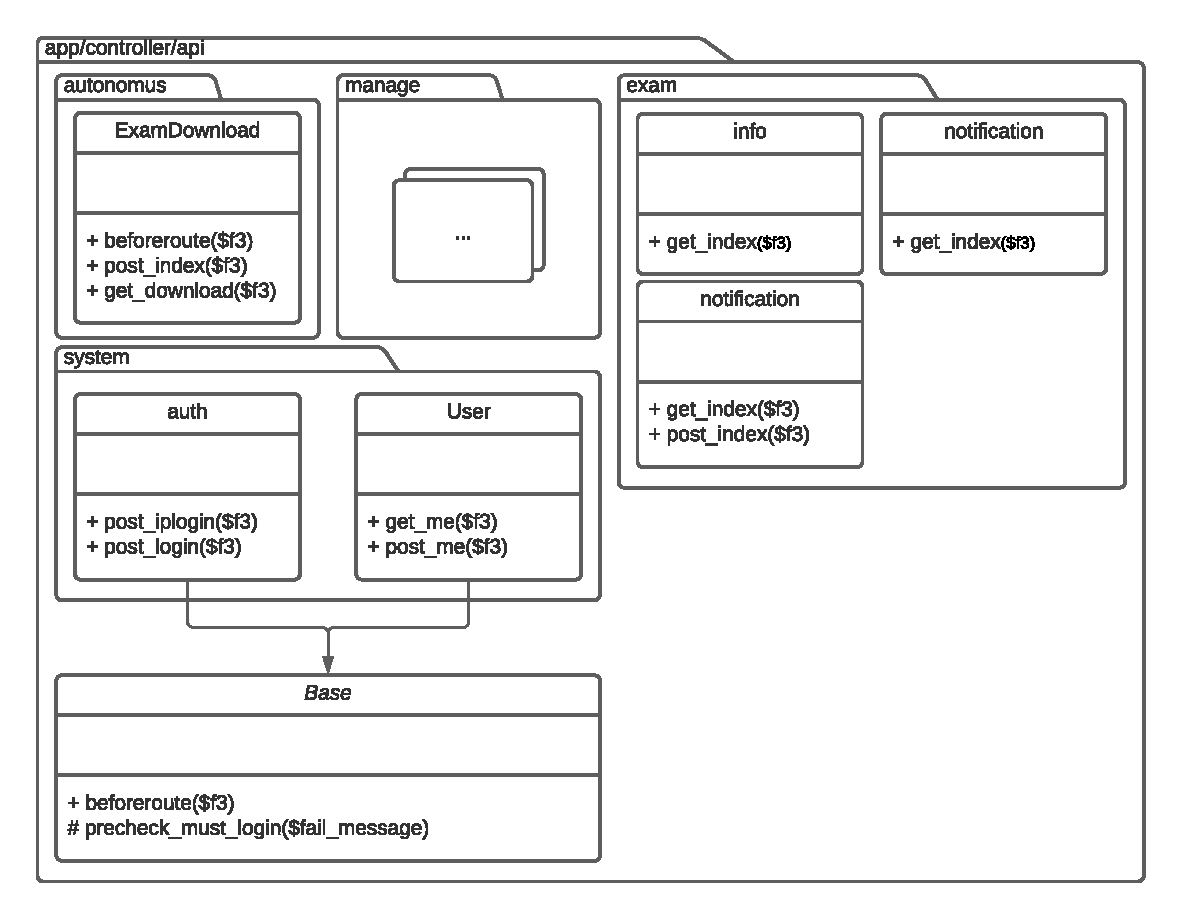
\includegraphics[width=0.75\paperwidth]{Gambar/classmap-be/Classmap - app-controller-api.pdf}
        \caption{Potongan diagram kelas untuk \textit{namespace}
        \texttt{Controller/Api}.}
        \label{fig:classmap_app-controller-api}
    \end{figure}
    
    Selain dari kelas-kelas tersebut, \textit{namespace} ini memiliki anak
    \textit{namespace} \texttt{Api}. \textit{Namespace} tersebut secara gais
    besar akan menangani berbagai macam permintaan API yang akan disediakan oleh
    sistem \textit{back-end}. Diagram kelas untuk \textit{namespace} ini dapat
    dilihat pada Gambar \ref{fig:classmap_app-controller-api}.
    
    \textit{Namespace} \texttt{Api} terdiri dari:
    \begin{itemize}
        \item \texttt{Base} \\
            Kelas ini bertanggung jawab untuk menangani abstraksi API dasar yang
            diperlukan. Kelas ini memiliki fungsi:
            \begin{itemize}
                \item \texttt{beforeroute(\$f3)} \\
                    Menangani \textit{event} sebelum \textit{framework}
                    melakukan pemanggilan fungsi utama. Melakukan parsing dan
                    pengecekan tertentu pada permintaan API.\\
                    \textbf{Input:} Instansi kelas \texttt{Base} dari framework.
            \end{itemize}
    
        \item \texttt{Autonomus\textbackslash ExamDownload} \\
            Kelas ini bertanggung jawab untuk melayani API untuk pengunduhan
            jawaban via tautan yang dikirimkan ke email. Kelas ini memiliki
            fungsi:
            \begin{itemize}
                \item \texttt{beforeroute(\$f3)} \\
                    Menangani \textit{event} sebelum \textit{framework}
                    melakukan pemanggilan fungsi utama.\\
                    \textbf{Input:} Instansi kelas \texttt{Base} dari
                    framework.\\
                    \textbf{Output:} -
                
                \item \texttt{post\_index(\$f3)} \\
                    Menangani penukaran token dengan informasi ujian dan
                    menerbitkan tautan untuk melakukan pengunduhan.\\
                    \textbf{Input:} Instansi kelas \texttt{Base} dari
                    framework.\\
                    \textbf{Output:} - \\
                    \textbf{URL:} \texttt{POST autonomus/examdownload}
                
                \item \texttt{get\_download(\$f3)} \\
                    Menyediakan layanan pengunduhan berkas berupa Zip.
                    \textbf{Input:} Instansi kelas \texttt{Base} dari
                    framework.\\
                    \textbf{Output:} -\\
                    \textbf{URL:} \texttt{GET autonomus/examdownload/download}
            \end{itemize}
            
        \item \texttt{Exam\textbackslash Info} \\
            Bertanggung jawab untuk memberikan informasi tentang ujian yang
            tertaut pada IP pengkonsumsi API pada waktu tertentu. Kelas ini
            memiliki fungsi:
            \begin{itemize}
                \item \texttt{get\_index(\$f3)} \\
                    Memberikan informasi tentang ujian yang sedang aktif.
                    \textbf{Input:} Instansi kelas \texttt{Base} dari
                    framework.\\
                    \textbf{Output:} - \\
                    \textbf{URL:} \texttt{GET exam/info}
            \end{itemize}
            
        \item \texttt{Exam\textbackslash Notification} \\
            Bertanggung jawab untuk memberikan notifikasi yang tertaut dengan
            peserta yang sedang aktif. Kelas ini memiliki fungsi:
            \begin{itemize}
                \item \texttt{get\_index(\$f3)} \\
                    Memberikan daftar entri notifikasi. \textbf{Input:} Instansi
                    kelas \texttt{Base} dari framework.\\
                    \textbf{Output:} -\\
                    \textbf{URL:} \texttt{GET exam/notification}
            \end{itemize}
            
        \item \texttt{Exam\textbackslash Submission} \\
            Bertanggung jawab untuk menangi berbagai hal seputar submisi
            peserta. Kelas ini memiliki fungsi:
            \begin{itemize}
                \item \texttt{get\_index(\$f3)} \\
                    Memberikan informasi tentang submisi pada slot jawaban
                    tertentu. \textbf{Input:} Instansi kelas \texttt{Base} dari
                    framework.\\
                    \textbf{Output:} -\\
                    \textbf{URL:} \texttt{GET exam/submission}
                    
                \item \texttt{get\_index(\$f3)} \\
                    Menangani submisi yang dikirimkan peserta pada slot jawaban
                    tertentu. \textbf{Input:} Instansi kelas \texttt{Base} dari
                    framework.\\
                    \textbf{Output:} -\\
                    \textbf{URL:} \texttt{POST exam/submission}
            \end{itemize}
            
        \item \texttt{System\textbackslash Auth} \\
            Bertanggung jawab untuk menangi berbagai hal seputar otentikasi
            dengan kata sandi dan nama pengguna.
            \begin{itemize}
                \item \texttt{post\_iplogin(\$f3)}\\
                    Menangani permintaan untuk login dengan menggunakan IP.\\
                    \textbf{Input:} Instansi kelas \texttt{Base} dari
                    framework.\\
                    \textbf{Output:} -\\
                    \textbf{URL:} \texttt{POST system/auth/iplogin}
                
                \item \texttt{post\_login(\$f3)}\\
                    Menangani permitnaan untuk login dengan mengguankan
                    kombinasi nama pengguna atau email, dan kata sandi.\\
                    \textbf{Input:} Instansi kelas \texttt{Base} dari
                    framework.\\
                    \textbf{Output:} -\\
                    \textbf{URL:} \texttt{POST system/auth/login}
            \end{itemize}

        \item \texttt{System\textbackslash User} \\
            Bertanggung jawab untuk menangi berbagai hal seputar otentikasi
            dengan kata sandi dan nama pengguna.
            \begin{itemize}
                \item \texttt{get\_me(\$f3)}\\
                    Menangani permintaan informasi tentang user itu sendiri.\\
                    \textbf{Input:} Instansi kelas \texttt{Base} dari
                    framework.\\
                    \textbf{Output:} -\\
                    \textbf{URL:} \texttt{GET system/user/me}
                
                \item \texttt{post\_me(\$f3)}\\
                    Menangani permintaan untuk mengubah informasi tentang user
                    itu sendiri .\\
                    \textbf{Input:} Instansi kelas \texttt{Base} dari
                    framework.\\
                    \textbf{Output:} -\\
                    \textbf{URL:} \texttt{POST system/user/me}
                    
            \end{itemize}
    \end{itemize}
    
    \begin{sidewaysfigure}
        \centering
        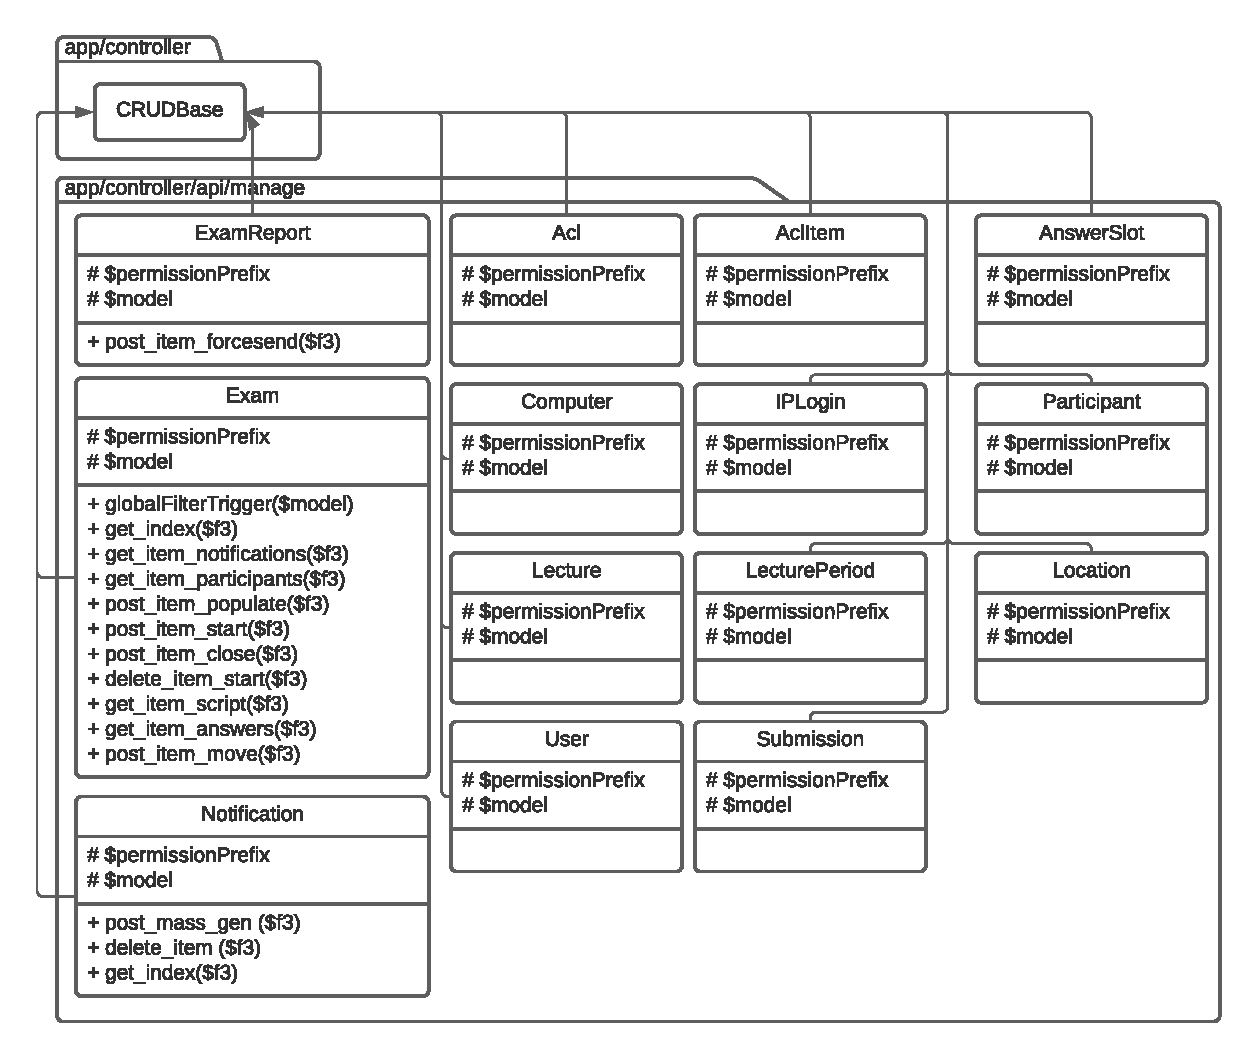
\includegraphics{Gambar/classmap-be/Classmap - app-controller-api-manage.pdf}
        \caption{Potongan diagram kelas untuk \textit{namespace}
        \texttt{Controller/Api/Manage}.}
        \label{fig:classmap_app-controller-api-manage}
    \end{sidewaysfigure}
    Kemudian terdapat kelas-kelas dari \textit{namespace}
    \texttt{Controller/Api/Manage} yang memiliki banyak kelas turunan dari
    \texttt{CRUDBase}. Diagram kelas tersebut dapat dilihat pada Gambar
    \ref{fig:classmap_app-controller-api-manage}. \textit{Namespace} tersebut
    memiliki kelas-kelas berikut:
    \begin{itemize}
        \item \texttt{Acl}\\
            Bertanggung jawab untuk menangani permintaan REST API untuk entitas
            \texttt{Acl}. Kelas ini memiliki atribut:
            \begin{itemize}
                \item \texttt{\$permissionPrefix}: Turunan dari kelas
                \texttt{CRUDBase}.
                \item \texttt{\$model}: Turunan dari kelas \texttt{CRUDBase}.
            \end{itemize}
        
        \item \texttt{AclItem}\\
            Bertanggung jawab untuk menangani permintaan REST API untuk entitas
            \texttt{AclItem}. Kelas ini memiliki atribut:
            \begin{itemize}
                \item \texttt{\$permissionPrefix}: Turunan dari kelas
                \texttt{CRUDBase}.
                \item \texttt{\$model}: Turunan dari kelas \texttt{CRUDBase}.
            \end{itemize}
        
        \item \texttt{AnswerSlot}\\
            Bertanggung jawab untuk menangani permintaan REST API untuk entitas
            \texttt{AnswerSlot}. Kelas ini memiliki atribut:
            \begin{itemize}
                \item \texttt{\$permissionPrefix}: Turunan dari kelas
                \texttt{CRUDBase}.
                \item \texttt{\$model}: Turunan dari kelas \texttt{CRUDBase}.
            \end{itemize}
        
        \item \texttt{Computer}\\
            Bertanggung jawab untuk menangani permintaan REST API untuk entitas
            \texttt{Computer}. Kelas ini memiliki atribut:
            \begin{itemize}
                \item \texttt{\$permissionPrefix}: Turunan dari kelas
                \texttt{CRUDBase}.
                \item \texttt{\$model}: Turunan dari kelas \texttt{CRUDBase}.
            \end{itemize}
        
        \item \texttt{IPLogin}\\
            Bertanggung jawab untuk menangani permintaan REST API untuk entitas
            \texttt{IPLogin}. Kelas ini memiliki atribut:
            \begin{itemize}
                \item \texttt{\$permissionPrefix}: Turunan dari kelas
                \texttt{CRUDBase}.
                \item \texttt{\$model}: Turunan dari kelas \texttt{CRUDBase}.
            \end{itemize}
        
        \item \texttt{Participant}\\
            Bertanggung jawab untuk menangani permintaan REST API untuk entitas
            \texttt{Participant}. Kelas ini memiliki atribut:
            \begin{itemize}
                \item \texttt{\$permissionPrefix}: Turunan dari kelas
                \texttt{CRUDBase}.
                \item \texttt{\$model}: Turunan dari kelas \texttt{CRUDBase}.
            \end{itemize}
        
        \item \texttt{Lecture}\\
            Bertanggung jawab untuk menangani permintaan REST API untuk entitas
            \texttt{Lecture}. Kelas ini memiliki atribut:
            \begin{itemize}
                \item \texttt{\$permissionPrefix}: Turunan dari kelas
                \texttt{CRUDBase}.
                \item \texttt{\$model}: Turunan dari kelas \texttt{CRUDBase}.
            \end{itemize}
        
        \item \texttt{LecturePeriod}\\
            Bertanggung jawab untuk menangani permintaan REST API untuk entitas
            \texttt{LecturePeriod}. Kelas ini memiliki atribut:
            \begin{itemize}
                \item \texttt{\$permissionPrefix}: Turunan dari kelas
                \texttt{CRUDBase}.
                \item \texttt{\$model}: Turunan dari kelas \texttt{CRUDBase}.
            \end{itemize}
        
        \item \texttt{Location}\\
            Bertanggung jawab untuk menangani permintaan REST API untuk entitas
            \texttt{Location}. Kelas ini memiliki atribut:
            \begin{itemize}
                \item \texttt{\$permissionPrefix}: Turunan dari kelas
                \texttt{CRUDBase}.
                \item \texttt{\$model}: Turunan dari kelas \texttt{CRUDBase}.
            \end{itemize}
        
        \item \texttt{User}\\
            Bertanggung jawab untuk menangani permintaan REST API untuk entitas
            \texttt{User}. Kelas ini memiliki atribut:
            \begin{itemize}
                \item \texttt{\$permissionPrefix}: Turunan dari kelas
                \texttt{CRUDBase}.
                \item \texttt{\$model}: Turunan dari kelas \texttt{CRUDBase}.
            \end{itemize}
        
        \item \texttt{Submission}\\
            Bertanggung jawab untuk menangani permintaan REST API untuk entitas
            \texttt{Submission}. Kelas ini memiliki atribut:
            \begin{itemize}
                \item \texttt{\$permissionPrefix}: Turunan dari kelas
                \texttt{CRUDBase}.
                \item \texttt{\$model}: Turunan dari kelas \texttt{CRUDBase}.
            \end{itemize}
        
        \item \texttt{ExamReport}\\
            Bertanggung jawab untuk menangani permintaan REST API untuk entitas
            \texttt{ExamReport}. Kelas ini memiliki atribut:
            \begin{itemize}
                \item \texttt{\$permissionPrefix}: Turunan dari kelas
                \texttt{CRUDBase}.
                \item \texttt{\$model}: Turunan dari kelas \texttt{CRUDBase}.
            \end{itemize}
            Selain itu, kelas ini memiliki fungsi:
            \begin{itemize}
                \item \texttt{post\_item\_forcesend(\$f3)} \\
                    Bertanggung jawab untuk mengirimkan laporan ke email yang
                    terdapat pada entri secara manual.\\
                    \textbf{Input:} Instansi kelas \texttt{Base} dari
                    framework.\\
                    \textbf{Output:} -\\
                    \textbf{URL:} \texttt{POST manage/examreport/:id/forcesend}
            \end{itemize}
        
        \item \texttt{Exam}\\
            Bertanggung jawab untuk menangani permintaan REST API untuk entitas
            \texttt{Exam}. Kelas ini memiliki atribut:
            \begin{itemize}
                \item \texttt{\$permissionPrefix}: Turunan dari kelas
                \texttt{CRUDBase}.
                \item \texttt{\$model}: Turunan dari kelas \texttt{CRUDBase}.
            \end{itemize}
            Selain itu, kelas ini memiliki fungsi:
            \begin{itemize}
                \item \texttt{globalFilterTrigger(\$model)} \\
                    Diturunkan dari kelas \textit{CRUDBase}. Digunakan untuk
                    melimitasi daftar entri yang dikembalikan khusus untuk
                    pengkonsumsi API yang terotentikasi via IPLogin. \\
                    \textbf{Input:} Instansi dari model yang ditautkan ke kelas
                    ini.\\
                    \textbf{Output:} -
                
                \item \texttt{get\_index(\$f3)} \\
                    Meng\textit{override} fungsi dari kelas \textit{CRUDBase}.
                    Digunakan untuk menampilkan subset dengan kueri khusus untuk
                    pengkonsumsi API yang terotentikasi via IPLogin.\\
                    \textbf{Input:} Instansi kelas \texttt{Base} dari
                    framework.\\
                    \textbf{Output:} -\\
                    \textbf{URL:} \texttt{GET manage/exam/:id}
                
                \item \texttt{get\_item\_notifications(\$f3)} \\
                    Menangani permintaan untuk mengembalikan daftar notifikasi
                    yang terhubung dengan peserta yang mengikuti ujian ini.\\
                    \textbf{Input:} Instansi kelas \texttt{Base} dari
                    framework.\\
                    \textbf{Output:} -\\
                    \textbf{URL:} \texttt{GET manage/exam/:id/notifications}
                
                \item \texttt{get\_item\_participants(\$f3)} \\
                    Menangani permintaan untuk mengembalikan daftar peserta yang
                    terhubung dengan ujian ini.\\
                    \textbf{Input:} Instansi kelas \texttt{Base} dari
                    framework.\\
                    \textbf{Output:} -\\
                    \textbf{URL:} \texttt{GET manage/exam/:id/participants}
                
                \item \texttt{post\_item\_populate(\$f3)} \\
                    Melakukan populasi tempat duduk dengan daftar peserta
                    ujian.\\
                    \textbf{Input:} Instansi kelas \texttt{Base} dari
                    framework.\\
                    \textbf{Output:} -\\
                    \textbf{URL:} \texttt{POST manage/exam/:id/populate}
                
                \item \texttt{post\_item\_start(\$f3)} \\
                    Bertanggung jawab untuk memulai timer.\\
                    \textbf{Input:} Instansi kelas \texttt{Base} dari
                    framework.\\
                    \textbf{Output:} -\\
                    \textbf{URL:} \texttt{POST manage/exam/:id/start}
                
                \item \texttt{post\_item\_close(\$f3)} \\
                    Bertanggung jawab utnuk menutup timer.\\
                    \textbf{Input:} Instansi kelas \texttt{Base} dari
                    framework.\\
                    \textbf{Output:} -\\
                    \textbf{URL:} \texttt{POST manage/exam/:id/close}
                
                \item \texttt{delete\_item\_start(\$f3)} \\
                    Bertanggung jawab untuk menyetel ulang timer.\\
                    \textbf{Input:} Instansi kelas \texttt{Base} dari
                    framework.\\
                    \textbf{Output:} -\\
                    \textbf{URL:} \texttt{DELETE manage/exam/:id/start}
                
                \item \texttt{get\_item\_script(\$f3)} \\
                    Menangani pembuatan \textit{script} untuk membuat lembar
                    kerja ujian peserta dan menyalin berkas pendukung ujian ke
                    komputer peserta.\\
                    \textbf{Input:} Instansi kelas \texttt{Base} dari
                    framework.\\
                    \textbf{Output:} -\\
                    \textbf{URL:} \texttt{GET manage/exam/:id/script}
                    
                \item \texttt{get\_item\_answers(\$f3)} \\
                    Bertanggung jawab untuk mengumpulkan jawaban, lalu
                    menggabungkannya dalam sebuah \textit{archive} zip.\\
                    \textbf{Input:} Instansi kelas \texttt{Base} dari
                    framework.\\
                    \textbf{Output:} -\\
                    \textbf{URL:} \texttt{GET manage/exam/:id/answers}
                
                \item \texttt{post\_item\_move(\$f3)} \\
                    Menangani pemindahan peserta pada komputer tertentu.\\
                    \textbf{Input:} Instansi kelas \texttt{Base} dari
                    framework.\\
                    \textbf{Output:} -\\
                    \textbf{URL:} \texttt{POST manage/exam/:id/move}
            \end{itemize}
        
        \item \texttt{Notification}\\
            Bertanggung jawab untuk menangani permintaan REST API untuk entitas
            \texttt{Notification}. Kelas ini memiliki atribut:
            \begin{itemize}
                \item \texttt{\$permissionPrefix}: Turunan dari kelas
                \texttt{CRUDBase}.
                \item \texttt{\$model}: Turunan dari kelas \texttt{CRUDBase}.
            \end{itemize}
            Kelas ini memiliki fungsi:
            \begin{itemize}
                \item \texttt{post\_mass\_gen(\$f3)} \\
                    Bertanggung jawab untuk membuat notifikasi tentang
                    kredensial akun untuk tiap peserta ujian pada ujian
                    tertentu. \\
                    \textbf{Input:} Instansi kelas \texttt{Base} dari
                    framework.\\
                    \textbf{Output:} -\\
                    \textbf{URL:} \texttt{POST manage/notification/mass\_gen}
                
                \item \texttt{delete\_item(\$f3)} \\
                    Digunakan untuk menghapus item notifikasi secara paksa
                    (mematikan fitur \textit{soft-delete}) pada model. \\
                    \textbf{Input:} Instansi kelas \texttt{Base} dari
                    framework.\\
                    \textbf{Output:} -\\
                    \textbf{URL:} \texttt{DELETE manage/notification/:id}
                
                \item \texttt{get\_index(\$f3)} \\
                    Digunakan untuk mengembalikan daftar notifikasi yang tidak
                    ter-\textit{soft-delete}.\\
                    \textbf{Input:} Instansi kelas \texttt{Base} dari
                    framework.\\
                    \textbf{Output:} -\\
                    \textbf{URL:} \texttt{GET manage/notification}

            \end{itemize}
    \end{itemize}

\subsubsection{\textit{Namespace} \texttt{Model}}
    \begin{sidewaysfigure}
        \centering
        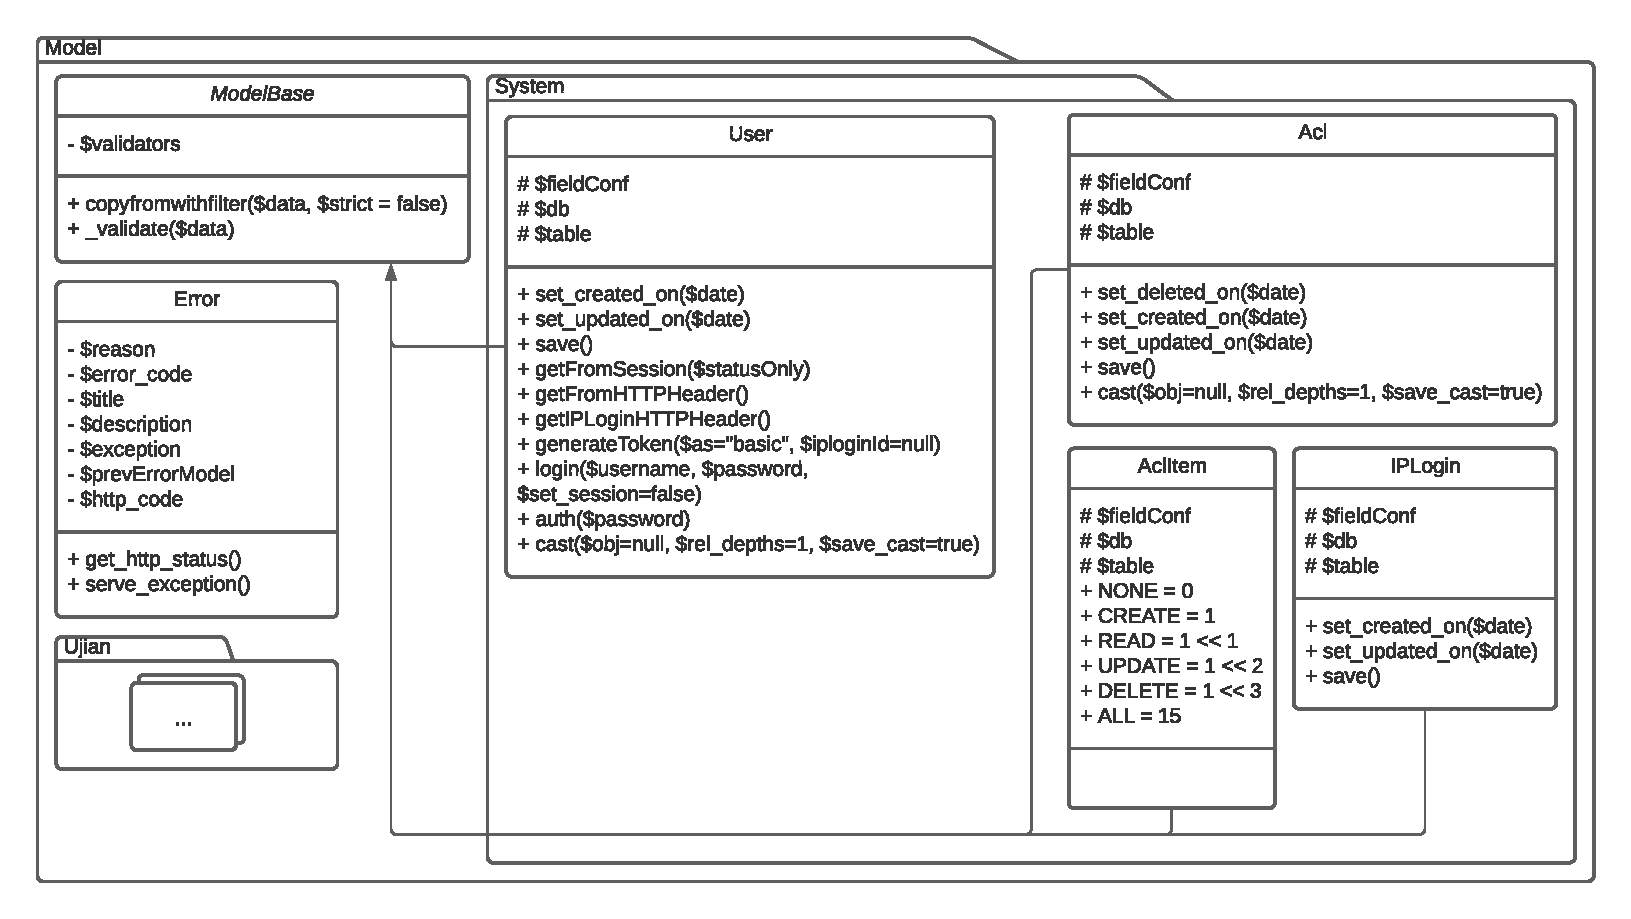
\includegraphics[width=0.8\paperheight]{Gambar/classmap-be/Classmap - app-model.pdf}
        \caption{Potongan diagram kelas untuk \textit{namespace}
        \texttt{Model}.}
        \label{fig:classmap_app-model}
    \end{sidewaysfigure}
    \textit{Namespace} ini akan berisi kelas-kelas yang bertanggung jawab
    merepresentasikan entitas dalam bentuk kelas dengan memanfaatkan teknologi
    ORM. Diagram kelas tersebut dapat dilihat pada Gambar
    \ref{fig:classmap_app-model}.
    
    Kelas-kelas yang terdapat pada \textit{namespace} ini terdiri dari
    \begin{itemize}
        \item \texttt{ModelBase} \\
            Kelas ini bertanggung jawab untuk menyediakan abstraksi untuk setiap
            model yang digunakan pada aplikasi. Atribut yang terdapat pada kelas
            ini adalah:
            \begin{itemize}
                \item \texttt{\$validators}: Digunakan untuk menyimpan daftar
                    validator dalam bentuk pasangan key-value, tergantung dari
                    jenis kolom yang didefinisikan pada kelas representasi
                    entitasnya.
            \end{itemize}
            Selain itu, fungsi yang dimiliki oleh kelas ini adalah:
            \begin{itemize}
                \item \texttt{copyfromwithfilter(\$data, \$strict = false))}\\
                    Bertanggung jawab untuk melakukan penyalinan data dengan
                    syarat yang terdapat pada definisi kelas representasi
                    entitas.\\
                    \textbf{Input:} Data yang ada, apakah harus berada dalam
                    mode ketat.\\
                    \textbf{Output:} -
                    
                \item \texttt{\_validate(\$data))}\\
                    Bertanggung jawab untuk melakukan validasi data yang
                    diberikan dengan tabel definisi validasi yang diberikan pada
                    atribut \$validator.\\
                    \textbf{Input:} data yang akan divalidasi\\
                    \textbf{Output:} \texttt{true} jika data valid,
                        \textit{Exception} jika terdapat pelangaran validasi.
            \end{itemize}
            
        \item \texttt{Error} \\
            Bertanggung jawab untuk memodelkan pesan kesalahan yang dapat
            diserialisasi menjadi respon yang dapat dipresentasikan untuk
            pengkonsumsi API. Kelas ini bukan bagian dari entitas ataupun ORM,
            kelas ini bagian dari sistem dan siklus hidupnya. Kelas ini memiliki
            atribut:
            \begin{itemize}
                \item \texttt{\$reason}: Menyimpan informasi alasan singkat
                    kenapa pesan kesalahan ini diterbitkan.
                \item \texttt{\$error\_code}: Menyimpan informasi kode kesalahan
                untuk internal sistem.
                \item \texttt{\$title}: Menyimpan informasi judul dari pesan
                kesalahan ini.
                \item \texttt{\$description}: Menyimpan informasi detil dari
                kesalahan yang muncul.
                \item \texttt{\$exception}: Objek eksepsi sebagai pendukung
                informasi pesan kesalahan.
                \item \texttt{\$prevErrorModel}: Objek kesalahan sebelumnya
                    sebagai pendukung informasi pesan kesalahan.
                \item \texttt{\$http\_code}: Kode HTTP yang dapat
                    merepresentasikan pesan kesalahan ini. (Contohnya 400 untuk
                    permintaan yang tidak valid, 500 untuk galat yang tidak
                    terduga, dan seterusnya).
            \end{itemize}
            Selain itu, kelas ini memiliki fungsi:
            \begin{itemize}
                \item \texttt{get\_http\_status()} \\
                    \textit{Getter} untuk kode respon HTTP pada pesan kesalahan
                    ini. \\
                    \textbf{Input:} - \\
                    \textbf{Output:} kode respon HTTP dalam representasi angka
                        maupun \textit{string}.
                    
                \item \texttt{serve\_exception()} \\
                    Bertanggung jawab untuk memformat pesan kesalahan sebelum
                    disajikan pada pengkonsumsi API. \\
                    \textbf{Input:} - \\
                    \textbf{Output:} representasi pesan kesalahan dalam bentuk
                        pasangan \textit{hashmap key-value}.
            \end{itemize}
                
        \item \texttt{System\textbackslash User} \\
            Kelas ini merepresentasikan entitas User, bagian dari ORM,
            bertanggung jawab untuk menerbitkan token untuk otentikasi, juga
            mendeteksi pengguna yang terotentikasi berdasarkan informasi header.
            Kelas ini memiliki atribut yang diturunkan dari kelas utama ORM,
            F3-Cortex. Atribut-atribut tersebut terdiri dari
            \begin{itemize}
                \item \texttt{\$fieldConf}\\
                    Digunakan untuk mendefinisikan kolom-kolom yang terdapat
                    pada tabel \textit{User}.
                \item \texttt{\$db} dengan nilai awal \texttt{"DB"}. \\
                    Menentukan database yang akan digunakan pada model ini.
                \item \texttt{\$table} dengan nilai awal
                \texttt{"system\_user"}. \\
                    Nama tabel yang akan digunakan pada sistem basis data. 
            \end{itemize}
            Sedangkan fungsi yang terdapat pada kelas ini adalah:
            \begin{itemize}
                \item \texttt{set\_created\_on(\$date)} \\
                    Mengkonversi bentuk tanggal kolom \texttt{created\_on}
                    \textit{native} ke format basis data. \\
                    \textbf{Input:} Tanggal dalam bentuk \textit{Unix time}\\
                    \textbf{Output:} \textit{string} tanggal terformat.
                
                \item \texttt{set\_updated\_on(\$date)} \\
                    Mengkonversi bentuk tanggal kolom \texttt{updated\_on}
                    \textit{native} ke format basis data. \\
                    \textbf{Input:} Tanggal dalam bentuk \textit{Unix time}\\
                    \textbf{Output:} \textit{string} tanggal terformat.
                
                \item \texttt{save()} \\
                    Meng-\textit{override} kelas dari ORM. Bertanggung jawab
                    untuk mengisi kolom \textit{created\_on} dan
                    \textit{updated\_on}.\\
                    \textbf{Input:} -\\
                    \textbf{Output:} -
                
                \item \texttt{getFromSession(\$statusOnly)} \\
                    Bertanggung jawab untuk menlakukan pengecekan pengguna
                    terotentikasi melalui \textit{session}. \\
                    \textbf{Input:} Apakah bentuk kembalian yang diinginkan
                        hanyalah statusnya saja atau objek penuh\\
                    \textbf{Output:} \texttt{null} pada saat kosong,
                        \texttt{"user"} atau objek dari kelas ini jika
                        otentikasi ditemukan.
                
                \item \texttt{getFromHTTPHeader()} \\
                    Cek otentikasi dari kepala permintaan HTTP. \\
                    \textbf{Input:} - \\
                    \textbf{Output:} Objek dari kelas ini jika terdapat
                        otentikasi, \texttt{false} jika tidak ada.
                
                \item \texttt{getIPLoginHTTPHeader()} \\
                    Cek IPLogin dari kepala permintaan HTTP pada otentikasi yang
                    terhubung. \\
                    \textbf{Input:} -\\
                    \textbf{Output:} Objek dari kelas \texttt{IPLogin} jika
                        terdapat otentikasi, \texttt{null} jika tidak ada.
                
                \item \texttt{generateToken(\$as="basic", \$iploginId=null)} \\
                    Bangkitkan token JWT untuk pengguna ini. \\
                    \textbf{Input:} Peran token ini, IPLogin tertaut.\\
                    \textbf{Output:} \textit{string} token.
                
                \item \texttt{login(\$username, \$password,
                \$set\_session=false)} \\
                    Lakukan pengecekkan kredensial login berdasarkan nama
                    pengguna dan password. \\
                    \textbf{Input:} nama pengguna, kata sandi, apakah ingin
                        sekaligus disimpan ke \textit{session}\\
                    \textbf{Output:} Objek dari user dimaksud, atau
                        \textit{Exception} jika terdapat kesalahan.
                
                \item \texttt{auth(\$password)} \\
                    Lakukan verifikasi kata sandi yang dimiliki pengguna ini. \\
                    \textbf{Input:} Kata sandi dari pengguna.\\
                    \textbf{Output:} \textit{boolean} apakah password benar atau
                    tidak.
                
                \item \texttt{cast(\$obj=null, \$rel\_depths=1,
                \$save\_cast=true)} \\
                    Meng-\textit{override} kelas dari ORM. Bertanggung jawab
                    untuk merepresentasikan kelas dalam bentuk \textit{hashmap}
                    secara aman atau tidak. \\
                    \textbf{Input:} Instansi yang akan di-\textit{cast},
                        konfigurasi relasi, dan lakukan \textit{casting} yang
                        aman atau tidak.\\
                    \textbf{Output:} \textit{array}.

            \end{itemize}
            
        \item \texttt{System\textbackslash Acl} \\
            Kelas ini merepresentasikan entitas \textit{Access Control List}
            atau ACL. Kelas ini bagian dari ORM. Atribut yang terdapat pada
            kelas ini terdiri dari:
            \begin{itemize}
                \item \texttt{\$fieldConf} \\
                    Digunakan untuk mendefinisikan kolom-kolom yang terdapat
                    pada tabel \textit{ACL}.
                \item \texttt{\$db} dengan nilai awal \texttt{"DB"}. \\
                    Menentukan database yang akan digunakan pada model ini.
                \item \texttt{\$table} dengan nilai awal \texttt{"system\_acl"}.
                \\
                    Nama tabel yang akan digunakan pada sistem basis data. 
            \end{itemize}
            Sedangkan fungsi yang terdapat pada kelas ini adalah:
            \begin{itemize}
                \item \texttt{set\_deleted\_on(\$date)}\\
                    Mengkonversi bentuk tanggal kolom \texttt{deleted\_on}
                    \textit{native} ke format basis data. \\
                    \textbf{Input:} Tanggal dalam bentuk \textit{Unix time}\\
                    \textbf{Output:} \textit{string} tanggal terformat.
                
                \item \texttt{set\_created\_on(\$date)} \\
                    Mengkonversi bentuk tanggal kolom \texttt{created\_on}
                    \textit{native} ke format basis data. \\
                    \textbf{Input:} Tanggal dalam bentuk \textit{Unix time}\\
                    \textbf{Output:} \textit{string} tanggal terformat.
                
                \item \texttt{set\_updated\_on(\$date)} \\
                    Mengkonversi bentuk tanggal kolom \texttt{updated\_on}
                    \textit{native} ke format basis data. \\
                    \textbf{Input:} Tanggal dalam bentuk \textit{Unix time}\\
                    \textbf{Output:} \textit{string} tanggal terformat.
                
                \item \texttt{save()}\\
                    Meng-\textit{override} kelas dari ORM. Bertanggung jawab
                    untuk mengisi kolom \textit{created\_on} dan
                    \textit{updated\_on}.\\
                    \textbf{Input:} -\\
                    \textbf{Output:} -
                
                \item \texttt{cast(\$obj=null, \$rel\_depths=1,
                \$save\_cast=true)}\\
                    Meng-\textit{override} kelas dari ORM. Bertanggung jawab
                    untuk merepresentasikan kelas dalam bentuk \textit{hashmap}
                    secara aman atau tidak. \\
                    \textbf{Input:} Instansi yang akan di-\textit{cast},
                        konfigurasi relasi, dan lakukan \textit{casting} yang
                        aman atau tidak.\\
                    \textbf{Output:} \textit{array}.
            \end{itemize}
            
        \item \texttt{System\textbackslash AclItem} \\
            Kelas ini adalah kelas terkait ORM yang merepresentasikan entitas
            AclItem. Kelas ini memiliki daftar atribut:
            \begin{itemize}
                \item \texttt{\$fieldConf} \\
                    Digunakan untuk mendefinisikan kolom-kolom yang terdapat
                    pada tabel \textit{ACLItem}.
                \item \texttt{\$db} dengan nilai awal \texttt{"DB"}. \\
                    Menentukan database yang akan digunakan pada model ini.
                \item \texttt{\$table} dengan nilai awal
                \texttt{"system\_aclitem"}. \\
                    Nama tabel yang akan digunakan pada sistem basis data. 
                \item \texttt{NONE}: Nilai konstanta tidak memiliki izin apapun.
                \item \texttt{CREATE}: Nilai konstanta untuk izin membuat.
                \item \texttt{READ}: Nilai konstanta untuk izin membaca/melihat.
                \item \texttt{UPDATE}: Nilai konstanta untuk izin
                mengubah/memperbarui.
                \item \texttt{DELETE}: Nilai konstanta untuk izin menghapus.
                \item \texttt{ALL}: Nilai konstanta untuk semua izin
                diperbolehkan.
            \end{itemize}
            
        \item \texttt{System\textbackslash IPLogin} \\
            Kelas ini adalah kelas terkait ORM yang merepresentasikan entitas
            IPlogin. Atribut yang terdapat pada kelas ini terdiri dari:
            \begin{itemize}
                \item \texttt{\$fieldConf} \\
                    Digunakan untuk mendefinisikan kolom-kolom yang terdapat
                    pada tabel \textit{ACL}.
                \item \texttt{\$db} dengan nilai awal \texttt{"DB"}. \\
                    Menentukan database yang akan digunakan pada model ini.
                \item \texttt{\$table} dengan nilai awal
                \texttt{"system\_iplogin"}. \\
                    Nama tabel yang akan digunakan pada sistem basis data. 
            \end{itemize}
            Sedangkan fungsi yang terdapat pada kelas ini adalah:
            \begin{itemize}
                \item \texttt{set\_created\_on(\$date)} \\
                    Mengkonversi bentuk tanggal kolom \texttt{created\_on}
                    \textit{native} ke format basis data. \\
                    \textbf{Input:} Tanggal dalam bentuk \textit{Unix time}\\
                    \textbf{Output:} \textit{string} tanggal terformat.
                
                \item \texttt{set\_updated\_on(\$date)} \\
                    Mengkonversi bentuk tanggal kolom \texttt{updated\_on}
                    \textit{native} ke format basis data. \\
                    \textbf{Input:} Tanggal dalam bentuk \textit{Unix time}\\
                    \textbf{Output:} \textit{string} tanggal terformat.
                
                \item \texttt{save()}\\
                    Meng-\textit{override} kelas dari ORM. Bertanggung jawab
                    untuk mengisi kolom \textit{created\_on} dan
                    \textit{updated\_on}.\\
                    \textbf{Input:} -\\
                    \textbf{Output:} -
            \end{itemize}
    \end{itemize}
    
    
    \begin{sidewaysfigure}
        \centering
        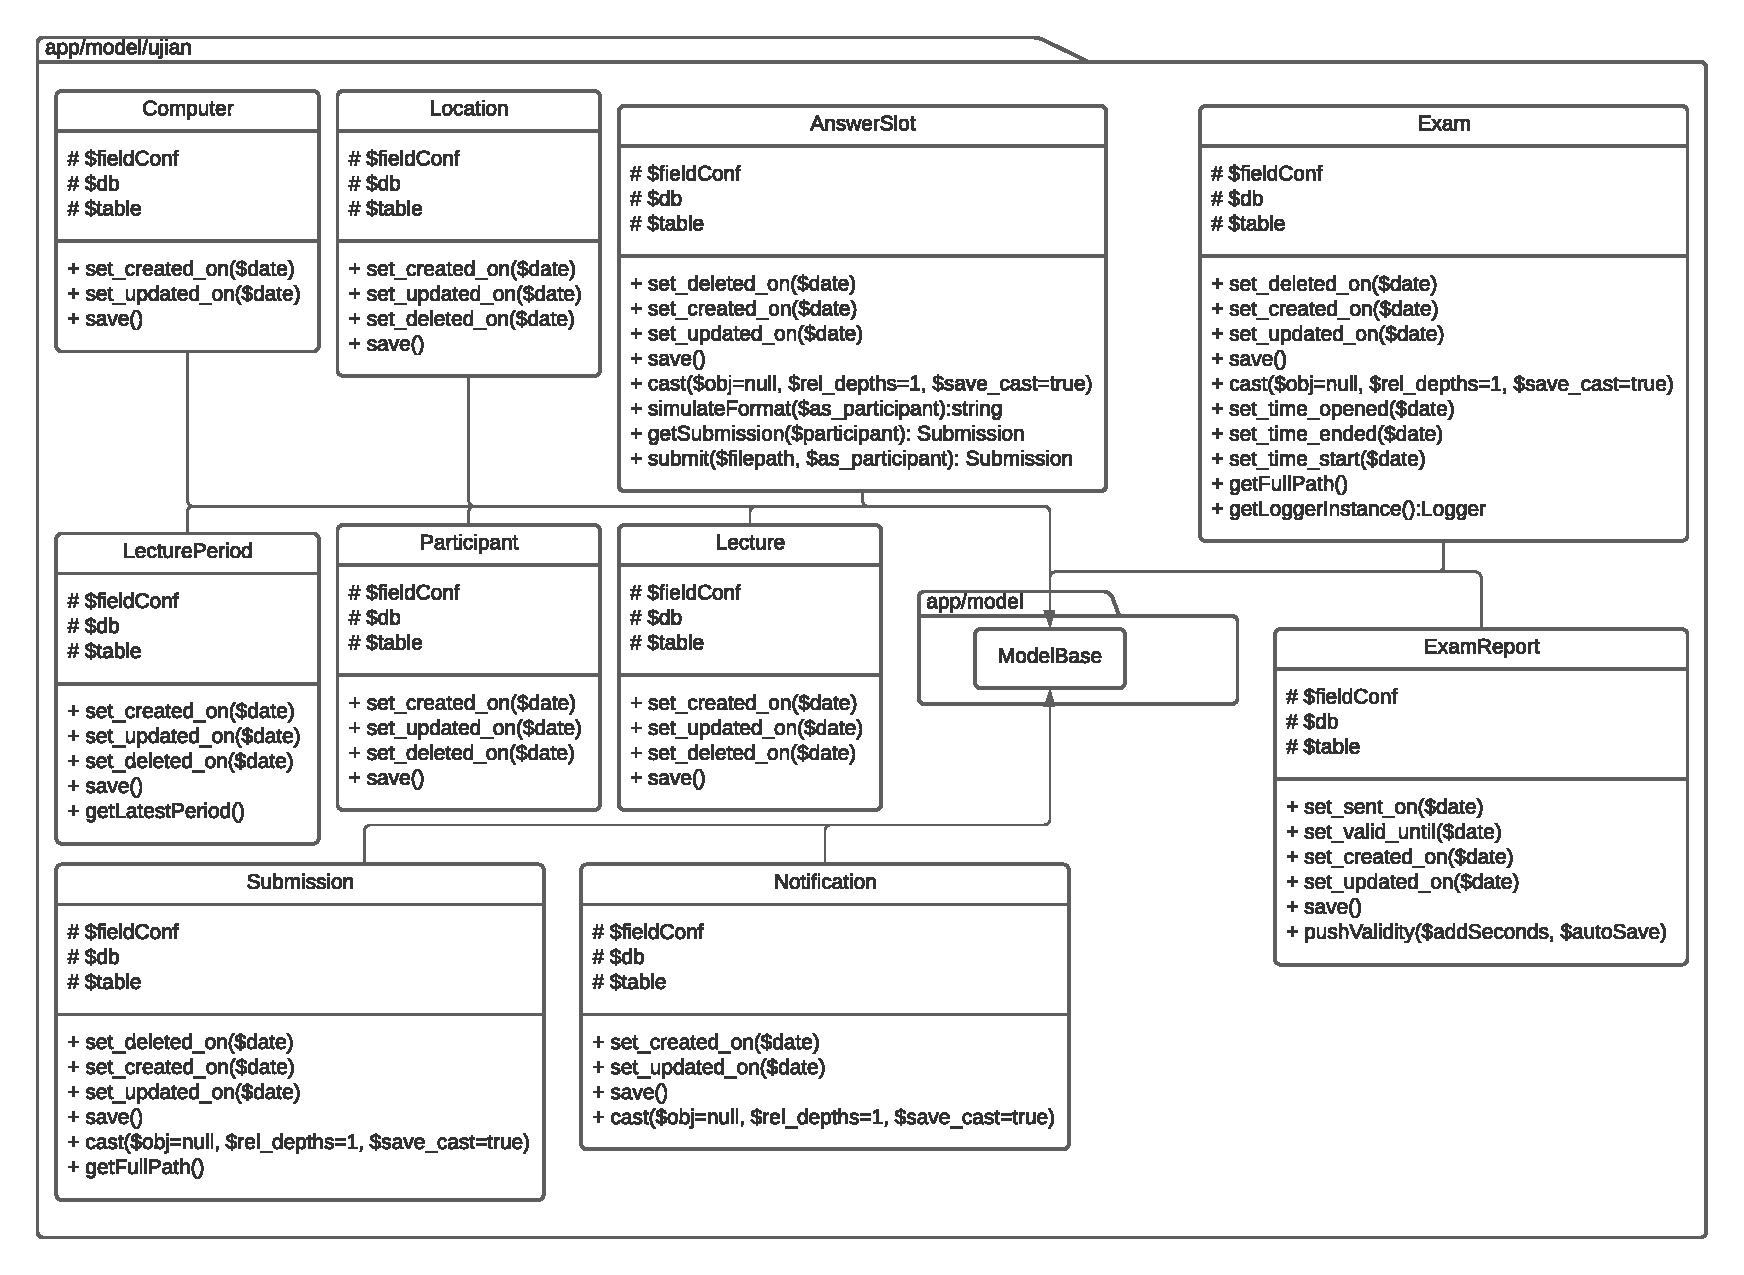
\includegraphics[width=0.8\paperheight]{Gambar/classmap-be/Classmap - app-model-ujian.pdf}
        \caption{Potongan diagram kelas untuk \textit{namespace}
        \texttt{Model/ujian}.}
        \label{fig:classmap_app-model-ujian}
    \end{sidewaysfigure}
    \textit{Namespace} \texttt{Model\textbackslash Ujian} memiliki beberapa
    kelas ORM yang berhubungan langsung dengan ujian. Diagram kelas untuk
    \textit{namespace} tersebut dapat dilihat pada Gambar
    \ref{fig:classmap_app-model-ujian}. Kelas-kelas pada \textit{namespace} ini
    terdiri dari
    \begin{itemize}
        \item \texttt{Computer} \\
            Kelas ini adalah kelas terkait ORM yang merepresentasikan entitas
            Computer. Atribut yang terdapat pada kelas ini terdiri dari:
            \begin{itemize}
                \item \texttt{\$fieldConf} \\
                    Digunakan untuk mendefinisikan kolom-kolom yang terdapat
                    pada tabel \textit{Computer}.
                \item \texttt{\$db} dengan nilai awal \texttt{"DB"}. \\
                    Menentukan database yang akan digunakan pada model ini.
                \item \texttt{\$table} dengan nilai awal
                \texttt{"ujian\_computer"}. \\
                    Nama tabel yang akan digunakan pada sistem basis data. 
            \end{itemize}
            Sedangkan fungsi yang terdapat pada kelas ini adalah:
            \begin{itemize}
                \item \texttt{set\_created\_on(\$date)} \\
                    Mengkonversi bentuk tanggal kolom \texttt{created\_on}
                    \textit{native} ke format basis data. \\
                    \textbf{Input:} Tanggal dalam bentuk \textit{Unix time}\\
                    \textbf{Output:} \textit{string} tanggal terformat.
                
                \item \texttt{set\_updated\_on(\$date)} \\
                    Mengkonversi bentuk tanggal kolom \texttt{updated\_on}
                    \textit{native} ke format basis data. \\
                    \textbf{Input:} Tanggal dalam bentuk \textit{Unix time}\\
                    \textbf{Output:} \textit{string} tanggal terformat.
                
                \item \texttt{save()}\\
                    Meng-\textit{override} kelas dari ORM. Bertanggung jawab
                    untuk mengisi kolom \textit{created\_on} dan
                    \textit{updated\_on}.\\
                    \textbf{Input:} -\\
                    \textbf{Output:} -
            \end{itemize}
            
        \item \texttt{Location} \\
            Kelas ini adalah kelas terkait ORM yang merepresentasikan entitas
            Location. Atribut yang terdapat pada kelas ini terdiri dari:
            \begin{itemize}
                \item \texttt{\$fieldConf} \\
                    Digunakan untuk mendefinisikan kolom-kolom yang terdapat
                    pada tabel \textit{Location}.
                \item \texttt{\$db} dengan nilai awal \texttt{"DB"}. \\
                    Menentukan database yang akan digunakan pada model ini.
                \item \texttt{\$table} dengan nilai awal
                \texttt{"ujian-computer"}. \\
                    Nama tabel yang akan digunakan pada sistem basis data. 
            \end{itemize}
            Sedangkan fungsi yang terdapat pada kelas ini adalah:
            \begin{itemize}
                \item \texttt{set\_created\_on(\$date)} \\
                    Mengkonversi bentuk tanggal kolom \texttt{created\_on}
                    \textit{native} ke format basis data. \\
                    \textbf{Input:} Tanggal dalam bentuk \textit{Unix time}\\
                    \textbf{Output:} \textit{string} tanggal terformat.
                
                \item \texttt{set\_updated\_on(\$date)} \\
                    Mengkonversi bentuk tanggal kolom \texttt{updated\_on}
                    \textit{native} ke format basis data. \\
                    \textbf{Input:} Tanggal dalam bentuk \textit{Unix time}\\
                    \textbf{Output:} \textit{string} tanggal terformat.
                    
                \item \texttt{set\_deleted\_on(\$date)} \\
                    Mengkonversi bentuk tanggal kolom \texttt{deleted\_on}
                    \textit{native} ke format basis data. \\
                    \textbf{Input:} Tanggal dalam bentuk \textit{Unix time}\\
                    \textbf{Output:} \textit{string} tanggal terformat.
                    
                \item \texttt{save()}\\
                    Meng-\textit{override} kelas dari ORM. Bertanggung jawab
                    untuk mengisi kolom \textit{created\_on},
                    \textit{updated\_on} dan \textit{deleted\_on}.\\
                    \textbf{Input:} -\\
                    \textbf{Output:} -
            \end{itemize}
            
        \item \texttt{AnswerSlot} \\
            Kelas ini adalah kelas terkait ORM yang merepresentasikan entitas
            AnswerSlot. Atribut yang terdapat pada kelas ini terdiri dari:
            \begin{itemize}
                \item \texttt{\$fieldConf} \\
                    Digunakan untuk mendefinisikan kolom-kolom yang terdapat
                    pada tabel \textit{AnswerSlot}.
                \item \texttt{\$db} dengan nilai awal \texttt{"DB"}. \\
                    Menentukan database yang akan digunakan pada model ini.
                \item \texttt{\$table} dengan nilai awal
                \texttt{"ujian-computer"}. \\
                    Nama tabel yang akan digunakan pada sistem basis data. 
            \end{itemize}
            Sedangkan fungsi yang terdapat pada kelas ini adalah:
            \begin{itemize}
                \item \texttt{set\_created\_on(\$date)} \\
                    Mengkonversi bentuk tanggal kolom \texttt{created\_on}
                    \textit{native} ke format basis data. \\
                    \textbf{Input:} Tanggal dalam bentuk \textit{Unix time}\\
                    \textbf{Output:} \textit{string} tanggal terformat.
                
                \item \texttt{set\_updated\_on(\$date)} \\
                    Mengkonversi bentuk tanggal kolom \texttt{updated\_on}
                    \textit{native} ke format basis data. \\
                    \textbf{Input:} Tanggal dalam bentuk \textit{Unix time}\\
                    \textbf{Output:} \textit{string} tanggal terformat.
                    
                \item \texttt{set\_deleted\_on(\$date)} \\
                    Mengkonversi bentuk tanggal kolom \texttt{deleted\_on}
                    \textit{native} ke format basis data. \\
                    \textbf{Input:} Tanggal dalam bentuk \textit{Unix time}\\
                    \textbf{Output:} \textit{string} tanggal terformat.
                    
                \item \texttt{save()}\\
                    Meng-\textit{override} kelas dari ORM. Bertanggung jawab
                    untuk mengisi kolom \textit{created\_on},
                    \textit{updated\_on} dan \textit{deleted\_on}.\\
                    \textbf{Input:} -\\
                    \textbf{Output:} -
                
                \item \texttt{cast(\$obj=null, \$rel\_depths=1,
                \$save\_cast=true)}\\
                    Meng-\textit{override} kelas dari ORM. Bertanggung jawab
                    untuk merepresentasikan kelas dalam bentuk \textit{hashmap}
                    secara aman atau tidak. \\
                    \textbf{Input:} Instansi yang akan di-\textit{cast},
                        konfigurasi relasi, dan lakukan \textit{casting} yang
                        aman atau tidak.\\
                    \textbf{Output:} \textit{array}.
                    
                \item \texttt{simulateFormat(\$as\_participant)} \\
                    Bertanggung jawab untuk membangkitkan nama berkas yang
                    ditunjukkan untuk slot jawaban ini pada peserta tertentu. \\
                    \textbf{Input:} Detil peserta dalam kelas
                    \texttt{Participant}.\\
                    \textbf{Output:} \textit{string} nama berkas jawaban.
                    
                \item \texttt{getSubmission(\$participant)} \\
                    Bertanggung jawab untuk mengembalikan instansi
                    \texttt{Submission} untuk peserta tertentu. \\
                    \textbf{Input:} Instansi objek peserta.\\
                    \textbf{Output:} objek \texttt{Submission}
                    
                \item \texttt{submit(\$filepath, \$as\_participant)} \\
                    Melakukan submisi untuk slot jawaban ini dengan informasi
                    lokasi berkas dan informasi peserta. \\
                    \textbf{Input:} Lokasi berkas, objek \texttt{Participant}.\\
                    \textbf{Output:} objek \texttt{Submission}
                    
            \end{itemize}
            
        \item \texttt{Exam} \\
            Kelas ini adalah kelas terkait ORM yang merepresentasikan entitas
            Exam. Atribut yang terdapat pada kelas ini terdiri dari:
            \begin{itemize}
                \item \texttt{\$fieldConf} \\
                    Digunakan untuk mendefinisikan kolom-kolom yang terdapat
                    pada tabel \textit{Exam}.
                \item \texttt{\$db} dengan nilai awal \texttt{"DB"}. \\
                    Menentukan database yang akan digunakan pada model ini.
                \item \texttt{\$table} dengan nilai awal \texttt{"ujian-exam"}.
                \\
                    Nama tabel yang akan digunakan pada sistem basis data. 
            \end{itemize}
            Sedangkan fungsi yang terdapat pada kelas ini adalah:
            \begin{itemize}
                \item \texttt{set\_created\_on(\$date)} \\
                    Mengkonversi bentuk tanggal kolom \texttt{created\_on}
                    \textit{native} ke format basis data. \\
                    \textbf{Input:} Tanggal dalam bentuk \textit{Unix time}\\
                    \textbf{Output:} \textit{string} tanggal terformat.
                
                \item \texttt{set\_updated\_on(\$date)} \\
                    Mengkonversi bentuk tanggal kolom \texttt{updated\_on}
                    \textit{native} ke format basis data. \\
                    \textbf{Input:} Tanggal dalam bentuk \textit{Unix time}\\
                    \textbf{Output:} \textit{string} tanggal terformat.
                    
                \item \texttt{set\_deleted\_on(\$date)} \\
                    Mengkonversi bentuk tanggal kolom \texttt{deleted\_on}
                    \textit{native} ke format basis data. \\
                    \textbf{Input:} Tanggal dalam bentuk \textit{Unix time}\\
                    \textbf{Output:} \textit{string} tanggal terformat.
                    
                \item \texttt{save()}\\
                    Meng-\textit{override} kelas dari ORM. Bertanggung jawab
                    untuk mengisi kolom \textit{created\_on},
                    \textit{updated\_on} dan \textit{deleted\_on}.\\
                    \textbf{Input:} -\\
                    \textbf{Output:} -
                
                \item \texttt{cast(\$obj=null, \$rel\_depths=1,
                \$save\_cast=true)}\\
                    Meng-\textit{override} kelas dari ORM. Bertanggung jawab
                    untuk merepresentasikan kelas dalam bentuk \textit{hashmap}
                    secara aman atau tidak. \\
                    \textbf{Input:} Instansi yang akan di-\textit{cast},
                        konfigurasi relasi, dan lakukan \textit{casting} yang
                        aman atau tidak.\\
                    \textbf{Output:} \textit{array}.
                    
                \item \texttt{set\_time\_opened(\$date)} \\
                     Mengkonversi bentuk tanggal kolom \texttt{time\_opened}
                    \textit{native} ke format basis data. \\
                    \textbf{Input:} Tanggal dalam bentuk \textit{Unix time}\\
                    \textbf{Output:} \textit{string} tanggal terformat.
                
                \item \texttt{set\_time\_ended(\$date)} \\
                    Mengkonversi bentuk tanggal kolom \texttt{time\_ended}
                    \textit{native} ke format basis data. \\
                    \textbf{Input:} Tanggal dalam bentuk \textit{Unix time}\\
                    \textbf{Output:} \textit{string} tanggal terformat.
                
                \item \texttt{set\_time\_start(\$date)} \\
                    Mengkonversi bentuk tanggal kolom \texttt{time\_start}
                    \textit{native} ke format basis data. \\
                    \textbf{Input:} Tanggal dalam bentuk \textit{Unix time}\\
                    \textbf{Output:} \textit{string} tanggal terformat.
                
                \item \texttt{getFullPath()} \\
                    Bertanggung jawab untuk mengembalikan alamat lengkap dari
                    ujian ini. \\
                    \textbf{Input:} -\\
                    \textbf{Output:} \textit{string} alamat lengkap menuju
                    folder ujian ini.
                
                \item \texttt{getLoggerInstance(\$loggerName = "general")} \\
                    Bertanggung jawab untuk mengembalikan objek \texttt{Logger}
                    yang dapat digunakan untuk melakukan logging\\
                    \textbf{Input:} Nama label untuk log yang ingin dibuat\\
                    \textbf{Output:} Objek \texttt{Logger}
            \end{itemize}
            
        \item \texttt{LecturePeriod} \\
            Kelas ini adalah kelas terkait ORM yang merepresentasikan entitas
            LecturePeriod. Atribut yang terdapat pada kelas ini terdiri dari:
            \begin{itemize}
                \item \texttt{\$fieldConf} \\
                    Digunakan untuk mendefinisikan kolom-kolom yang terdapat
                    pada tabel \textit{LecturePeriod}.
                \item \texttt{\$db} dengan nilai awal \texttt{"DB"}. \\
                    Menentukan database yang akan digunakan pada model ini.
                \item \texttt{\$table} dengan nilai awal
                \texttt{"ujian\_computer"}. \\
                    Nama tabel yang akan digunakan pada sistem basis data. 
            \end{itemize}
            Sedangkan fungsi yang terdapat pada kelas ini adalah:
            \begin{itemize}
                \item \texttt{set\_created\_on(\$date)} \\
                    Mengkonversi bentuk tanggal kolom \texttt{created\_on}
                    \textit{native} ke format basis data. \\
                    \textbf{Input:} Tanggal dalam bentuk \textit{Unix time}\\
                    \textbf{Output:} \textit{string} tanggal terformat.
                
                \item \texttt{set\_updated\_on(\$date)} \\
                    Mengkonversi bentuk tanggal kolom \texttt{updated\_on}
                    \textit{native} ke format basis data. \\
                    \textbf{Input:} Tanggal dalam bentuk \textit{Unix time}\\
                    \textbf{Output:} \textit{string} tanggal terformat.
                    
                \item \texttt{set\_deleted\_on(\$date)} \\
                    Mengkonversi bentuk tanggal kolom \texttt{deleted\_on}
                    \textit{native} ke format basis data. \\
                    \textbf{Input:} Tanggal dalam bentuk \textit{Unix time}\\
                    \textbf{Output:} \textit{string} tanggal terformat.
                    
                \item \texttt{save()}\\
                    Meng-\textit{override} kelas dari ORM. Bertanggung jawab
                    untuk mengisi kolom \textit{created\_on},
                    \textit{updated\_on} dan \textit{deleted\_on}.\\
                    \textbf{Input:} -\\
                    \textbf{Output:} -
                    
                \item \texttt{getLatestPeriod()}\\
                    Bertanggung jawab untuk mengambil periode terbaru pada tahun
                    aktif. Jika tidak tersedia pada basis data, maka fungsi ini
                    akan membuat periode yang baru.\\
                    \textbf{Input:} -\\
                    \textbf{Output:} Objek \textit{LecturePeriod} berisi baris
                    tertentu.
            \end{itemize}
            
        \item \texttt{Participant} \\
            Kelas ini adalah kelas terkait ORM yang merepresentasikan entitas
            Participant. Atribut yang terdapat pada kelas ini terdiri dari:
            \begin{itemize}
                \item \texttt{\$fieldConf} \\
                    Digunakan untuk mendefinisikan kolom-kolom yang terdapat
                    pada tabel \textit{Participant}.
                \item \texttt{\$db} dengan nilai awal \texttt{"DB"}. \\
                    Menentukan database yang akan digunakan pada model ini.
                \item \texttt{\$table} dengan nilai awal
                \texttt{"ujian\_participant"}. \\
                    Nama tabel yang akan digunakan pada sistem basis data. 
            \end{itemize}
            Sedangkan fungsi yang terdapat pada kelas ini adalah:
            \begin{itemize}
                \item \texttt{set\_created\_on(\$date)} \\
                    Mengkonversi bentuk tanggal kolom \texttt{created\_on}
                    \textit{native} ke format basis data. \\
                    \textbf{Input:} Tanggal dalam bentuk \textit{Unix time}\\
                    \textbf{Output:} \textit{string} tanggal terformat.
                
                \item \texttt{set\_updated\_on(\$date)} \\
                    Mengkonversi bentuk tanggal kolom \texttt{updated\_on}
                    \textit{native} ke format basis data. \\
                    \textbf{Input:} Tanggal dalam bentuk \textit{Unix time}\\
                    \textbf{Output:} \textit{string} tanggal terformat.
                    
                \item \texttt{set\_deleted\_on(\$date)} \\
                    Mengkonversi bentuk tanggal kolom \texttt{deleted\_on}
                    \textit{native} ke format basis data. \\
                    \textbf{Input:} Tanggal dalam bentuk \textit{Unix time}\\
                    \textbf{Output:} \textit{string} tanggal terformat.
                    
                \item \texttt{save()}\\
                    Meng-\textit{override} kelas dari ORM. Bertanggung jawab
                    untuk mengisi kolom \textit{created\_on},
                    \textit{updated\_on} dan \textit{deleted\_on}.\\
                    \textbf{Input:} -\\
                    \textbf{Output:} -
            \end{itemize}
            
        \item \texttt{Lecture} \\
            Kelas ini adalah kelas terkait ORM yang merepresentasikan entitas
            Lecture. Atribut yang terdapat pada kelas ini terdiri dari:
            \begin{itemize}
                \item \texttt{\$fieldConf} \\
                    Digunakan untuk mendefinisikan kolom-kolom yang terdapat
                    pada tabel \textit{Lecture}.
                \item \texttt{\$db} dengan nilai awal \texttt{"DB"}. \\
                    Menentukan database yang akan digunakan pada model ini.
                \item \texttt{\$table} dengan nilai awal
                \texttt{"ujian\_lecture"}. \\
                    Nama tabel yang akan digunakan pada sistem basis data. 
            \end{itemize}
            Sedangkan fungsi yang terdapat pada kelas ini adalah:
            \begin{itemize}
                \item \texttt{set\_created\_on(\$date)} \\
                    Mengkonversi bentuk tanggal kolom \texttt{created\_on}
                    \textit{native} ke format basis data. \\
                    \textbf{Input:} Tanggal dalam bentuk \textit{Unix time}\\
                    \textbf{Output:} \textit{string} tanggal terformat.
                
                \item \texttt{set\_updated\_on(\$date)} \\
                    Mengkonversi bentuk tanggal kolom \texttt{updated\_on}
                    \textit{native} ke format basis data. \\
                    \textbf{Input:} Tanggal dalam bentuk \textit{Unix time}\\
                    \textbf{Output:} \textit{string} tanggal terformat.
                    
                \item \texttt{set\_deleted\_on(\$date)} \\
                    Mengkonversi bentuk tanggal kolom \texttt{deleted\_on}
                    \textit{native} ke format basis data. \\
                    \textbf{Input:} Tanggal dalam bentuk \textit{Unix time}\\
                    \textbf{Output:} \textit{string} tanggal terformat.
                    
                \item \texttt{save()}\\
                    Meng-\textit{override} kelas dari ORM. Bertanggung jawab
                    untuk mengisi kolom \textit{created\_on},
                    \textit{updated\_on} dan \textit{deleted\_on}.\\
                    \textbf{Input:} -\\
                    \textbf{Output:} -
            \end{itemize}
            
        \item \texttt{Submission} \\
            Kelas ini adalah kelas terkait ORM yang merepresentasikan entitas
            Submission. Atribut yang terdapat pada kelas ini terdiri dari:
            \begin{itemize}
                \item \texttt{\$fieldConf} \\
                    Digunakan untuk mendefinisikan kolom-kolom yang terdapat
                    pada tabel \textit{Submission}.
                \item \texttt{\$db} dengan nilai awal \texttt{"DB"}. \\
                    Menentukan database yang akan digunakan pada model ini.
                \item \texttt{\$table} dengan nilai awal
                \texttt{"ujian\_submission"}. \\
                    Nama tabel yang akan digunakan pada sistem basis data. 
            \end{itemize}
            Sedangkan fungsi yang terdapat pada kelas ini adalah:
            \begin{itemize}
                \item \texttt{set\_created\_on(\$date)} \\
                    Mengkonversi bentuk tanggal kolom \texttt{created\_on}
                    \textit{native} ke format basis data. \\
                    \textbf{Input:} Tanggal dalam bentuk \textit{Unix time}\\
                    \textbf{Output:} \textit{string} tanggal terformat.
                
                \item \texttt{set\_updated\_on(\$date)} \\
                    Mengkonversi bentuk tanggal kolom \texttt{updated\_on}
                    \textit{native} ke format basis data. \\
                    \textbf{Input:} Tanggal dalam bentuk \textit{Unix time}\\
                    \textbf{Output:} \textit{string} tanggal terformat.
                    
                \item \texttt{set\_deleted\_on(\$date)} \\
                    Mengkonversi bentuk tanggal kolom \texttt{deleted\_on}
                    \textit{native} ke format basis data. \\
                    \textbf{Input:} Tanggal dalam bentuk \textit{Unix time}\\
                    \textbf{Output:} \textit{string} tanggal terformat.
                    
                \item \texttt{save()}\\
                    Meng-\textit{override} kelas dari ORM. Bertanggung jawab
                    untuk mengisi kolom \textit{created\_on},
                    \textit{updated\_on} dan \textit{deleted\_on}.\\
                    \textbf{Input:} -\\
                    \textbf{Output:} -
                
                \item \texttt{cast(\$obj=null, \$rel\_depths=1,
                \$save\_cast=true)}\\
                    Meng-\textit{override} kelas dari ORM. Bertanggung jawab
                    untuk merepresentasikan kelas dalam bentuk \textit{hashmap}
                    secara aman atau tidak. \\
                    \textbf{Input:} Instansi yang akan di-\textit{cast},
                        konfigurasi relasi, dan lakukan \textit{casting} yang
                        aman atau tidak.\\
                    \textbf{Output:} \textit{array}.
                
                \item \texttt{getFullPath()} \\
                    Bertanggung jawab untuk mengembalikan alamat lengkap menuju
                    berkas submisi ini. \\
                    \textbf{Input:} -\\
                    \textbf{Output:} \textit{string} alamat lengkap menuju
                    berkas submisi
            \end{itemize}
            
        \item \texttt{Notification} \\
            Kelas ini adalah kelas terkait ORM yang merepresentasikan entitas
            Notification. Atribut yang terdapat pada kelas ini terdiri dari:
            \begin{itemize}
                \item \texttt{\$fieldConf} \\
                    Digunakan untuk mendefinisikan kolom-kolom yang terdapat
                    pada tabel \textit{Notification}.
                \item \texttt{\$db} dengan nilai awal \texttt{"DB"}. \\
                    Menentukan database yang akan digunakan pada model ini.
                \item \texttt{\$table} dengan nilai awal
                \texttt{"ujian\_notification"}. \\
                    Nama tabel yang akan digunakan pada sistem basis data. 
            \end{itemize}
            Sedangkan fungsi yang terdapat pada kelas ini adalah:
            \begin{itemize}
                \item \texttt{set\_created\_on(\$date)} \\
                    Mengkonversi bentuk tanggal kolom \texttt{created\_on}
                    \textit{native} ke format basis data. \\
                    \textbf{Input:} Tanggal dalam bentuk \textit{Unix time}\\
                    \textbf{Output:} \textit{string} tanggal terformat.
                
                \item \texttt{set\_updated\_on(\$date)} \\
                    Mengkonversi bentuk tanggal kolom \texttt{updated\_on}
                    \textit{native} ke format basis data. \\
                    \textbf{Input:} Tanggal dalam bentuk \textit{Unix time}\\
                    \textbf{Output:} \textit{string} tanggal terformat.
                    
                \item \texttt{set\_deleted\_on(\$date)} \\
                    Mengkonversi bentuk tanggal kolom \texttt{deleted\_on}
                    \textit{native} ke format basis data. \\
                    \textbf{Input:} Tanggal dalam bentuk \textit{Unix time}\\
                    \textbf{Output:} \textit{string} tanggal terformat.
                    
                \item \texttt{save()}\\
                    Meng-\textit{override} kelas dari ORM. Bertanggung jawab
                    untuk mengisi kolom \textit{created\_on},
                    \textit{updated\_on} dan \textit{deleted\_on}.\\
                    \textbf{Input:} -\\
                    \textbf{Output:} -
                
                \item \texttt{cast(\$obj=null, \$rel\_depths=1,
                \$save\_cast=true)}\\
                    Meng-\textit{override} kelas dari ORM. Bertanggung jawab
                    untuk merepresentasikan kelas dalam bentuk \textit{hashmap}
                    secara aman atau tidak. \\
                    \textbf{Input:} Instansi yang akan di-\textit{cast},
                        konfigurasi relasi, dan lakukan \textit{casting} yang
                        aman atau tidak.\\
                    \textbf{Output:} \textit{array}.
            \end{itemize}
            
        \item \texttt{ExamReport} \\
            Kelas ini adalah kelas terkait ORM yang merepresentasikan entitas
            ExamReport. Atribut yang terdapat pada kelas ini terdiri dari:
            \begin{itemize}
                \item \texttt{\$fieldConf} \\
                    Digunakan untuk mendefinisikan kolom-kolom yang terdapat
                    pada tabel \textit{ExamReport}.
                \item \texttt{\$db} dengan nilai awal \texttt{"DB"}. \\
                    Menentukan database yang akan digunakan pada model ini.
                \item \texttt{\$table} dengan nilai awal
                \texttt{"ujian\_examreport"}. \\
                    Nama tabel yang akan digunakan pada sistem basis data. 
            \end{itemize}
            Sedangkan fungsi yang terdapat pada kelas ini adalah:
            \begin{itemize}
                \item \texttt{set\_sent\_on(\$date)} \\
                    Mengkonversi bentuk tanggal kolom \texttt{sent\_on}
                    \textit{native} ke format basis data. \\
                    \textbf{Input:} Tanggal dalam bentuk \textit{Unix time}\\
                    \textbf{Output:} \textit{string} tanggal terformat.
                    
                \item \texttt{set\_valid\_untill(\$date)} \\
                    Mengkonversi bentuk tanggal kolom \texttt{valid\_untill}
                    \textit{native} ke format basis data. \\
                    \textbf{Input:} Tanggal dalam bentuk \textit{Unix time}\\
                    \textbf{Output:} \textit{string} tanggal terformat.
                    
                \item \texttt{set\_created\_on(\$date)} \\
                    Mengkonversi bentuk tanggal kolom \texttt{created\_on}
                    \textit{native} ke format basis data. \\
                    \textbf{Input:} Tanggal dalam bentuk \textit{Unix time}\\
                    \textbf{Output:} \textit{string} tanggal terformat.
                
                \item \texttt{set\_updated\_on(\$date)} \\
                    Mengkonversi bentuk tanggal kolom \texttt{updated\_on}
                    \textit{native} ke format basis data. \\
                    \textbf{Input:} Tanggal dalam bentuk \textit{Unix time}\\
                    \textbf{Output:} \textit{string} tanggal terformat.
                    
                    
                \item \texttt{save()}\\
                    Meng-\textit{override} kelas dari ORM. Bertanggung jawab
                    untuk mengisi kolom \textit{created\_on},
                    \textit{updated\_on} dan \textit{deleted\_on}.\\
                    \textbf{Input:} -\\
                    \textbf{Output:} -
                
                \item \texttt{pushValidity(\$addSeconds, \$autoSave)} \\
                    Menambahkan waktu validitas dari token yang terdapat pada
                    entri ini. \\
                    \textbf{Input:} Jumlah waktu dalam detik, jalankan simpan
                    otomatis.\\
                    \textbf{Output:} -
            \end{itemize}
    \end{itemize}

\subsubsection{\textit{Namespace} \texttt{Helper}}
    \begin{figure}
        \centering
        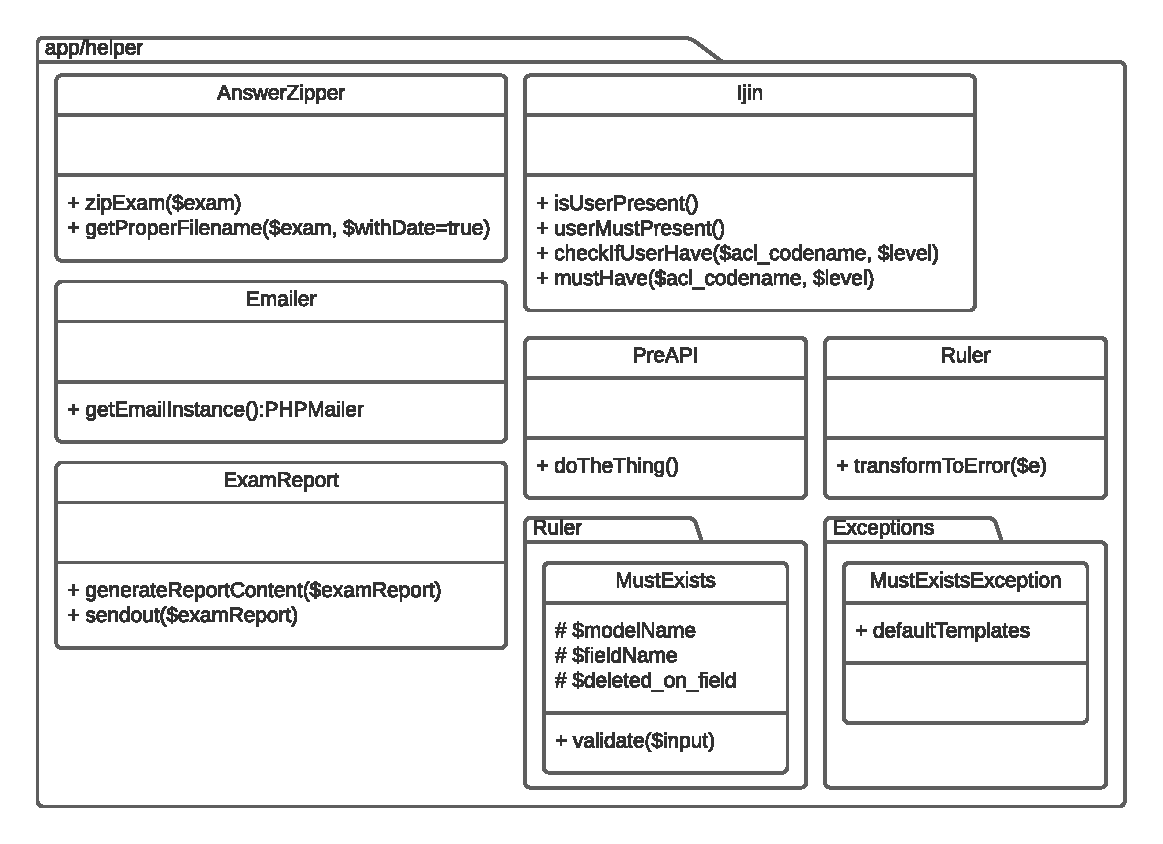
\includegraphics[width=0.75\paperwidth]{Gambar/classmap-be/Classmap - app-helper.pdf}
        \caption{Diagram kelas untuk \textit{namespace} \texttt{Helper}.}
        \label{fig:classmap_app-helper}
    \end{figure}
    Kelas-kelas yang terdapat pada \textit{namespace} ini akan menampung
    berbagai fungsi pembantu yang dapat digunakan tanpa harus diinstansiasi atau
    kelas tambahan untuk perkakas validasi. Diagram kelas untuk
    \textit{namespace} ini dapat diperhatikan pada Gambar
    \ref{fig:classmap_app-helper}.
    
    Kelas-kelas yang terdapat pada \textit{namespace} ini tediri dari
    \begin{itemize}
        \item \texttt{AnswerZipper} Kelas ini bertanggung jawab untuk membuat
            \textit{archive} zip dari ujian tertentu.\\
            Fungsi pada kelas ini terdiri dari:
            \begin{itemize}
                \item \texttt{zipExam(\$exam)} \\
                    Buat \textit{archive} untuk ujian tertentu. \\
                    \textbf{Input:} Objek dari \texttt{Exam}.\\
                    \textbf{Output:} nama berkas zip.
                    
                \item \texttt{getProperFilename(\$exam, \$withDate=true)} \\
                    Bangkitkan nama berkas yang tepat untuk ujian tertentu.\\
                    \textbf{Input:} objek \texttt{exam}, opsi untuk menambahkan
                    tanggal.\\
                    \textbf{Output:} \textit{string} nama berkas.
            \end{itemize}
        
        \item \texttt{Emailer} Kelas ini digunakan untuk membuat dan
            mengkonfigurasi objek \textit{PHPMailer}. Fungsi pada kelas ini
            terdiri dari:
            \begin{itemize}
                \item \texttt{getEmailInstance()} \\
                    Buat objek \texttt{PHPMailer} dan knfigurasi objek tersebut
                    berdasarkan konfigurasi sistem.\\
                    \textbf{Input:} -\\
                    \textbf{Output:} Objek dari \texttt{PHPMailer}.
            \end{itemize}
            
        \item \texttt{Ijin} Kelas ini membantu pengecekan perizinan dengan
            entitas ACL dan ACLItem.
            \begin{itemize}
                \item \texttt{isUserPresent()} \\
                    Melakukan pengecekan apakah kode otentikasi tersedia dan
                    valid. \\
                    \textbf{Input:} -\\
                    \textbf{Output:} \textit{boolean} kehadiran otentikasi yang
                    valid.
                    
                \item \texttt{userMustPresent()} \\
                    Memastikan bahwa token otentikasi ada. \\
                    \textbf{Input:} -\\
                    \textbf{Output:} -, namun dapat melempar eksepsi jika token
                    tidak tersedia.
                    
                \item \texttt{checkIfUserHave(\$acl\_codename, \$level)} \\
                    Melakukan pengecekan apakah token otentikasi memiliki izin
                    untuk melakukan suatu aksi pada \textit{codename}
                    tertentu.\\
                    \textbf{Input:} nama kode izin, perizinan yang seharusnya
                    dimiliki\\
                    \textbf{Output:} \textit{boolean} apakah token memiliki
                    permisi tersebut.
                    
                \item \texttt{mustHave(\$acl\_codename, \$level)} \\
                    Memastikan bahwa token memiliki izin untuk melakukan sesuatu
                    \\
                    \textbf{Input:} nama kode izin, perizinan yang seharusnya
                    dimiliki\\
                    \textbf{Output:} -, namun dapat melempar eksepsi jika token
                    tidak memiliki izin.
            \end{itemize}
            
        \item \texttt{PreAPI} \textit{Macro} untuk API.
            \begin{itemize}
                \item \texttt{doTheThing()} \\
                    Melakukan transformasi badan permintaan API menjadi JSON.
                    Dilakukan hanya pada \textit{HTTP method} \texttt{POST} dan
                    \texttt{PUT}.\\
                    \textbf{Input:} -\\
                    \textbf{Output:} -
            \end{itemize}
        
        \item \texttt{Ruler} \textit{Macro} untuk \textit{library} validasi
            menjadi eksepsi kelas \texttt{Model/Error}.
            \begin{itemize}
                \item \texttt{transformToError(\$e)} \\
                    Melakukan transformasi eksepsi dari \textit{library}
                    validasi, menjadi \texttt{Model/Error} \\
                    \textbf{Input:} -\\
                    \textbf{Output:} -
            \end{itemize}
            
        \item \texttt{Ruler\textbackslash MustExists} Kelas peraturan untuk
            validasi tambahan. Memastikan apakah suatu entri terdapat pada
            sebuah tabel. Kelas ini memiliki atribut sebagai berikut:
            \begin{itemize}
                \item \texttt{\$modelName}: Nama model
                \item \texttt{\$fieldName}: Nama kolom kunci primer dari model
                \item \texttt{\$deleted\_on\_field}: Nama kolom \textit{soft
                delete} dari model
            \end{itemize}
            Serta fungsi sebagai berikut:
            \begin{itemize}
                \item \texttt{validate(\$input)} \\
                    Melakukan validasi bahwa data yang diberikan terdapat pada
                    tabel.\\
                    \textbf{Input:} input data\\
                    \textbf{Output:} \textit{boolean} kebenaran dari validasi
                    tersebut.
            \end{itemize}
            
        \item \texttt{Exceptions\textbackslash MustExistsException} Eksepsi oleh
            aturan \textit{MustExists}.
            \begin{itemize}
                \item \texttt{\$defaultTemplates}: Pesan kesalahan pada saat
                validasi gagal.
            \end{itemize}
            Serta fungsi sebagai berikut:
            \begin{itemize}
                \item \texttt{validate(\$input)} \\
                    Melakukan validasi bahwa data yang diberikan terdapat pada
                    tabel.\\
                    \textbf{Input:} input data\\
                    \textbf{Output:} \textit{boolean} kebenaran dari validasi
                    tersebut.
            \end{itemize}
    \end{itemize}

\subsubsection{\textit{Namespace} \texttt{Output}}
    \begin{figure}
        \centering
        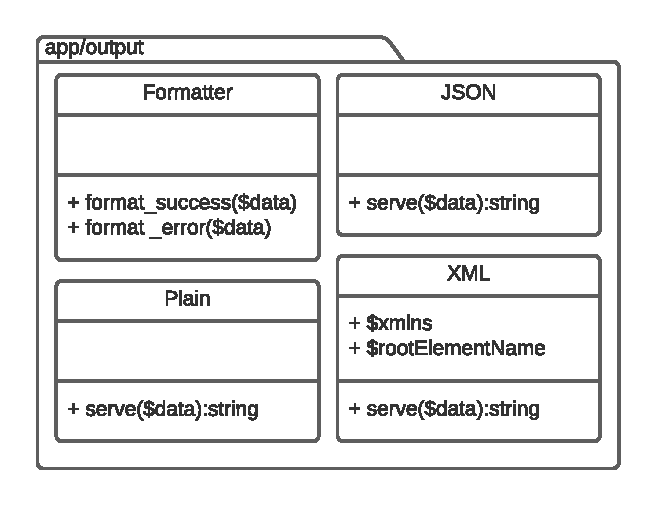
\includegraphics{Gambar/classmap-be/Classmap - app-output.pdf}
        \caption{Diagram kelas untuk \textit{namespace} \texttt{Output}.}
        \label{fig:classmap_app-output}
    \end{figure}
    \textit{Namespace} \texttt{output} menyimpan kelas yang membantu untuk
    formatisasi API. Format yang didukung saat ini berbentuk JSON, XML, dan teks
    biasa. Rancangan diagram kelas ini dapat dilihat pada Gambar
    \ref{fig:classmap_app-output}.
    
    Kelas-kelas yang terdapat pada \textit{namespace} ini terdiri dari
    \begin{itemize}
        \item \texttt{Formatter} \\
            Kelas ini bertanggung jawab untuk melakukan formating utama untuk
            jenis respon sukses dan gagal. Kelas ini memiliki fungsi:
            \begin{itemize}
                \item \texttt{format\_success(\$data)} \\
                    Melakukan format untuk jenis respon sukses.\\
                    \textbf{Input:} input data\\
                    \textbf{Output:} \textit{array}.
                    
                \item \texttt{format\_error(\$data)} \\
                    Melakukan format untuk jenis respon gagal.\\
                    \textbf{Input:} objek dari \texttt{model/Error}\\
                    \textbf{Output:} \textit{array}.
            \end{itemize}
            
        \item \texttt{JSON} \\
            Kelas ini bertanggung jawab untuk melakukan performatan data ke
            bentuk JSON. Kelas ini memiliki fungsi:
            \begin{itemize}
                \item \texttt{serve(\$data)} \\
                    Merepresentasikan data dalam bentuk JSON.\\
                    \textbf{Input:} input data\\
                    \textbf{Output:} \textit{string}.
            \end{itemize}
            
        \item \texttt{Plain} \\
            Kelas ini bertanggung jawab untuk melakukan performatan data ke
            bentuk teks biasa. Kelas ini memiliki fungsi:
            \begin{itemize}
                \item \texttt{serve(\$data)} \\
                    Merepresentasikan data dalam bentuk teks.\\
                    \textbf{Input:} input data\\
                    \textbf{Output:} \textit{string}.
            \end{itemize}
            
        \item \texttt{XML} \\
            Kelas ini bertanggung jawab untuk melakukan performatan data ke
            bentuk JSON. Kelas ini memiliki atribut:
            \begin{itemize}
                \item \texttt{\$xmlns}: \textit{Namespace} yang digunakan untuk
                mendefinisikan XML.
                \item \texttt{\$rootElementName}: Nama elemen pangkal yang akan
                digunakan.
            \end{itemize}
            Kelas ini memiliki fungsi:
            \begin{itemize}
                \item \texttt{serve(\$data)} \\
                    Merepresentasikan data dalam bentuk XML.\\
                    \textbf{Input:} input data\\
                    \textbf{Output:} \textit{string}.
            \end{itemize}
    \end{itemize}
    
\subsection{\textit{Namespace} \texttt{Service}, \texttt{Cronjob} dan
\texttt{View}}
    \begin{figure}
        \centering
        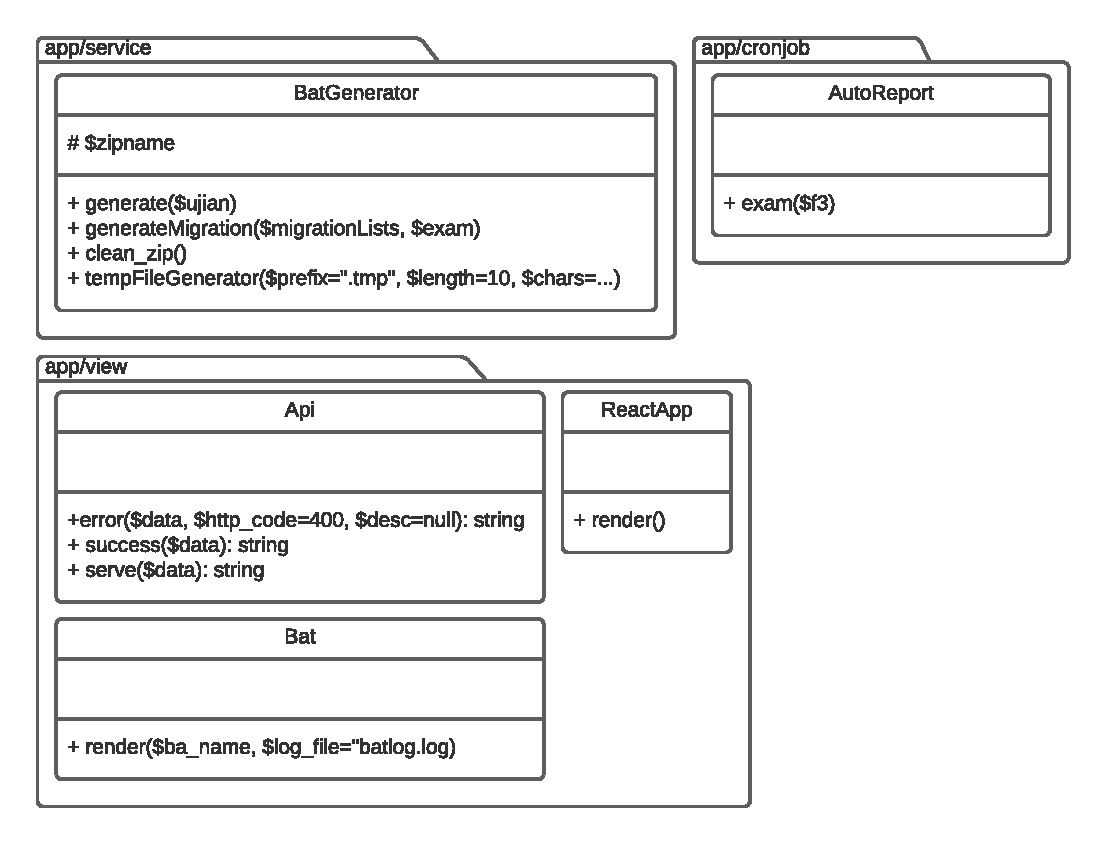
\includegraphics[width=0.75\paperwidth]{Gambar/classmap-be/Classmap - app-service,cronjob,view.pdf}
        \caption{Diagram kelas untuk \textit{namespace} \texttt{Service},
            \texttt{Cronjob} dan \texttt{View}.}
        \label{fig:classmap_app-service,cronjob,view}
    \end{figure}
    Diagram kelas untuk beberapa \textit{Namespace} ini dapat dilihat pada
    Gambar \ref{fig:classmap_app-service,cronjob,view}. Kelas-kelas pada
    \textit{namespace} ini terdiri dari:
    \begin{itemize}
        \item \texttt{Service\textbackslash Batgenerator} \\
            Kelas ini bertanggung jawab untuk membuat \textit{script} bat untuk
            ujian dan migrasi. Atribut yang terdapat pada kelas ini:
            \begin{itemize}
                \item \texttt{\$zipname}: Nama berkas zip sebelumnya
            \end{itemize}
            Fungsi yang terdapat pada kelas ini:
            \begin{itemize}
                \item \texttt{generate(\$ujian)} \\
                    Bertanggung jawab untuk melakukan pembuatan \textit{script}
                    bat untuk ujian. \\
                    \textbf{Input:} Objek \texttt{Exam}.\\
                    \textbf{Output:} \textit{string} nama berkas zip.
                
                \item \texttt{generateMigration(\$migrationLists, \$exam)} \\
                    Bertanggung jawab untuk melakukan pembuatan \textit{script}
                    bat untuk perpindahan peserta.\\
                    \textbf{Input:} Daftar migrasi, dan objek \texttt{Exam}\\
                    \textbf{Output:} \textit{string} nama berkas zip.
                
                \item \texttt{clean\_zip()} \\
                    Menghapus berkas zip \\
                    \textbf{Input:} -\\
                    \textbf{Output:} -
                
                \item \texttt{tempFileGenerator(\$prefix=".tmp", \$length=10,
                \$chars=...)} \\
                    Membangkitkan nama sementara untuk zip. \\
                    \textbf{Input:} prefixks untuk nama berkas sementara,
                        panjang teks acak, dan daftar karakter yang ingin
                        digunakan.\\
                    \textbf{Output:} \textit{string} nama berkas sementara.
            \end{itemize}
        
        \item \texttt{Cronjob\textbackslash Autoreport} \\
            Kelas ini bertanggung jawab untuk melakukan tugas \textit{cron}
            untuk mengirimkan laporan. Fungsi yang terdapat pada kelas ini
            adalah:
            \begin{itemize}
                \item \texttt{exam(\$f3)} \\
                    Bertanggun jawab untuk mengkompilasi ujian yang telah
                    selesai, dan mengirimkan email ke daftar yang disebutkan
                    pada entri. \textbf{Input:} Instansi kelas \texttt{Base}
                    dari framework.\\
                    \textbf{Output:} -
            \end{itemize}
            
        \item \texttt{View\textbackslash Api} \\
            Kelas ini didedikasikan untuk menyediakan API dengan format tertentu
            yang didukung oleh kelas yang terdapat pada namespace
            \texttt{Output}. Fungsi yang terdapat pada kelas ini adalah:
            \begin{itemize}
                \item \texttt{error(\$data, \$http\_code=400, \$desc=null)} \\
                    Bertanggung jawab untuk melakukan peformatan \textit{error}.
                    \\
                    \textbf{Input:} objek \texttt{Error}, kode respon HTTP, dan
                    deskripsinya.\\
                    \textbf{Output:} \textit{string}.
                    
                \item \texttt{success(\$data)} \\
                    Bertanggung jawab untuk melakukan peformatan data untuk
                    respon sukses. \\
                    \textbf{Input:} \textit{array} data.\\
                    \textbf{Output:} \textit{string}.
                
                \item \texttt{serve(\$data)} \\
                    Menyajikan data ke pengkonsumsi API, sesuai dengan format
                    yang diminta oleh pengkonsumsi API, seperti JSON, XML,
                    ataupun teks biasa.\\
                    \textbf{Input:} \textit{string} data.\\
                    \textbf{Output:} \textit{string}.
            \end{itemize}
            
        \item \texttt{View\textbackslash Bat} \\
            Melakukan pembuatan \textit{script} bat berdasarkan
            \textit{template} yang telah diberikan, dengan memanfaatkan
            \textit{templating engine} yang disediakan oleh \textit{framework}.
            Fungsi yang terdapat pada kelas ini adalah:
            \begin{itemize}
                \item \texttt{render(\$ba\_name, \$log\_file="batlog.log")} \\
                    \textit{Render template} yang diberikan, dan kembalikan
                    sebagai \textit{string}. \\
                    \textbf{Input:} Nama \textit{template}, nama log yang akan
                    digenerasi.\\
                    \textbf{Output:} \textit{string}.
            \end{itemize}
        
        \item \texttt{View\textbackslash Reactapp} \\
            Bertanggung jawab untuk menyajikan aplikasi React untuk tampilan
            publik.
            \begin{itemize}
                \item \texttt{render()} \\
                    Sajikan hasil \textit{build} dari React. \\
                    \textbf{Input:} -\\
                    \textbf{Output:} -
            \end{itemize}
    \end{itemize}


\section{Perancangan Sistem CI/CD dan Unit Testing}
    % melakukan build pada saat commit
    Berdasarkan hasil analisis pada bab sebelumnya, penelitian membutuhkan
    sebuah sistem yang dapat melakukan \textit{build} secara otomatis sebelum
    dapat di-\textit{deploy} ke server produksi. Sistem \textit{build} tersebut
    akan direncanakan untuk diimplementasi pada sistem CI/CD yang terintegrasi
    dengan tempat penyimpanan repositori kode sumber. Kode sumber tersebut
    nantinya akan di\textit{track} oleh sistem repositori sehingga pada saat
    kode mengalami perubahan, sistem CI/CD akan secara otomatis berjalan. Sistem
    ini dirancang untuk melakukan hal berikut secara sekuensial:
    
    \begin{itemize}
        \item Melakukan penyegaran dependensi.
        \item Melakukan \textit{build} dengan level produksi.
        \item Menyimpan hasil \textit{build} pada repositori.
        \item Unggah perubahan pada repositori kembali ke layanan penyimpanan.
        \item Picu sistem \textit{deploy} untuk melakukan \textit{deployment}.
    \end{itemize}
    
    Hal tersebut dilakukan untuk memastikan hasil \textit{build} dapat
    dikirimkan pada server untuk disediakan ke pengguna. Sistem
    \textit{deployment} yang digunakan diimplementasi dengan bantuan script yang
    dijalankan via SSH. \textit{Script} tersebut dirancang akan melakukan
    pengunduhan perubahan kode, lalu melakukan penyegaran dependensi versi
    server, dan mengabari kembali sistem CI/CD bahwa \textit{deployment} telah
    berhasil dilakukan.
    
    % Unit testing part
    Selain melakukan \textit{build}, penelitian juga akan menambahkan sistem tes
    unit otomatis. Sistem tes ini direncakan untuk melakukan pengecekan terhadap
    komponen-komponen krusial pada aplikasi. Karena konsekuensi yang ditanggung
    aplikasi cukup besar, maka sistem tes ditambahkan untuk mencegah kesalahan
    yang sangat fatal. Sistem tes unit ini direncakan berjalan bersama sistem
    \textit{build}. Sehingga kode akan di tes setiap kali kode baru diunggah ke
    tempat penyimpanan.